\documentclass[11pt,          % font size: 11pt or 12pt
               phd,           % degree:    ms or phd
               doublespacing % spacing: onehalfspacing or doublespacing
               ]{ncsuthesis}

%%----------------------------------------------------------------------------%%
%%------------------------------ Bugs ----------------------------------------%%

% Dont put \center\caption, cause missing \item error
% use \caption only

%%----------------------------------------------------------------------------%%

%%----------------------------------------------------------------------------%%
%%------------------------------ Import Packages -----------------------------%%
%%----------------------------------------------------------------------------%%

\usepackage{booktabs}  % professionally typeset tables
\usepackage{amsmath}%,amssymb,amsfonts}
\usepackage{textcomp}  % better copyright sign, among other things
%\usepackage{xcolor}
\usepackage{lipsum}    % filler text
% LEE \usepackage{subfig}    % composite figures
\usepackage{outlines} % for bullets
\usepackage{enumitem}
\usepackage{adjustbox}

\usepackage[%
    font={small,sf},
    labelfont=bf,
    format=hang,    
    format=plain,
    margin=0pt,
    width=0.8\textwidth,
]{caption}
%\usepackage{subfig}
\usepackage[list=true]{subcaption}

\usepackage{url}

\usepackage{enumitem}

\usepackage{geometry} 
\usepackage{units}
\usepackage[binary-units=true]{siunitx}
\usepackage{pst-plot}
\usepackage{pgfplots}
\usepackage{rotating}
\usepackage{adjustbox}
\usepackage{multirow}

\usepackage{acro}

% for quotes
\usepackage[utf8]{inputenc}
\usepackage{quotchap}
\usepackage{epigraph}
\usepackage{quotchap}
\usepackage{csquotes}

% Highlighting
\usepackage{color,soul}
\newcommand{\hlc}[2][yellow]{{%
    \colorlet{foo}{#1}%
    \sethlcolor{foo}\hl{#2}}%
}


% help reduce whitespace
%\usepackage{savetrees}
%%ORTIZ PACKAGES


%%%%%%%%%%%%%%%%%%%%%%%%%%%%%%%%%%%%%%%%%%
%%%%%%%%%%% Old bibliography commands
%%%%%%%%%%%%%%%%%%%%%%%%%%%%%%%%%%%%%%%%%%5
%\usepackage[super,sort&compress,comma,square,authoryear]{natbib} %\cite command %Added by Ortiz

%use the following line with plainnat
%\usepackage[super,sort&compress,comma,square,numbers]{natbib} %\cite command %Added by Ortiz
%\usepackage{natbib}

%\usepackage[style=alphabetic,natbib=true,backend=bibtex
%sorting=nyt,firstinits=true,isbn=false,doi=false,url=false]{biblatex} %couldn't get backend=biber to work

%\usepackage{filecontents}

%\bibliography{Ortiz-thesis2}
%\bibliographystyle{plain}


%%%%%%%%%%%%%%%%%%%%%%%%%%%%%%%%%%%%%%%%%%
%%%%%%%%%%% Hack for alphanumeric bibliography
%%%%%%%%%%%%%%%%%%%%%%%%%%%%%%%%%%%%%%%%%%5
\RequirePackage[
			style=alphabetic,%numeric-comp,%authoryear-comp,%
			sorting=nyt,%ynt					
			hyperref=true, %	
			firstinits=true,%
			backend=bibtex,
			natbib=true,
			url=false,
			isbn=false,
			maxnames=2, %for et al to be used
			maxalphanames=1, %to avoid printing a + for every et al in the abbreviation
			doi=false]{biblatex}		
			

%needed to do et al after two names
%http://tex.stackexchange.com/questions/44048/use-et-al-in-biblatex-custom-style
\renewcommand*{\finalnamedelim}{\addspace\&\space}

%Simplify abbreviation (the default uses either one or two authors and it indicates et al with a +)
%The following five lines make it so that only the first author is used in the abbreviation
%http://tex.stackexchange.com/questions/27956/label-only-from-first-author
\renewcommand*{\labelalphaothers}{}
    \renewcommand*{\intitlepunct}{}
    \DefineBibliographyStrings{german}{in={}}
    \DefineBibliographyStrings{english}{in={}}
    \DeclareNameAlias{sortname}{last-first}
    \DeclareNameAlias{default}{last-first}
	
%\AtEveryCitekey{\ifciteseen{}{\defcounter{maxnames}{99}}} %authoryear			
\DeclareFieldFormat[article,periodical]{volume}{\mkbibbold{#1}}
\makeatletter

\newrobustcmd*{\parentexttrack}[1]{%
  \begingroup
  \blx@blxinit
  \blx@setsfcodes
  \blx@bibopenparen#1\blx@bibcloseparen
  \endgroup}

\AtEveryCite{%
  \let\parentext=\parentexttrack%
  \let\bibopenparen=\bibopenbracket%
  \let\bibcloseparen=\bibclosebracket}

\makeatother
\renewcommand{\cite}[1]{\parencite{#1}}


\renewbibmacro{in:}{%
  \ifentrytype{article}{}{%
  \printtext{\bibstring{in}\intitlepunct}}}
  
\AtEveryBibitem{\clearfield{month}}

\AtEveryBibitem{\clearfield{language}}
%%%%%%%%%%%%%%%%%%%%%%%%%%%%%%%%%%%%%%%%%%%%%

%\addbibresource{Ortiz-thesis2.bib}
%\addbibresource{Ortiz-thesisURL.bib}
\addbibresource{LeeBaker-thesis.bib}

 \defbibheading{myheading}[BIBLIOGRAPHY]{
 \chapter*{#1}
 %\centerline{\bf{#1}}
 \markboth{#1}{#1}}

%\usepackage{amsmath,amssymb,amsfonts} %amssymb and amsfonts cannot be used in conjunction with mdput
%\usepackage{graphicx,subfig}% Include figure files
\usepackage{dcolumn}% Align table columns on decimal point
\usepackage{bm}% bold math
%\usepackage{hyperref}% add hypertext capabilities
%\usepackage{hypernat}% make hyperref and natbib work together
\usepackage{cancel}
\usepackage{verbatim}% multiline commenting
\usepackage{ifthen}
\usepackage{url}
\usepackage{sectsty}
\usepackage{balance} 
%\usepackage{caption}
\usepackage{graphicx} %eps figures can be used instead
\usepackage{lastpage}
\usepackage[format=plain,justification=RaggedRight,singlelinecheck=false,font=small,labelfont=bf,labelsep=space]{caption} 
\usepackage{fancyhdr}
\pagestyle{fancy}

%http://tex.stackexchange.com/questions/100817/error-when-using-bc-from-abbrevs-in-caption
%Getting BC
\usepackage{abbrevs}
\usepackage{etoolbox}
\robustify{\DateMark} % after having loaded abbrevs

\usepackage{units} %Needed to solve bug from citation Hydrodynamics in 21/2 dimensions
%see http://www.latex-community.org/viewtopic.php?f=5&t=989

\usepackage[sharp]{easylist} %used for brainstorming purposes 
%\usepackage{mathabx} % used for \Asterisk for convolution %conflicts with \widering

%compile on single pass
%\usepackage[backend=biber,...]{biblatex}


%%%%%%%%%%%%
%%% Hack to make chapters start on odd pages
% http://tex.stackexchange.com/questions/73591/how-to-have-a-blank-even-page-before-every-chapter
%%%%%%%%%%%%
%\newcommand{\ensureoddstart}{\checkoddpage\ifoddpage\else\newpage\mbox{}\fi}
%\newcommand{\ensureoddstart}{}


%%%Fancy tables
%http://tex.stackexchange.com/questions/94032/fancy-tables-in-latex
% Lee \usepackage[table]{xcolor}
% Lee \usepackage{array,booktabs}
% Lee \usepackage{colortbl}
% Lee \newcolumntype{L}{@{}>{\kern\tabcolsep}l<{\kern\tabcolsep}}



%%%%%%%%%%
%%%%% Hack to allow more levels in outline
%%%%%%%%%%
%\setcounter{secnumdepth}{5}
\setcounter{tocdepth}{5} %may violate ETD
%Usage http://pleasemakeanote.blogspot.com/2010/06/how-to-activate-subsubsubsection-in.html
%\section{} % level 1
%\subsection{} % level 2
%\subsubsection{} % level 3
%\paragraph{} % level 4 - equivalent to subsubsubsection
%\subparagraph{} % level 5

%http://tex.stackexchange.com/questions/60209/how-to-add-an-extra-level-of-sections-with-headings-below-subsubsection
\usepackage{titlesec}

\setcounter{secnumdepth}{4}

\titleformat{\paragraph}
{\normalfont\normalsize\bfseries}{\theparagraph}{1em}{}
\titlespacing*{\paragraph}
{0pt}{3.25ex plus 1ex minus .2ex}{1.5ex plus .2ex}

%%%%%%%%%%%%%%%%%%%%%%%%%%
%%%% Hack for containing figures within sections
%%%%%%%%%%%%%%%%%%%%%%%%%%%%
%http://ctan.org/pkg/placeins
\usepackage{placeins}
%De�fines a \FloatBar�rier com�mand, be�yond which floats may not pass; use�ful, for ex�am�ple, to en�sure all floats for a sec�tion ap�pear be�fore the next \sec�tion com�mand.

%%%Hack for centering all figures
%\makeatletter
%\g@addto@macro\@floatboxreset\centering
%\makeatother

%%----------------------------------------------------------------------------%%
%%---------------------------- Formatting Options ----------------------------%%
%%----------------------------------------------------------------------------%%
%%

%% -------------------------------------------------------------------------- %%
%% Disposition format -- any titles, headings, section titles
%%  These formatting commands affect all headings, titles, headings,
%%  so sizing commands should not be used here.
%%  Formatting options to consider are
%%     +  \sffamily - sans serif fonts.  Dispositions are often typeset in
%%                    sans serif, so this is a good option. 
%%     +  \rmfamily - serif fonts
%%     +  \bfseries - bold face
%\dispositionformat{\sffamily\bfseries}   % bold and sans serif
\dispositionformat{\bfseries}            % bold and serif

%% -------------------------------------------------------------------------- %%
%% Formatting for centered headings - Abstract, Dedication, etc. headings
%%  This is where one might put a sizing command.
%%  \MakeUppercase can be used to typeset all headings in uppercase.
\headingformat{\large\MakeUppercase}   % All letters uppercase
%\headingformat{\large}                % Not all uppercase
%\headingformat{\Large\scshape}        % Small Caps, used with serif fonts.

%% Typographers recommend using a normal inter-word space after
%% sentences. TeX's default is to add an wider space, but \frenchspacing
%% gives a normal spacing. Comment out the following line if you prefer
%% wider spaces between sentences.
\frenchspacing


%% -------------------------------------------------------------------------- %%
%%  Optional packages
%%    A number of compatible packages to improve the look and feel of
%%    your document are available in the file optional.tex 
%%    (For example, hyperlinks, fancy chapter headings, and fonts)
%% To use these options, uncomment the next line and see optional.tex
%%  Optional Packages to consider.   These packages are compatible with
%%    ncsuthesis.  

%% -------------------------------------------------------------------------- %%
%% Fancy chapter headings
%%  available options: Sonny, Lenny, Glenn, Conny, Rejne, Bjarne
%\usepackage[Sonny]{fncychap}
\usepackage[Rejne]{fncychap}

%%----------------------------------------------------------------------------%%
%% Hyperref package creates PDF metadata and hyperlinks in Table of Contents
%%  and citations.  Based on feedback from the NCSU thesis editor, 
%%  the links are not visually distinct from normal text (i.e. no change
%%  in color or extra boxes).
\usepackage[
  pdfauthor={Carlos Pompeyo Ortiz},
  pdftitle={Rigidity of Microsphere Heaps},
  pdfcreator={pdftex},
  pdfsubject={NC State ETD Thesis},
  pdfkeywords={microfluidics, hard sphere, jamming, suspension, rigidity, friction, microscopy},
  colorlinks=true,
  linkcolor=black,
  citecolor=black,
  filecolor=black,
  urlcolor=black,
]{hyperref}


%% -------------------------------------------------------------------------- %%
%% Microtype - If you use pdfTeX to compile your thesis, you can use
%%              the microtype package to access advanced typographic
%%              features.  By default, using the microtype package enables
%%              character protrusion (placing glyphs a hair past the right 
%%              margin to make a visually straighter edge)
%%              and font expansion (adjusting font width slightly to get 
%%              more favorable justification).
%%              Using microtype should decrease the number of lines
%%              ending in hyphens.
\usepackage{microtype}


%%----------------------------------------------------------------------------%%
%% Fonts 

%% ETD guidelines don't specify the font.  You can enable the fonts
%%  by uncommenting the appropriate lines.  Using the default Computer 
%%  Modern fonts is *not* required.  A few common choices are below.
%%  See http://www.tug.dk/FontCatalogue/ for more options.

%% Serif Fonts -------------------------------------------------
%%  The four serif fonts listed here (Utopia, Palatino, Kerkis,
%%  and Times) all have math support.


%% Utopia
\usepackage[T1]{fontenc}
\usepackage[adobe-utopia]{mathdesign}

%% Palatino
%\usepackage[T1]{fontenc}
%\usepackage[sc]{mathpazo}
%\linespread{1.05}

%% Kerkis
%\usepackage[T1]{fontenc}
%\usepackage{kmath,kerkis}

%% Times
%\usepackage[T1]{fontenc}
%\usepackage{mathptmx}


%% Sans serif fonts -------------------------

%\usepackage[scaled]{helvet}  % Helvetica
%\usepackage[scaled]{berasans} % Bera Sans

%solve bug from fancyhdr in optional
%http://nw360.blogspot.com/2006/11/latex-headheight-is-too-small.html
\setlength{\headheight}{14pt}

%%----------------------------------------------------------------------------%%
%%---------------------------- Content Options -------------------------------%%
%%----------------------------------------------------------------------------%%
%% Size of committee: 3, 4, 5, or 6 -- this number includes the chair
\committeesize{4}

%% Members of committee
%%  Each of the following member commands takes an optional argument
%%   to specify their role on the committee.
%%  For co-chairs, use the commands:
%%      \cochairI{Doug Dodd}
%%      \cochairII{Chris Cox}
%%
\chair{Paul Franzon}
\memberI{Winser Alexander}
\memberII{Gregory Byrd}
\memberIII{Richard Warr}   % unnecessary if committeesize=3


%% Student writing thesis, \student{First Middle}{Last}
\student{Lee B.}{Baker} % a full middle name
%\student{John Mark}{Smith} % a full middle name
%\student{John M.}{Smith} % a middle initial

%% Degree program
\program{Electrical Engineering}

%% Thesis Title
%%  Keep in mind, according to ETD guidelines:
%%    +  Capitalize first letter of important words.
%%    +  Use inverted pyramid shape if title spans more than one line.
%%
%%  Note: To break the title onto multiple lines, use \break instead of \\.
%\thesistitle{A North Carolina State University Sample \LaTeX{} Thesis \break 
%with a Title So Long it Needs a Line Break}
\thesistitle{Design of a 3DIC system to aid in the acceleration of edge systems that \break employ multiple instances of disparate artificial neural networks}

%% Degree year.  Necessary if your degree year doesn't equal the current year.
%\degreeyear{1995}


%%----------------------------------------------------------------------------%%
%%---------------------------- Personal Macros -------------------------------%%
%%----------------------------------------------------------------------------%%

%% A central location to add your favorite macros.

%% A few examples to get you started.
\newcommand{\uv}[1]{\ensuremath{\mathbf{\hat{#1}}}}
\newcommand{\bo}{\ensuremath{\mathbf{\Omega}}}
\newcommand{\eref}[1]{Eq.~\ref{#1}}
\newcommand{\fref}[1]{Fig.~\ref{#1}}
\newcommand{\tref}[1]{Table~\ref{#1}}
\newcommand{\del}{\nabla}
\renewcommand{\exp}[1]{e^{#1}}
\newcommand{\Conv}{\mathop{\scalebox{1.5}{\raisebox{-0.2ex}{$\ast$}}}}%


\usepackage{color}
%\newcommand{\NEW}[1]{\textcolor{blue}{#1}}
\newcommand{\NEW}[1]{#1}
\newcommand{\COMMENT}[1]{\textcolor{green}{#1}}


\newcommand{\NOTER}[1]{\textcolor{orange}{#1}}
\newcommand{\NOTEC}[1]{\textcolor{blue}{#1}}
\newcommand{\NOTEK}[1]{\textcolor{magenta}{#1}}

\newcommand{\mum}{\ensuremath{{\mu}\text{m}}}

%This makes it so that you can add short paths in your .tex by including the folders where you store your images in the search path
\graphicspath{{./Introduction/figs/}{./ANNs/figs/}{./3DIC/figs/}{./DRAM/figs/}{./SystemOverview/figs/}{./Results/figs/}{./ConclusionsAndFutureWork/figs/}{./Motivation/figs/}{./SystemOperations/figs/}{./DetailedSystemDescription/figs/}{./StateOfTheArt/figs/}{../../../../3DSystem/DOC/wikiImages/}{./wikiImages/}{./eps/}}


%%----------------------------------------------------------------------------%%
%%---------------------------- Plotting --------------------------------------%%
%%----------------------------------------------------------------------------%%
%% Added Lee

% axis style
\pgfplotsset{every axis/.append style={
                    axis x line=middle,    % put the x axis in the middle
                    axis y line=middle,    % put the y axis in the middle
                    axis line style={<->}, % arrows on the axis
                    xlabel={$x$},          % default put x on x-axis
                    ylabel={$y$},          % default put y on y-axis
                    }}
% grid style
\pgfplotsset{
  grid style = {
    dash pattern = on 0.05mm off 1mm,
    line cap = round,
    black,
    line width = 0.5pt
  }
}
% line style
\pgfplotsset{myBlueStyle/.style={color=blue,no marks,line width=1pt,-}} 
\pgfplotsset{myBlackStyle/.style={color=blue,no marks,line width=1pt,-}} 
\pgfplotsset{myBlueThickStyle/.style={color=blue,no marks,line width=2pt,-}} 
\pgfplotsset{myBlackThickStyle/.style={color=black,no marks,line width=2pt,-}} 

% arrow style: stealth stands for 'stealth fighter' 
\tikzset{>=stealth}

%\DeclarePairedDelimiter\ceil{\lceil}{\rceil}
%\DeclarePairedDelimiter\floor{\lfloor}{\rfloor}

%%---------------------------------------------------------------------------%%
\usepackage{calc}
%% Capital letter height
\newlength{\chaptercapitalheight}
\settoheight{\chaptercapitalheight}{D}
\newlength{\chapterfootskip}
\setlength{\chapterfootskip}{\chaptercapitalheight}
\addtolength{\chapterfootskip}{2\baselineskip}
\addtolength{\chapterfootskip}{0.5ex}  % A little extra space to ensure there are 2 full double spaced lines
%\def\chapterfootskipnum{\chapterfootskip}
\renewcommand{\listfigurename}{LIST OF FIGURES}
\renewcommand{\listtablename}{LIST OF TABLES}
\renewcommand{\bibname}{BIBLIOGRAPHY}

%\renewcommand{\cfttoctitlefont}{\centering\ncsu@headingformat}


%http://tex.stackexchange.com/questions/47184/height-of-figure-caption-textheight
\newlength\graphht
\newcommand\calculategraphicstargetheight[1]{%
     \setlength\graphht{\textheight 
                       -\parskip
                       -\abovecaptionskip -\belowcaptionskip
                       -(12pt * #1) % assuming baselineskip of 12pt in caption
                       -\chapterfootskip
                       }}

%\usepackage{titlesec}

%landscape support in fancyhdr from http://tex.stackexchange.com/questions/9071/how-to-translate-and-rotate-the-heading-of-landscaped-pages
\usepackage{pdflscape}
\usepackage{tikz}
\fancypagestyle{lscapedplain}{%
  \fancyhf{}
  \fancyfoot{%
    \tikz[remember picture,overlay]
      \node[outer sep=1cm,above,rotate=90] at (current page.east) {\thepage};}
\renewcommand{\headrulewidth}{0pt} 
\renewcommand{\footrulewidth}{0pt}
}

\DeclareAcronym{nn}{
  short = NN ,
  long  = Neural Network ,
  short-plural = s ,
  long-plural  = s ,
  class = abbrev
}

\DeclareAcronym{ann}{
  short = ANN ,
  long  = Artificial Neural Network ,
  short-plural = s ,
  long-plural  = s ,
  class = abbrev
}

\DeclareAcronym{an}{
  short = ANe ,
  long  = Artificial Neuron ,
  short-plural = s ,
  long-plural  = s ,
  class = abbrev
}

\DeclareAcronym{cnn}{
  short = CNN ,
  long  = Convolutional Neural Network ,
  short-plural = s ,
  long-plural  = s ,
  class = abbrev
}

\DeclareAcronym{dnn}{
  short = DNN ,
  long  = Deep Neural Network ,
  short-plural = s ,
  long-plural  = s ,
  class = abbrev
}

\DeclareAcronym{ic}{
  short = IC ,
  long  = Integrated Circuit ,
  short-plural = s ,
  long-plural  = s ,
  class = abbrev
}

\DeclareAcronym{asic}{
  short = ASIC ,
  long  = Application-Specific Integrated Circuit ,
  short-plural = s ,
  long-plural  = s ,
  class = abbrev
}

\DeclareAcronym{asip}{
  short = ASIP ,
  long  = Application-Specific Instruction-set Processor ,
  short-plural = s ,
  long-plural  = s ,
  class = abbrev
}

\DeclareAcronym{eda}{
  short = EDA ,
  long  = Electronic Design Automation ,
  class = abbrev
}

\DeclareAcronym{fpu}{
  short = FPU ,
  long  = Floating-point Unit ,
  short-plural = s ,
  long-plural  = s ,
  class = abbrev
}

\DeclareAcronym{fp}{
  short = FP ,
  long  = floating-point ,
  class = abbrev
}

\DeclareAcronym{mac}{
  short = MAC ,
  long  = Multiply-Accumulate Unit ,
  short-plural = s ,
  long-plural  = s ,
  class = abbrev
}

\DeclareAcronym{alu}{
  short = ALU ,
  long  = Arithmetic Logic Unit ,
  short-plural = s ,
  long-plural  = s ,
  class = abbrev
}

\DeclareAcronym{msb}{
  short = MSB ,
  long  = Most Significant Bit ,
  short-plural = s ,
  long-plural  = s ,
  class = abbrev
}

\DeclareAcronym{lsb}{
  short = LSB ,
  long  = Least Significant Bit ,
  short-plural = s ,
  long-plural  = s ,
  class = abbrev
}

\DeclareAcronym{soc}{
  short = SoC ,
  long  = System-on-Chip ,
  short-plural = s ,
  long-plural  = s ,
  class = abbrev
}

\DeclareAcronym{noc}{
  short = NoC ,
  long  = Network-on-Chip ,
  short-plural = s ,
  long-plural  = s ,
  class = abbrev
}

\DeclareAcronym{isa}{
  short = ISA ,
  long  = Instruction Set Architecture ,
  short-plural = s ,
  long-plural  = s ,
  class = abbrev
}

\DeclareAcronym{simd}{
  short = SIMD ,
  long  = Single-Instruction Multiple-Data ,
  short-plural = s ,
  long-plural  = s ,
  class = abbrev
}

\DeclareAcronym{stop}{
  short = StOp ,
  long  = Streaming Operation ,
  short-plural = s ,
  long-plural  = s ,
  class = abbrev
}

\DeclareAcronym{vliw}{
  short = VLIW ,
  long  = Very-Long Instruction Word ,
  short-plural = s ,
  long-plural  = s ,
  class = abbrev
}

\DeclareAcronym{sram}{
  short = SRAM ,
  long  = Static Random Access Memory ,
  short-plural = s ,
  long-plural  = s ,
  class = abbrev
}

\DeclareAcronym{dram}{
  short = DRAM ,
  long  = Dynamic Random Access Memory ,
  short-plural = s ,
  long-plural  = s ,
  class = abbrev
}

\DeclareAcronym{3dic}{
  short = 3DIC ,
  long  = Three-Dimensional Integrated Circuit ,
  short-plural = s ,
  long-plural  = s ,
  class = abbrev
}

\DeclareAcronym{3ddram}{
  short = 3D-DRAM ,
  long  = Three-Dimensional Dynamic Random Access Memory ,
  class = abbrev
}

\DeclareAcronym{pe}{
  short = PE ,
  long  = Processing Engine ,
  short-plural = s ,
  long-plural  = s ,
  class = abbrev
}

\DeclareAcronym{pc}{
  short = PC ,
  long  = Program Counter ,
  short-plural = s ,
  long-plural  = s ,
  class = abbrev
}

\DeclareAcronym{tsv}{
  short = TSV ,
  long  = Through-Silicon Via ,
  short-plural = s ,
  long-plural  = s ,
  class = abbrev
}

\DeclareAcronym{ssc}{
  short = SSC ,
  long  = Sub-System Column ,
  short-plural = s ,
  long-plural  = s ,
  class = abbrev
}

\DeclareAcronym{hbm}{
  short = HBM ,
  long  = High Bandwidth Memory ,
  short-plural = s ,
  long-plural  = s ,
  class = abbrev
}

\DeclareAcronym{hmc}{
  short = HMC ,
  long  = Hybrid Memory Cube ,
  short-plural = s ,
  long-plural  = s ,
  class = abbrev
}

\DeclareAcronym{tpu}{
  short = TPU ,
  long  = Tensor processor Unit ,
  short-plural = s ,
  long-plural  = s ,
  cite  = {tensorflow2015-whitepaper} ,
  class = abbrev
}

\DeclareAcronym{relu}{
  short = ReLu ,
  long  = Rectified Linear Unit ,
  short-plural = s ,
  long-plural  = s ,
  class = abbrev
}

\DeclareAcronym{ip}{
  short = IP ,
  long  = Intellectual property ,
  short-plural = s ,
  long-plural  = s ,
  class = abbrev
}

\DeclareAcronym{esd}{
  short = ESD ,
  long  = Electrostatic discharge ,
  short-plural = s ,
  long-plural  = s ,
  class = abbrev
}

\DeclareAcronym{kgd}{
  short = KGD ,
  long  = Known Good Die ,
  short-plural = s ,
  long-plural  = s ,
  class = abbrev
}

\DeclareAcronym{diram4}{
  short = DiRAM4 ,
  long  = Dis-Integrated 3D DRAM ,
  short-plural = s ,
  long-plural  = s ,
  class = abbrev
}

\DeclareAcronym{ddr}{
  short = DDR ,
  long  = Double Data Rate ,
  short-plural = s ,
  long-plural  = s ,
  class = abbrev
}

\DeclareAcronym{lstm}{
  short = LSTM ,
  long  = Long Short-term memory ,
  short-plural = s ,
  long-plural  = s ,
  class = abbrev
}

\DeclareAcronym{roi}{
  short = ROI ,
  long  = region-of-interest ,
  short-plural = s ,
  long-plural  = s ,
  class = abbrev
}

\DeclareAcronym{3d}{
  short = 3D ,
  long  = Three-Dimensional ,
  short-plural = s ,
  long-plural  = s ,
  class = abbrev
}

\DeclareAcronym{gpu}{
  short = GPU ,
  long  = graphics processing unit ,
  short-plural = s ,
  long-plural  = s ,
  class = abbrev
}


                      
\begin{document}
\pagestyle{plain}
%%---------------------------------------------------------------------------%%
\frontmatter

%% ------------------------------ Abstract ---------------------------------- %%
\begin{abstract}

%\lipsum[1-6]

Although Artificial Neural Networks (ANN) have been known about for many decades, it hasnt been until the last few years that
they have demonstrated efficacy in applications such as image recognition and voice recognition.
These ANNs have demonstrated significant improvements over what was considered to be state-of-the-art algorithms.

In most cases, ANNs must be "trained" to perform their function and these recent breakthoughs can, in a large part 
be attributed to the availability of "big" training data.

This data takes the form of images, recordings etc. and this along with the available storage capacity means that the required training data is now available 
to train these ANNs.

Artificial Neurons (AN) take their inspiration from neuron behavior observed in the mammalian brain, although
implementations are simplifications of what actually exists in the brain.
These simplifications range from attempts to emulate the actual spiking behavior of real neurons to ANs that simply encode the spiking behavior in the
form of a number or rate.

Surprisingly, the ANNs that have demonstrated the most efficacy are those that employ the more simpler rate-based ANs.
Now this may be in large part because these simpler rate-based ANs are easier to process or because large NNs employing the more complex spiking ANs have yet to
demonsrate improved efficacy in the various applications.
There is a belief that the more complex spiking neurons have the ability to outperform the simpler rate-based neurons but this work focuses on
the proven efficacy of ANNs formed from rate-based ANs.

The ANNs that have demonstrated to be most effective are a family of neural networks that can be described as Deep Neural Networks.
These DNNs are created by cascading layers of ANs to form a large, layered ANN. 
These ANNs are in most cases generate outputs in the form of a classification, such as the probability of an image containing a certain object
or the output of some approximated function, which might be the expected cost from making a stock trade.

Now researchers have experimented with various sized NNs for various applcations, but those that have demonstrated the most efficacy employ tens of thousands
of ANs.

In many implementations of these useful sized NNs, the performance is impacted by the memory bandwidth of the system. 
Much of the NN application specific (ASIC/ASIP) research has focused on taking advantage of the performance and ease of use of Static Random Access Memory or SRAM. 
These implementations can be shown to be effective with specific NN architectures, such as Convolutional NNs but in reality, these implementations do not provide the flexibility, 
storage capacity and deterministic performance required to implement all useful sized NNs.

In addition, it is this works belief that that real-world applications will employ multiple instances of these useful sized ANNs and current implementations will not
meet the demands of these multi NN systems.

\iffalse
Researchers have attempted to solve this with
the use of fast local SRAM. These implementations rely on the ANN being able to store data in the local SRAM and reuse that data without having to
constantly go to the main memory, which is often implemented in slower DRAM.
However, many DNNs do not exhibit this ability to reuse the contents of local SRAM, or not to the extent that makes these implementations acceptable.
Some work has included combining SRAM with DRAM but these implementations still exhibit poor performance with a wider family of ANNs.
\fi

One area of integrated circuit technology that hasnt been widely used in ANNs is 3-D integrated circuits (3DIC).  3DIC has the potential to increase connectivity, and thus bandwidth 
and keep power dissipation to within acceptable levels.

This work combines ANNs with 3DIC technology to demonstrate how a 3DIC dynamic random access memory (DRAM) memory can be combined with customized IC layers to produce a system providing
an acceptable level of performance in systems with multiple instances of various types of DNNs.

This work includes utilizing a customized 3D DRAM along with a system which includes a management layer which coordinates and executes ANN operations in the form
of unique instructions and a processing layer able to process data from the DRAM, via the manager at a bandwidth that meets the demands of a system employing
multiple ANNs.



\end{abstract}


%% ---------------------------- Copyright page ------------------------------ %%
%% Comment the next line if you don't want the copyright page included.
\makecopyrightpage

%% -------------------------------- Title page ------------------------------ %%
\maketitlepage

%% -------------------------------- Dedication ------------------------------ %%
\begin{dedication}
 \centering To my wife Mandy, my children Adam, Rachel and Paul and my parents Joan and Barry.
\end{dedication}

%% -------------------------------- Biography ------------------------------- %%
\begin{biography}
The author was born in a the United Kingdom to a working class family.  After performing poorly in high school he took a job in a local electronic engineering firm
under a vocational program.
After seeing the white coated "engineers" being called down from upstairs to solve the "big" problems, he decided he wanted to wear one
of those white coats (his dress sense was wanting).
The journey took him to Brighton Polytechnic, now Brighton University and a First Class Honours Degree in Electrical Engineering.
After working in the UK for a couple of years, he moved to the United States.
The journey included a family with a daughter and two son's.
The education continued with a Masters in Engineering from Villanova University and a Masters in Business Administration from North
Carolina State University.

With the family now being somewhat independent, he decided to make a career change which would hopefully include teaching.

That career change included enrolling in the Electrical Engineering PhD program at North
Carolina State University. This stage of the education journey has resulted in this dissertation.

%\begin{chapquote}{Lewis Carroll, \textit{Alice in Wonderland}}
%``Begin at the beginning,'' the King said, gravely, ``and go on till you
%come to an end; then stop.''
%\end{chapquote}
%\setlength{\epigraphwidth}{6in} 
%\epigraphfontsize{\small\itshape}
%\epigraph{do not stand still and do not let your past dictate your future}{--- \textup{Unknown}}
%\epigraph{do not stand }{--- \textup{Unknown}}

%\begin{savequote}[100mm]
%---When shall we three meet again
%in thunder, lightning, or in rain?
%---When the hurlyburly’s done,
%when the battle’s lost and won.
%\qauthor{Shakespeare, Macbeth}
%Cookies! Give me some cookies!
%\qauthor{Cookie Monster}
%\end{savequote}
%\begin{displayquote}

%\end{displayquote}
%\textcquote{do not stand still.}
%\textcquote{do not let your past dictate your future.}
%\blockquote{unknown}{do not let your past dictate your future.}
%\hyphenquote{american}{quote snippet in a different language}

And remember:

"do not stand still." and
"do not let your past dictate your future."

%"`foo"'

\end{biography}

%% ----------------------------- Acknowledgements --------------------------- %%
\begin{acknowledgements}
At a personal level, I would like to thank my wife Mandy and my children Adam, Rachel and Paul for their encouragement.

I would like to thank my advisor, Paul Franzon for his help in making this possible.

I would also like to thank my fellow students, especially Jong Beom, Josh, Sumon and Weifu for their healthy discussions and referring to me as Lee and not Sir or Mr. Baker.

\end{acknowledgements}


%% Lee
% Uncomment for dissertation (change to iftrue)
%\iffalse
\iftrue

\thesistableofcontents

\thesislistoftables

\thesislistoffigures

\fi


%%---------------------------------------------------------------------------%%
\mainmatter



\pagestyle{plain}
\newgeometry{margin=1in,lmargin=1.25in,footskip=\chapterfootskip, includehead, includefoot}
%\setcounter{chapter}{1}
%% Lee
%% In dissertation, change 
%    section* to chapter 
%    subsection* to section
%    subsubsection* to subsection

\chapter{Introduction}
%\section{Introduction}
\label{sec:Introduction}
\label{sec:chap-one}


\section{Overview}
\label{sec:overview}

Machine Learning in the form of \acfp{dnn} have gained traction over the last few years.
They have gained traction in applications such as image recognition and speech recognition.
\acp{dnn} are constructed from a basic building block, the \acf{an}.
With popular \acp{dnn}, the \acf{ann} is often formed from tens of layers with each layer containing many \acp{an}.
In most cases, these layers are processed in a feed-forward manner with one layer being the inputs to the next layer.
Therefore, useful \acp{dnn} often require hundreds of thousands of \acp{an} and within the network, each \ac{an} can have hundreds, even thousands of feeder or pre-synaptic \acp{an}.

There have been implementations that use different number formats from double precision floating point to eight bit integers, but in all cases these useful \ac{ann}s have significant
memory requirements to store the connection weights (parameters) therefore requiring Dynamic Random Access memory (\ac{dram}) to store the \ac{an} parameters.

There have been many successful attempts to accelerate \ac{ann}s, but in most cases the focus is on a subset of the \ac{dnn} known as the Convolutional Neural network (\ac{cnn}).
\acp{cnn} assume a significant amount of reuse of the weights connecting \acp{an} and thus they can take advantage of local memory (\ac{sram}).

Much of the \ac{asic} and \ac{asip} \ac{ann} research has focused on taking advantage of the performance and ease of use of \ac{sram}.
These implementations can be shown to be effective with specific \ac{ann} architectures, such as \ac{cnn}s where the \ac{ann} parameters can be stored in \ac{sram} in a cache-like architecture avoiding constant accessing of the "slower" \ac{dram}.
In addition, to achieve a high performance, these rely on processing a batch of inputs, such as processing a batch of images or voice recordings using the same \ac{ann}.

The work in this paper considers "edge" applications that require the processing of a disparate set of useful sized \ac{ann}s. The work assumes that the application system is utilizing \ac{ann}s
for the processing of various sub-systems, such as navigation, engine monitoring etc.. This work also does not assume the \ac{ann} is specifically a \ac{cnn} but a \ac{dnn} where there may
not be opportunities to store and reuse portions of the \ac{ann} in \ac{sram}. A further assumption is that the target edge devices do not include opportunities to perform batch processing.
Under these circumstance, when these implementations need to contantly load \ac{ann} parameters directly from main memory, the performance is constrained to the \ac{dram} interface bandwidth andthe performance of \ac{sram}-based ASIC/ASIP implementations are severely degraded to the point of being unacceptable.

This work uses the \ac{dram} as the primary processing storage and employs minimal \ac{sram} for the processing of the \ac{an}.
In addition, the work considers 3D integrated circuit technology and a custom 3D-DRAM. By employing \ac{3dic} technology, this work takes advantage of the reduced energy and area and increased
connectivity and bandwidth to allow the \ac{dram} to be employed efficiently without the need for local \ac{sram}.
This work demonstrates that a \ac{3dic} system based on a customized 3D-DRAM could be used in edge applications requiring at or near real-time performance for systems running multiple \ac{ann}s.

It should be noted that this work does not design a custom 3D-DRAM but answers the question "if such a device were available, can we employ it within a useful \ac{ann} system".

\hfill %\break \newline

An overview of \acp{ann} technology is given in chapter \ref{sec:Artificial Neural Networks}.
The motivation for this work is given in chapter \ref{sec:Motivation}.
An overview of \ac{3dic} technology is given in chapter \ref{sec:3dic} and the pros and cons of \ac{dram} and \ac{sram} along with some proposed \ac{dram} customizations are given in chapter \ref{sec:DRAM Customizations}.
Some state-of-the-art implementations are reviewed in chapter \ref{sec:State of the art}.
An overview of the proposed system is described in chapter \ref{sec:System Overview} with more details in chapter \ref{sec:Detailed System Description}.
An overview of the instruction architecture is given in chapter \ref{sec:System Operations}.
Simulation results are shown in chapter \ref{sec:Results}.
The conclusion and further work are discussed in chapter \ref{sec:Conclusions and Future Work}.
%%---------------------------------------------------------------------------------------------------------
%%---------------------------------------------------------------------------------------------------------


\section[Abbreviations]{Abbreviations}
\label{sec:Abbreviations}

\printacronyms[include-classes=abbrev,name={Acronyms}]
%\printacronyms[include-classes=abbrev}

\iffalse
\section{Acknowledgements}
\label{sec:Acknowledgements}
This work was funded in part by DARPA and AFRL under FA8650-15-1-7518 and DARPA and ONR under N00014-17-1-3013, as part of the CHIPS program.
\fi



%% Lee
%% In dissertation, change 
%    section* to chapter 
%    subsection* to section
%    subsubsection* to subsection

%\chapter{Artificial Neural Networks}
\section{Artificial Neural Networks}
\label{sec:Artificial Neural Networks}
\label{sec:chap-two}

Recently, there has been much interest in the use of artificial neural networks in systems that employ tasks such as image recognition \cite{krizhevsky2012imagenet}, text recognition \cite{qiu2013parallel} and game playing \cite{maddison2014move}.
In particular, in the field of image recognition these artificial neural network models have demonstrated superior performance
over other state-of-the-art technology \cite{krizhevsky2012imagenet}.
%There is reason to believe 
These artificial neural networks will continue to be applied to numerous other areas such as voice recognition, text recognition, 
face recognition and autonomous control.

Artificial neural networks (\ac{ann}) take their inspiration from neuron behavior observed in the mammalian brain, although implementations are simplifications of what actually exists in the brain.
The mammalian neuron is a cell that receives input and generates output in the form of electrical and chemical processes.
The neuron has a cell body (or soma), a group of dendrites, which provide the inputs from other cells, a cell body, an axon that generates the output signals, and the axon terminals that are the outputs of the cell.
The connection from a cell's output, or axon terminal, to another cells input, or dendrite, is known as a synapse. 
The connection in the synapse is a chemical process stimulated by electrical impulses.
The neuron can be seen in Figure \ref{fig:neuron}.

The connection from one cell to another has both an associated delay and strength. The strength of the connection can be influenced by the size of the pre-synaptic neuron spike or by the pre-synaptic neuron generating a series of spikes rather than a single spike.

\begin{figure}[!t]
% the [] contains position info e.g. [!t] means here
\centering
\captionsetup{justification=centering}
\captionsetup{width=.9\linewidth}
\centerline{
\mbox{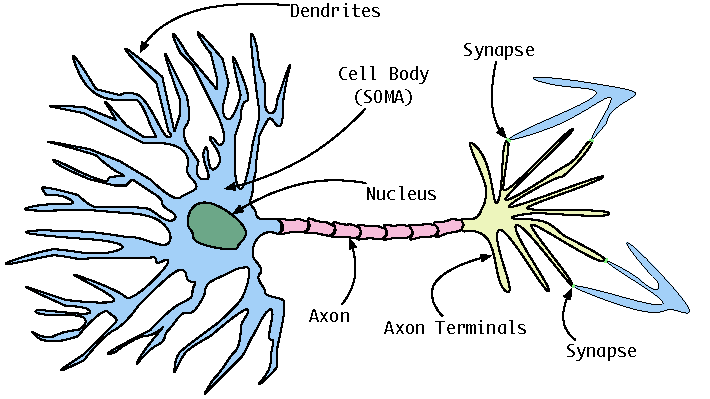
\includegraphics[width=4.0in]{Neuron.pdf}}
}
\caption{Artist's impression of a mammalian neuron \cite{wikipedia_neuron}}
\label{fig:neuron}
\end{figure}



\iftrue
It is known that mammalian neurons generate ``spikes'' in response to inputs that for humans include sight, touch, sound etc.. This spiking behavior is often referred to as the neuron being activated.
When these neurons are activated, their spikes propagate to other neurons. Under certain conditions, the combination of the various inputs to a neuron causes it to activate. 
A particular neuron may have many hundreds, perhaps thousands of other neurons connected to its ``input.''
These input neurons are referred to as pre-synaptic neurons. These pre-synaptic neurons may provide input to many neurons that are referred to as post-synaptic neurons.
A particular neuron can get activated by a particular arrival pattern of pre-synaptic neuron spikes or simply by the intensity of the pre-synaptic spikes. 

The spiking behavior of a neuron also varies and many spiking profiles have been observed, including single spikes, groups of spikes and repetitive spiking. 
It is believed that information is carried in the delay and strength of the connections and how pre-synaptic neurons combine to cause a neuron to activate.
In simple terms, if a neuron is activated by its pre-synaptic neurons, then the activation of the neuron means a pattern has been detected which will influence a reaction.
In mammalian terms, that might be the detection of a threat from both smell and sight neurons and the reaction is to control muscles resulting in flight.


The various chemical and electrical processes that result in the generation and propagation of these neuron spikes is beyond the scope of this dissertation, but how neurons and networks of neurons are artificially emulated is what we will discuss next.


%\section[NnSP]{NnSP{\cite{esmaeilzadeh2005nnsp}}}
\subsection[ANN Overview]{ANN Overview}
\label{sec:ANN Overview}

When modeling these neurons in artificial neural networks, the neuron models either generate actual spikes similar to actual neurons or
produce a value that is proportional to the rate at which spikes occur.
These \acp{ann} can be categorized as rate-based coded or spike time coded neurons \cite{10.3389/fnsys.2015.00151}\cite{NNintro_Bullinaria}.


When used in networks of neurons, both model types employ a connection weight between the pre and post-synaptic neuron.
However, the spiking neuron network also introduces a time delay associated with the connection.

The spiking neuron model \cite{paugam2012computing} is characterized by:
\vspace{-3mm}
\begin{outline}
  %\setlength{\baselineskip}{10pt}
  %\setlength{\itemsep}{12pt}
  %\setlength{\partopsep}{0pt}
  %\setlength{\parskip}{0pt}
  %\setlength{\parsep}{0pt}
  %\setlength{\topsep}{0pt}
  %\setlength{\itemindent}{\leftmargin}
  %\setlength{\leftmargin}{0pt}
        %\1 Connections between neurons have both a strength and a delay
        \1 Connections have a strength and a delay
\vspace{-3mm}
         % \2 The pre-synaptic neuron output is multiplied by the connection weight and delayed 
        \1 The weighted inputs from all pre-synaptic neurons are accumulated
\vspace{-3mm}
        \1 The accumulated inputs drive an activation function
\vspace{-3mm}
%          \2 the activation function $f(x)$ is a spiking model based on differential equations
          \2 The activation function $f(x)$ is based on differential equations
          \2 Varying levels of complexity from Leaky integrate and fire \cite{Brunel2007} to Izhikevich \cite{Iz2005} (see \fref{fig:Izhikevich Model})
          %\2 many models have been proposed with varying levels of complexity
              %\3 from Leaky integrate and fire \cite{Brunel2007} to Izhikevich \cite{Iz2005} (see \fref{fig:Izhikevich Model})
              %\3 complexity based on the number of differential equations and/or computations
         
\end{outline}

The Rate-based neuron model \cite{NNintro_Bullinaria} is characterized by:
\vspace{-3mm}
\begin{outline}
        \1 Connections between neurons have only a strength
\vspace{-3mm}
          %\2 The pre-synaptic neuron output is multiplied by the connection weight
        \1 The weighted inputs from all pre-synaptic neurons are accumulated
\vspace{-3mm}
        \1 The accumulated inputs drive a differentiable non-linear activation function $f(x)$
\vspace{-3mm}
          \2 Such as Sigmoid \cite{paugam2012computing} or \ac{relu} \cite{maas2013rectifier} (see \fref{fig:Example Rated-Based Model Activation functions}):
          %\2 the activation function $f(x)$ is a non-linear function
          %\2 early models used binary functions although in practice the function needs to be differentiable
            %\3 examples are (see \fref{fig:Example Rated-Based Model Activation functions}):
              %\4 sigmoid \cite{paugam2012computing} \ac{relu} \cite{maas2013rectifier}
\end{outline}

\begin{figure}
\centering
\begin{subfigure}{.4\textwidth}
  \centering
  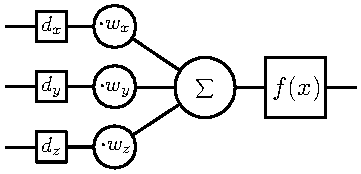
\includegraphics[width=0.85\textwidth]{SpikeBasedModel}
  \captionsetup{justification=centering, skip=5pt}
  \caption[Spiking Model]{Spiking Model}
  \label{fig:Spiking Model}
\end{subfigure}%
\begin{subfigure}{.4\textwidth}
  \centering
  \includegraphics[width=0.7\textwidth]{RatebasedModel}
  \captionsetup{justification=centering, skip=5pt}
  \caption{Rate-Based Model}
  \label{fig:Rate Based Model}
\end{subfigure}
\begin{subfigure}{.9\textwidth}
  \centering
  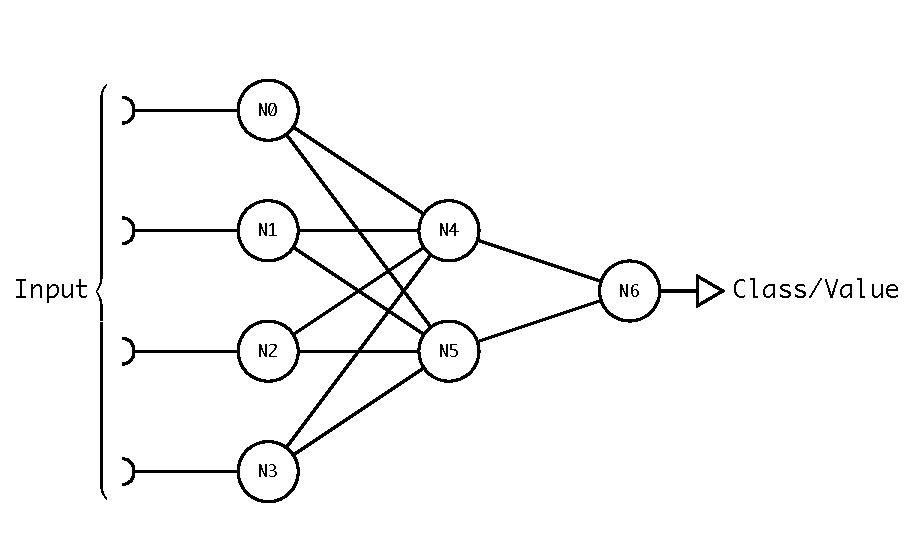
\includegraphics[width=0.7\textwidth]{SimpleNetwork}
  \captionsetup{justification=centering, skip=5pt}
  \caption{Network of Artificial Neurons}
  \label{fig:Network of ANs}
\end{subfigure}
\captionsetup{justification=centering, skip=6pt}
\caption[Artificial Neural Network]{Artificial Neurons and Network \cite{NNintro_Bullinaria}\cite{NNintro_Nielsen}}
\label{fig:Artificial Neural Network}
\end{figure}

\begin{figure}
\centering
\begin{subfigure}{.3\textwidth}
  \begin{tikzpicture}[scale=0.5]
    \begin{axis}[
        title={Sigmoid},
        %grid = major,
        xmin=-6,xmax=6,
        ymin=0,ymax=1,
        legend style={draw=none, fill=white},      
        legend pos= outer north east
        ]
        \addplot[myBlueThickStyle] expression[domain=-6:6,samples=100]{1/(1+e^(-x))} 
                    node at (axis cs:3,0.7){}; 
        \legend{{\large $f(x)=\frac{1}{1+e^{-x}}$}}
    \end{axis}
  \end{tikzpicture}
  \captionsetup{justification=centering, skip=5pt}
  \caption{Sigmoid \cite{paugam2012computing}}
  \label{fig:Sigmoid}
\end{subfigure}%
\begin{subfigure}{.3\textwidth}
  \begin{tikzpicture}[scale=0.5]
    \begin{axis}[
        title={ReLu},
        xmin=-1,xmax=1,
        ymin=0,ymax=1,
        legend style={draw=none, fill=white},      
        legend pos= outer north east
        ]
        \addplot[myBlueThickStyle] expression[domain=0:1,samples=100]{x} node at (axis cs:0.6,0.15){}; 
         \addplot[myBlueThickStyle] expression[domain=-1:0,samples=100]{0};       
         % had to change , to f&%$$#$g \text{,} on max.ece.ncsu.edu, what BS
         \legend  {{ $f(x)= \begin{cases} 0\text{,}      &\text{if $x < 0$;}\\   x\text{,}       &\text{otherwise.}  \end{cases}$}}  
    \end{axis}
  \end{tikzpicture}
  \captionsetup{justification=centering, skip=5pt}
  \caption{\ac{relu} \cite{maas2013rectifier} }
  \label{fig:Relu}
\end{subfigure}
\captionsetup{justification=centering, skip=5pt}
\caption{Example Rated-Based Model Activation functions}
\label{fig:Example Rated-Based Model Activation functions}
\end{figure}

\begin{figure}
\centering
\captionsetup{justification=centering}
\vspace{0.5cm}
\begin{subfigure}{.9\textwidth}
  \centering
  \begin{equation}
    \begin{split}
    &v' = 0.04v^2+5v + 140 - u - I\\
    &u' = a(bv-u)  \\
    &\text{if } v\ge  \SI{30}{\mV}, \text{ then } 
    \begin{cases}
        v \leftarrow c\\           
        u \leftarrow u+d\\           
    \end{cases} \nonumber
    \end{split}
  \end{equation}
  \caption{Izhikevich Model\cite{Iz2005}}
  \label{fig:Izhikevich Model}
  \end{subfigure}
\begin{subfigure}{.7\textwidth}
  \centering
  \mbox{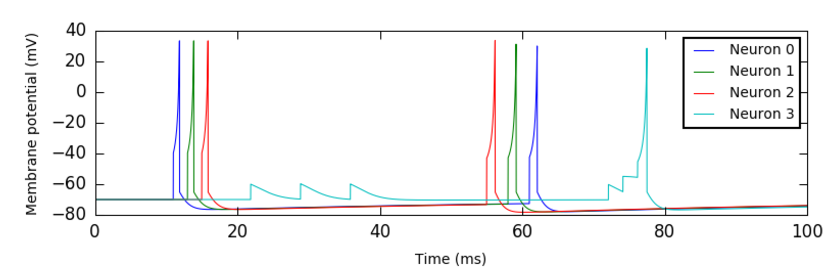
\includegraphics[width=4.0in]{SpikingExample.pdf}}
  \captionsetup{justification=centering, skip=3pt}
  \caption{Izhikevich Model Simulation \cite{carnevale2006neuron}\cite{Iz2005}}
  \label{fig:spiking example}
\end{subfigure}
\caption{Example Spiking Activation Function Model}
\label{fig:Example Spiking Model}
\end{figure}

The artificial neurons are connected in networks, typically with layers of sub-networks which are in effect separated by the non-linear activation function, to emulate complex behavior.
Examples of both rate-based and spiking artificial neural networks can be seen in \fref{fig:Rate-based Model Network} and \fref{fig:Spiking Model Network} respectively.
Typically neural networks process in a feed-forward fashion. Considering \fref{fig:Network of ANs}, this means the input arrives on the left, the inputs propagate to neurons N0 through N3. 
When N0 through N3 are processed, their values propagate forward to neurons N4 and N5 etc.. Sometimes \ac{ann}s also include recursion where for example neurons N0 through N4 are not only influenced
by the input, but also by themselves. Many \ac{ann}s operate only in feed-forward fashion but some popular \ac{ann}s, such as \ac{lstm} \cite{hochreiter1997long}, employ recursion.

Another popular type of \ac{ann}, the \ac{dnn} \cite{aizenberg2013multi}\cite{doi:10.1162/neco.2006.18.7.1527} has gained traction over the last few years. \acp{dnn} get good press in applications such as image recognition and speech recognition. 
\acp{dnn} are often formed from tens of layers of \ac{an}s with each layer containing many \ac{an}s. \ac{dnn}s are also processed in a feed-forward manner with one layer being the inputs to the next layer. 
As mentioned in \cite{krizhevsky2012imagenet}, these useful \ac{dnn}s often require hundreds of thousands of \ac{an}s and within the network, each \ac{an} can have hundreds, even thousands of feeder or pre-synaptic \ac{an}s.
There have been implementations that use different number formats from double precision floating point to eight bit integers, but in all cases, these useful \ac{ann}s require a significant amount of memory to store the connection weights (parameters).


\begin{figure}[!t]
  % the [] contains position info e.g. [!t] means here
  \centering
  \captionsetup{justification=centering}
  \captionsetup{width=.9\linewidth}
  \begin{subfigure}{.9\textwidth}
    \centerline{
    \mbox{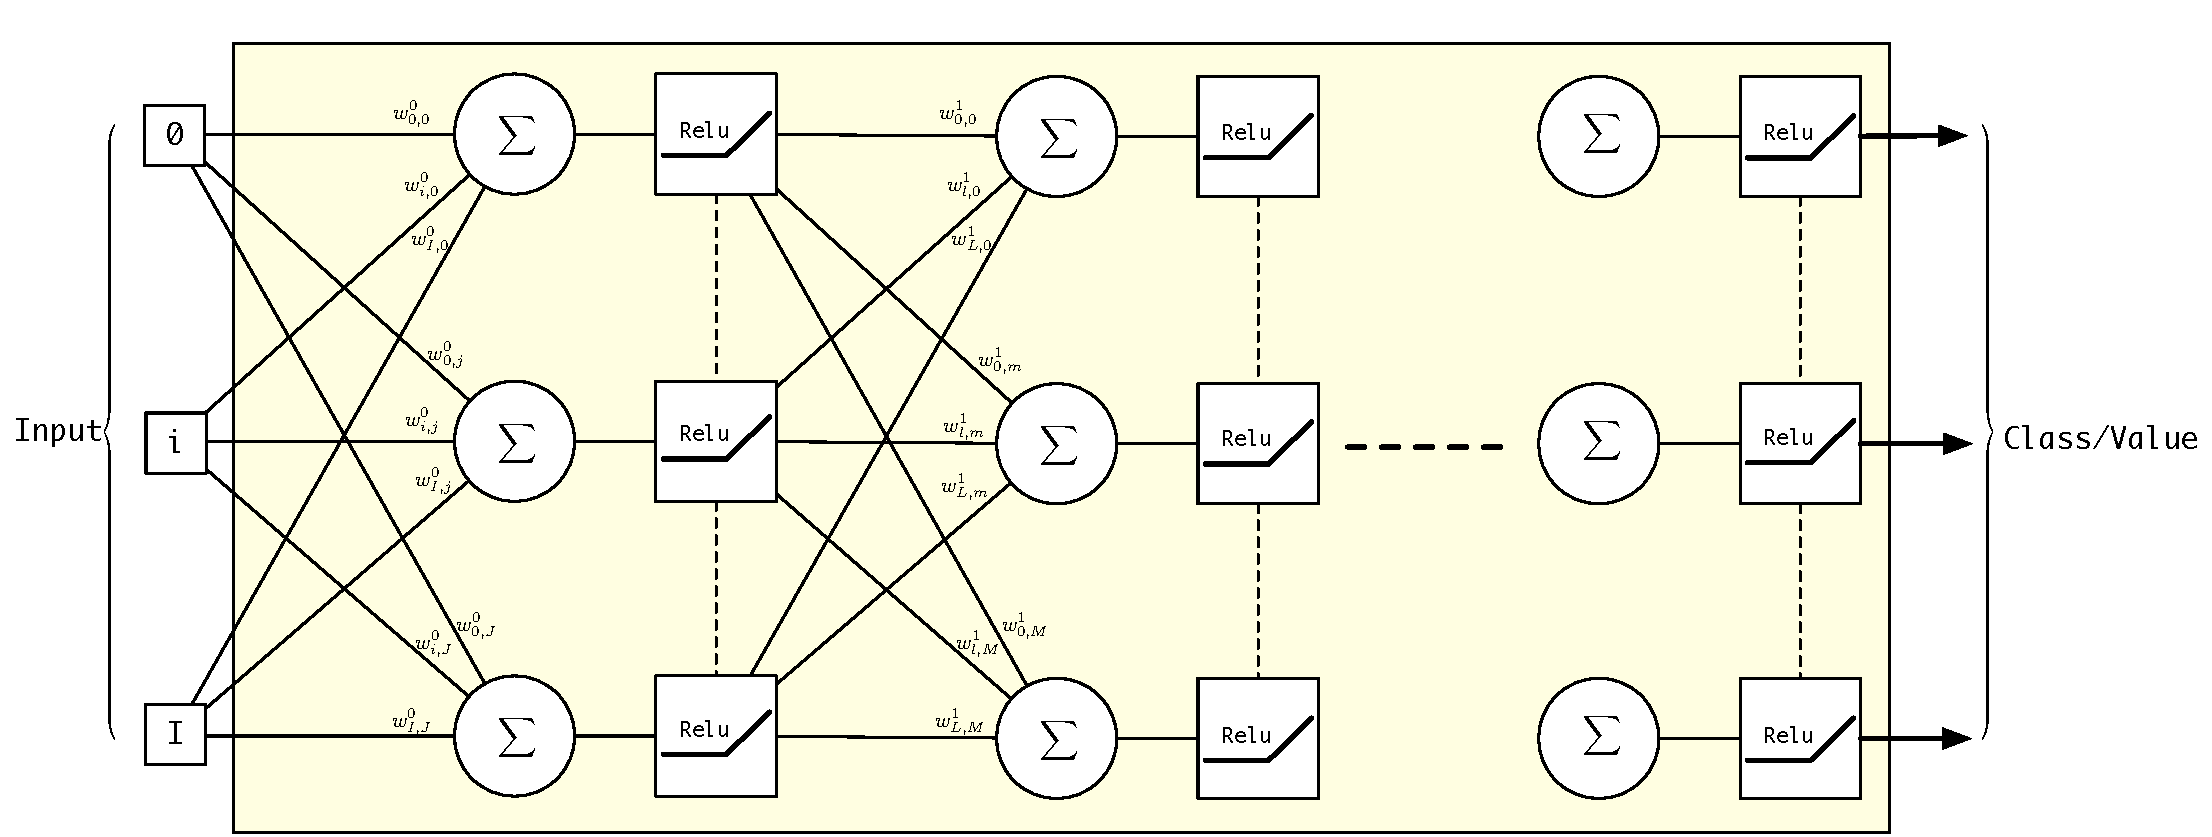
\includegraphics[width=0.85\textwidth]{RateBasedNeuralNetwork.pdf}}
    }
    \caption{Rate-based Model Artificial Neural Network (with ReLu activation function)}
    \label{fig:Rate-based Model Network}
  \end{subfigure}
  
  \begin{subfigure}{.9\textwidth}
    \centerline{
    \mbox{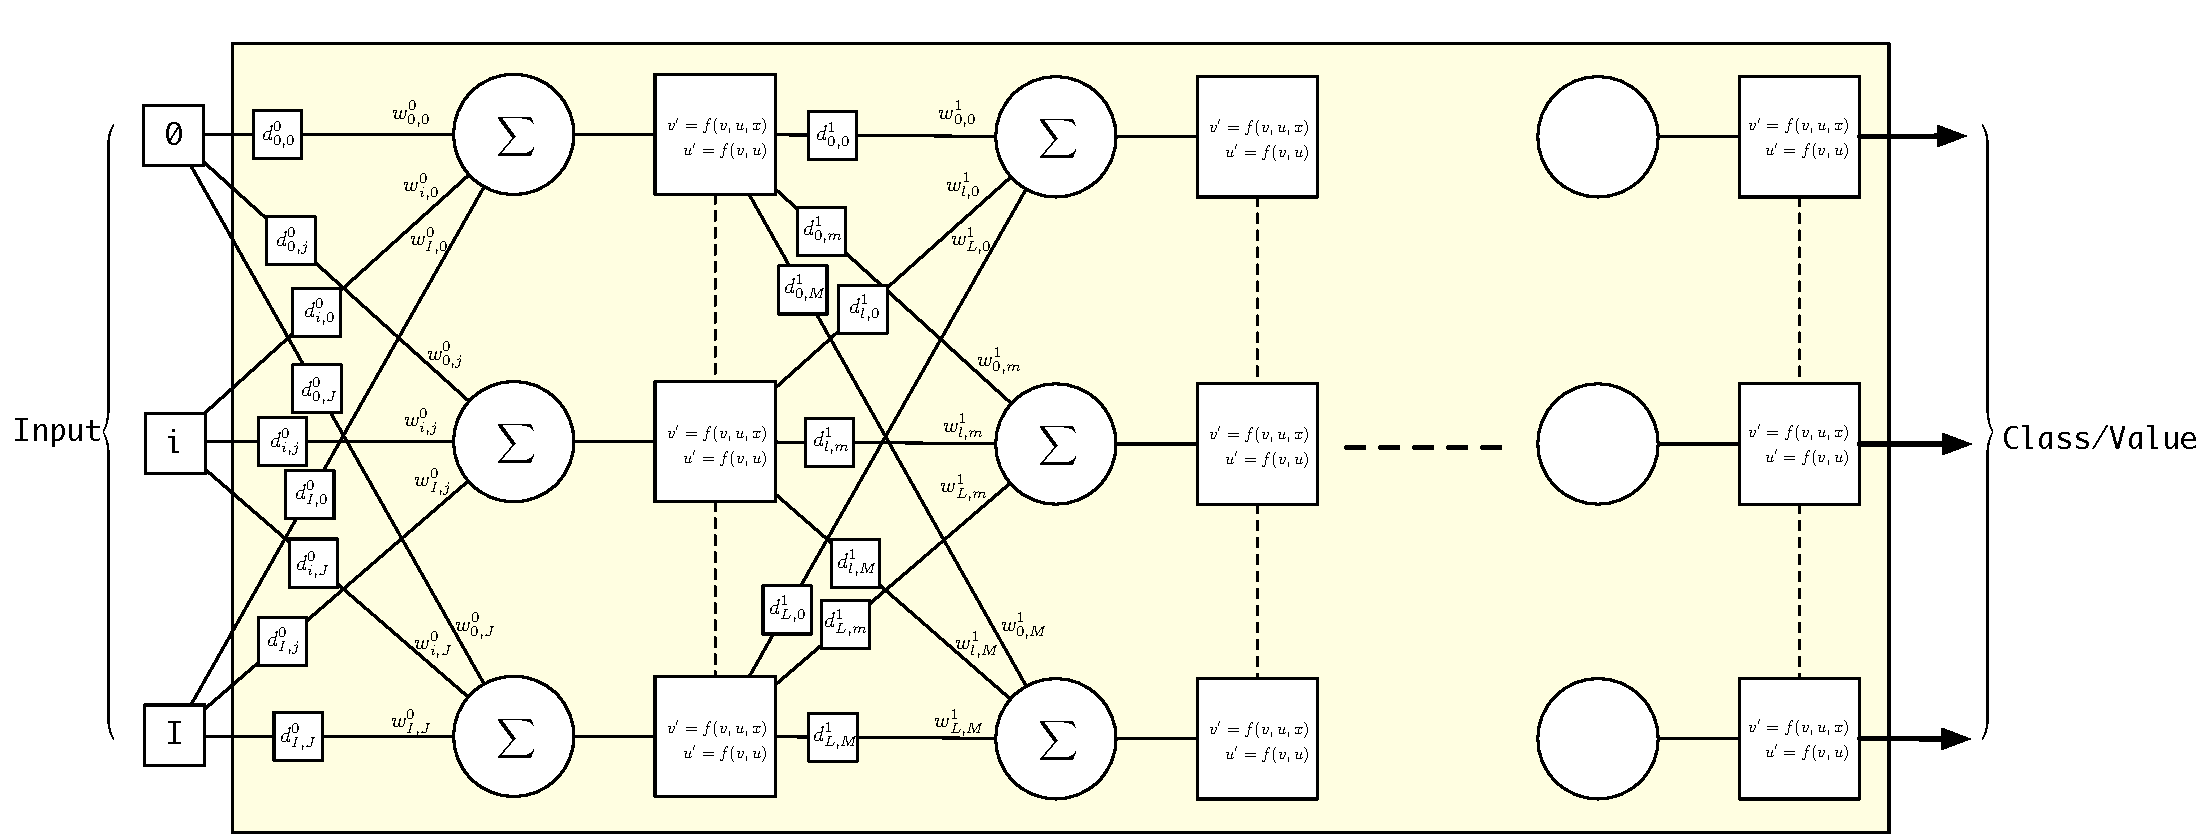
\includegraphics[width=0.85\textwidth]{SpikingNeuralNetwork.pdf}}
    }
    \caption{Spiking-based Model Artificial Neural Network}
    \label{fig:Spiking Model Network}
  \end{subfigure}
  \caption{Layered Artificial Neural Networks}
  \label{fig:Layered Artificial Neural Networks}
\end{figure}

Although the spiking neural network more closely models the behavior of real neurons, over the last 20 years there 
have been breakthroughs in the ``teaching'' of rate-based models, especially with the introduction of the back-propagation algorithm \cite{wikipedia_back_propagation} and stochastic gradient descent \cite{wikipedia_sgd} which are used to ``learn'' the connection weights of a \ac{dnn}. 
Along with the abundance of data now available in the form of voice, images etc. to ``teach'' these networks using back-propagation, most of the effective applications of \acp{ann} have employed these rate-based models.

\iffalse
Our research will focus on these rate-based models which we will now refer to as \ac{ann}s.
\fi

This work does not address the training or ``teaching'' of these rate-based \acp{ann}.
The training is mostly performed offline. 
This work is addressing inference using \acp{ann} where the \acp{ann} are used for example to detect objects in an image or reproduce the output of a cost function based on the observed values.
During inference, the most computationally intensive operation is the multiply-accumulate associated with the \ac{an} activation, which can involve hundreds or thousands of multiply-accumulates.
The \ac{an} activation calculation for the rate-based \ac{an} in Figure \ref{fig:Rate Based Model} is shown in \eqref{eq:activation function}.

\begin{alignat}{2} 
\label{eq:activation function}
\text{\ac{an} activation }\hspace{4mm} A & = f\bigg(\sum_{n=0}^{C_n}W_n \mathbf{\cdot} A_n\bigg)  \\
              &\mathbf{C_n} \text{ is the number of pre-synaptic connections} \notag\\
              &\mathbf{W_n} \text{ is the weight of a connection} \notag\\
              &\mathbf{A_n} \text{ is the state of the pre-synaptic \ac{an}} \notag \\
\text{and }   &f(x) \text{ is the activation function such as \ac{relu} \cite{maas2013rectifier}}  \notag 
\end{alignat}

\subsection[ANN Layers]{ANN Layers}
\label{sec:ANN Layers}

In Figure \ref{fig:Network of ANs} and \ref{fig:Rate-based Model Network}, the \ac{ann} is shown to be constructed using layers of \acp{an}. 
%It has long been known that a single layer of \acp{an} can be used to linearly partition an n-dimensional input \cite{NNintro_Bullinaria}, as shown in Figure \ref{fig:linear discrimination}.
It has long been known that a single layer of \acp{an} can be used to partition an n-dimensional input \cite{NNintro_Bullinaria} using a linear combination of the inputs, as shown in Figure \ref{fig:linear discrimination}.
%However, if a more complex partition is required, this cannot be achieved using a single layer of \acp{an}. 
However, a more complex partition, as shown in Figure \ref{fig:complex discrimination}, can only be achieved using multiple layers of \acp{an}. 
%A higher order classification where the , as shown in Figure \ref{fig:complex discrimination} can only be achieved using multiple layers of \acp{an}. 
To ensure the multiple layers cannot be mathematically collapsed into a single layer, the activation function $f(x)$, as shown in Figure \ref{fig:Rate Based Model} must be a non-linear function.



\begin{figure}[h]
\centering
  \begin{subfigure}{.4\textwidth}
    \centering
    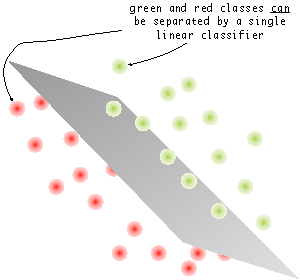
\includegraphics[width=0.85\textwidth]{linearDiscrimination}
    \captionsetup{width=.8\textwidth, justification=centering, skip=20pt}
    \caption{Linear Classification using a single layer}
    \label{fig:linear discrimination}
  \end{subfigure}%
  \begin{subfigure}{.4\textwidth}
    \centering
    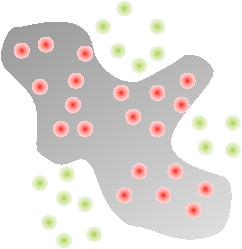
\includegraphics[width=0.7\textwidth]{complexDiscrimination}
    \captionsetup{width=.8\textwidth, justification=centering, skip=10pt}
    \caption{Complex Classification requires multiple layers}
    \label{fig:complex discrimination}
  \end{subfigure}
\captionsetup{justification=centering, skip=10pt}
\caption{Classification using \acp{ann} layers \cite{NNintro_Bullinaria}}
\label{fig:Discrimination}
\end{figure}


\subsubsection{Deep Neural Networks}
\label{sec:Deep Neural Networks}

As mentioned, a single layer of neurons can be used as a linear classifier as long as the classes can be separated using a linear function.
Even some simple cases cannot be linearly separated, an example often used is an exclusive-OR gate \cite{NNintro_Bullinaria}.

Even with a layered \ac{ann}, the final output comes from a single layer. To allow this final layer to linearly separate classes, the original input needs to be transformed into a space where the classes can be linearly separated.
\acfp{dnn} are \acp{ann} that incorporate many layers of \acp{an}, often that are tens of layers deep.
The additional layers are incorporated to translate the space of the input so the various classes being identified can be separated using linear classifiers in the later layers.

Recently, an example of a \ac{dnn} known as a \acf{cnn} demonstrated high levels of efficacy when used to classify objects in images \cite{krizhevsky2012imagenet}.
These \acp{cnn} use the early layers to identify low-level features and later layers are used combine these features into yet more high-level features \cite{deeplearning4j}\cite{Kwolek2005}\cite{wikipedia_deep_learning}.
Finally, the combination of high-level features is used to identify the required classes.
This layering is shown in \fref{fig:Deep network showing feature layers}.
\begin{figure}[h]
\centering
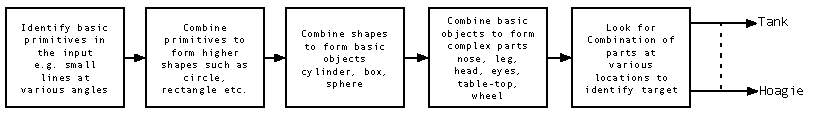
\includegraphics[width=0.95\textwidth]{deepNetworkBlockDiagram}
\captionsetup{justification=centering, skip=5pt}
\caption{Deep network showing feature layers}
\label{fig:Deep network showing feature layers}
\end{figure}

In figure \ref{fig:Deep network showing feature layers}, the final layer is often a fully connected linear classifier with the output representing the probability of a particular class being present in the image.
In practice, these \acp{dnn} can be used as classifiers or as function approximators.

\iffalse
In practice, useful deep neural networks are very large and often exceed the capacity of single GPUs. Therefore,  there is opportunity for a solution that provides
real-time acceleration and storage of of these systems.
\fi


\subsubsection{Feature Layers}
\label{sec:Feature Layers}

For the most part, different \acp{ann} are characterized by how the \acp{an} are interconnected and the activation function employed.

The typical \ac{dnn} layers are processed in a feed-forward fashion where the pre-synaptic \acp{an} are formed from \acp{an} in the previous layer.
There are some types of \ac{dnn} that also include recursive connections where the pre-synaptic \acp{an} include \acp{an} from the current layer.
A popular recursive \ac{dnn} is \acf{lstm} \cite{hochreiter1997long}. Although this work does not preclude supporting \ac{lstm} in the future, the focus of this work is on the feed-forward type \ac{dnn}.

As described in Section \ref{sec:Deep Neural Networks}, a \ac{dnn} layer transforms the previous layer with each higher layer providing a coarser grained transformation. 
This is best seen in image recognition applications, where the early layers identify low-level shapes or features, such as angled lines. 
The following layers are used to identify higher order shapes such as circles, blocks etc. 
Although the features detected during the image recognition application are somewhat intuitive, it is believed that in less intuitive applications the \ac{dnn} performs a similar fine to coarse feature extraction.

The connections between layers can be locally- or fully-connected. 
With locally-connected layers as shown in Figure \ref{fig:Locally Connected Layer to Layer Connection Types}, a layer's pre-synaptic \acp{an} are formed from regions of the previous layer.
With fully-connected layers as shown in Figure \ref{fig:Fully Connected Layer to Layer Connection Types}, a layers pre-synaptic \acp{an} are formed from all \acp{an} in the previous layer.
In many cases, a \ac{dnn} is constructed with lower layers being locally-connected and higher layers being fully-connected \cite{krizhevsky2012imagenet}.

\begin{figure}[h]
  \centering

  \begin{subfigure}{1.0\textwidth}
    \centering
    \begin{subfigure}{.5\textwidth}
      \centering
      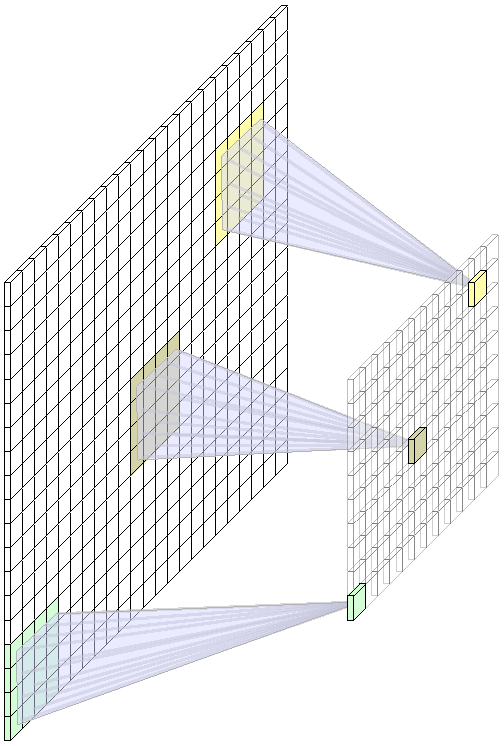
\includegraphics[width=0.50\textwidth]{localArrayToArrayConnections}
      \captionsetup{width=.8\textwidth, justification=centering, skip=10pt}
      \caption{Local Array to Array}
      \label{fig:Local Array to Array}
    \end{subfigure}%
    \begin{subfigure}{.5\textwidth}
      \centering
      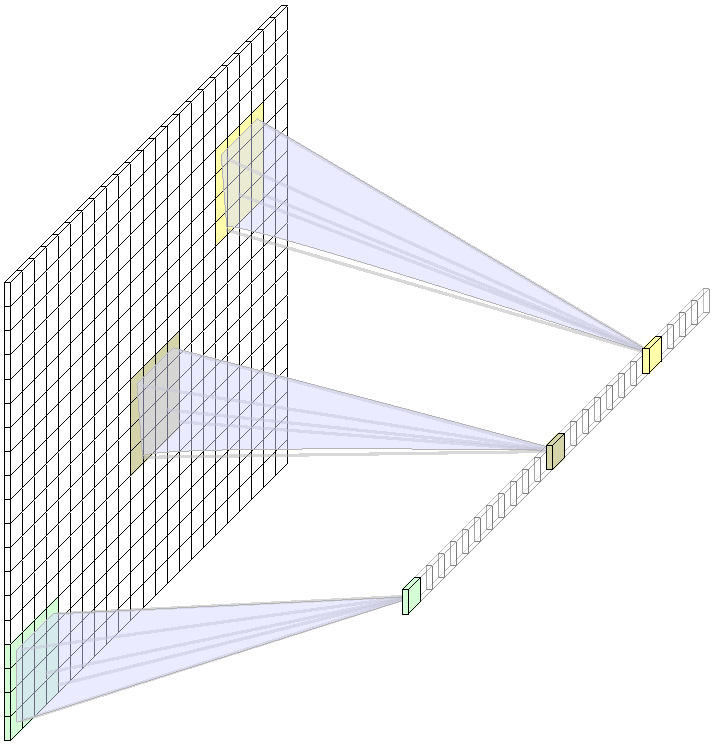
\includegraphics[width=0.70\textwidth]{localArrayToLinearConnections}
      \captionsetup{width=.8\textwidth, justification=centering, skip=10pt}
      \caption{Local Array to Linear}
      \label{fig:Local Array to Linear}
    \end{subfigure}
  \end{subfigure}

  \bigskip

  \begin{subfigure}{1.0\textwidth}
    \centering
    \begin{subfigure}{.5\textwidth}
      \centering
      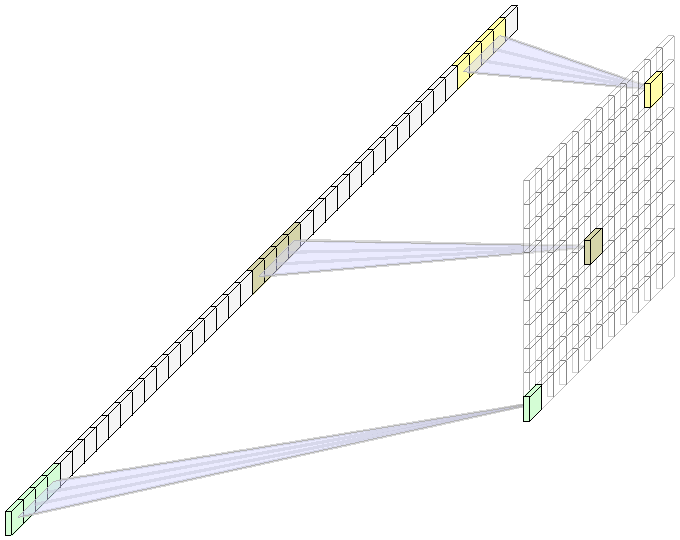
\includegraphics[width=0.60\textwidth]{localLinearToArrayConnections}
      \captionsetup{width=.8\textwidth, justification=centering, skip=10pt}
      \caption{Local Linear to Array}
      \label{fig:Local Linear to Array}
    \end{subfigure}%
    \begin{subfigure}{.5\textwidth}
      \centering
      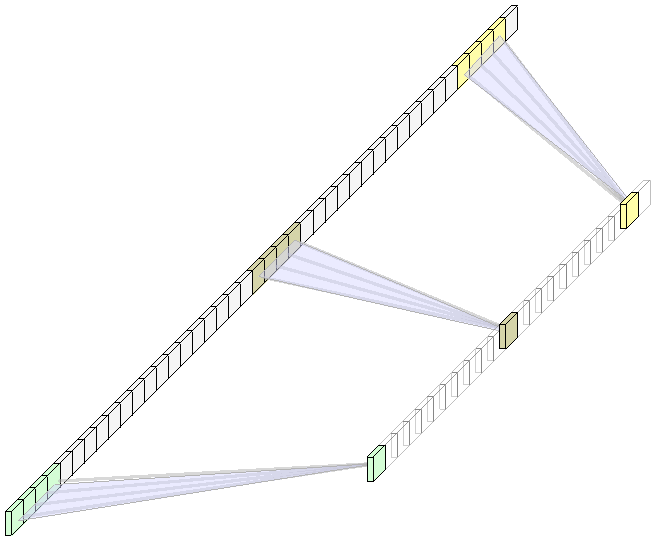
\includegraphics[width=0.60\textwidth]{localLinearToLinearConnections}
      \captionsetup{width=.8\textwidth, justification=centering, skip=10pt}
      \caption{Local Linear to Linear}
      \label{fig:Local Linear to Linear}
    \end{subfigure}
  \end{subfigure}

\captionsetup{justification=centering, skip=10pt}
\caption{Locally Connected Layer to Layer Connection Types}
\label{fig:Locally Connected Layer to Layer Connection Types}
\end{figure}

\begin{figure}[h]
  \centering
  \begin{subfigure}{1.0\textwidth}
    \centering
    \begin{subfigure}{.5\textwidth}
      \centering
      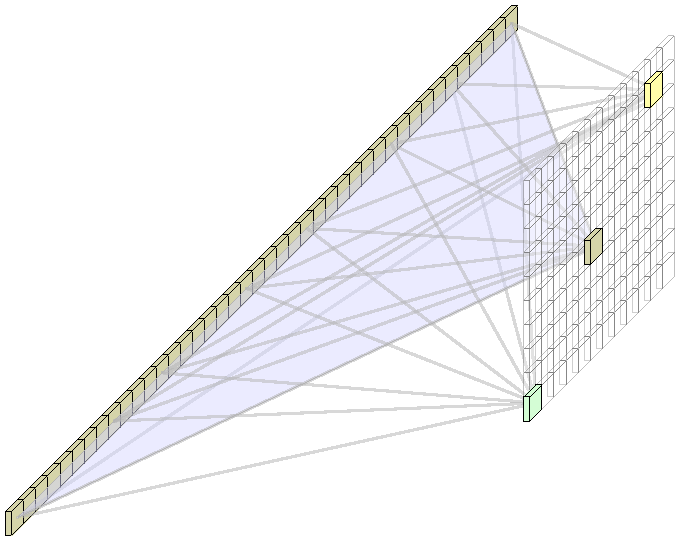
\includegraphics[width=0.60\textwidth]{fullLinearToArrayConnections}
      \captionsetup{width=.8\textwidth, justification=centering, skip=10pt}
      \caption{Full Linear to Array}
      \label{fig:Full Linear to Array}
    \end{subfigure}%
    \begin{subfigure}{.5\textwidth}
      \centering
      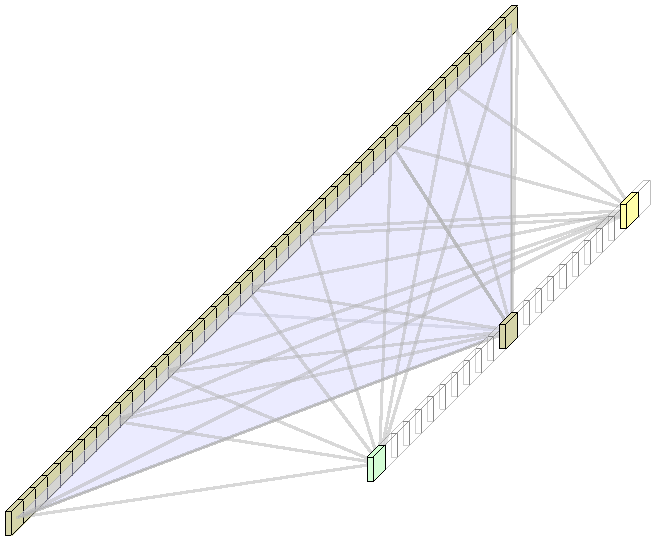
\includegraphics[width=0.60\textwidth]{fullLinearToLinearConnections}
      \captionsetup{width=.8\textwidth, justification=centering, skip=10pt}
      \caption{Full Linear to Linear}
      \label{fig:Full Linear to Linear}
    \end{subfigure}
  \end{subfigure}

  \bigskip

  \begin{subfigure}{1.0\textwidth}
    \centering
    \begin{subfigure}{.5\textwidth}
      \centering
      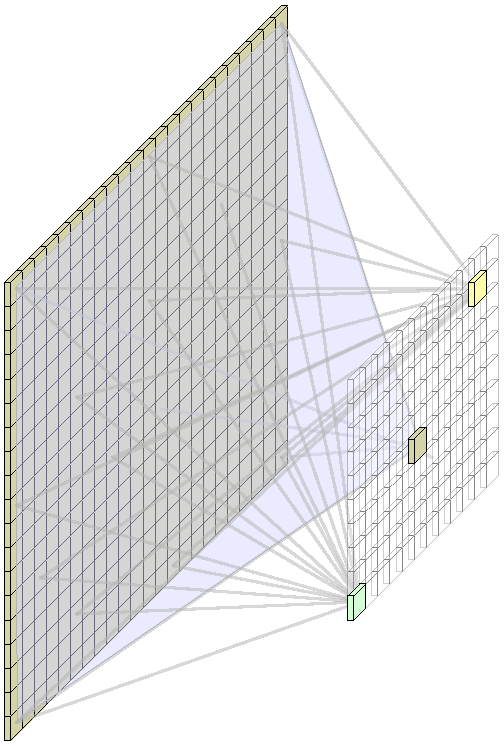
\includegraphics[width=0.50\textwidth]{fullArrayToArrayConnections}
      \captionsetup{width=.8\textwidth, justification=centering, skip=10pt}
      \caption{Full Array to Array}
      \label{fig:Full Array to Array}
    \end{subfigure}%
    \begin{subfigure}{.5\textwidth}
      \centering
      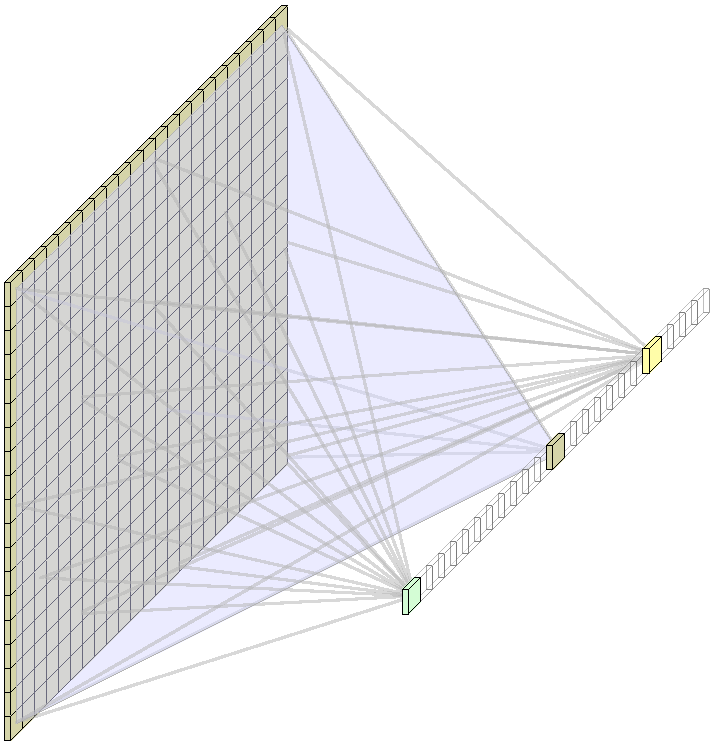
\includegraphics[width=0.7\textwidth]{fullArrayToLinearConnections}
      \captionsetup{width=.8\textwidth, justification=centering, skip=10pt}
      \caption{Full Array to Linear}
      \label{fig:Full Array to Linear}
    \end{subfigure}
  \end{subfigure}

\captionsetup{justification=centering, skip=10pt}
\caption{Fully Connected Layer to Layer Connection Types}
\label{fig:Fully Connected Layer to Layer Connection Types}
\end{figure}

\iffalse With locally-connected layers, the connection weights of the pre-synaptic \acp{an} are often formed from wanting to identify particular features. \fi
In early uses of locally-connected \acp{ann}, the first layers weights were often hand-generated, an example being Gabor filters \cite{Kwolek2005}. 
With automatically trained \acp{ann}, the feature detectors at each layer are often created during training.
Some contrived examples of locally-connected feature detectors are shown in Figure \ref{fig:Features and locally-connected filters (kernels)}.
\begin{figure}[h]
\centering
  %\begin{subfigure}{.7\textwidth}
    %\centering
    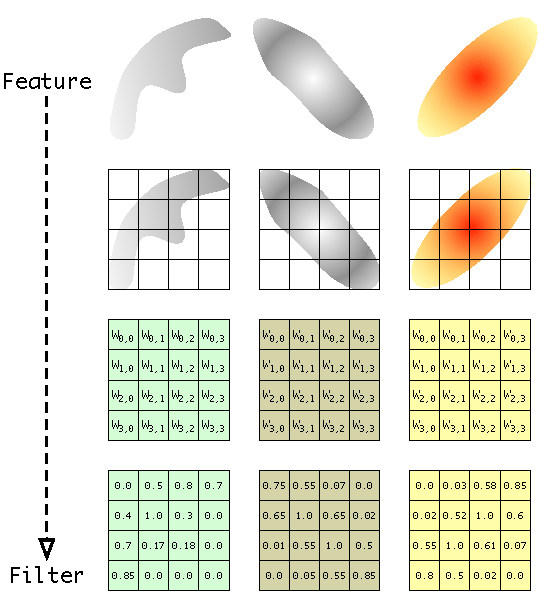
\includegraphics[width=0.55\textwidth]{locallyConnectedFeatures}
    \captionsetup{justification=centering, skip=5pt}
    \caption{Features and locally-connected filters (kernels)}
    \label{fig:Features and locally-connected filters (kernels)}
  %\end{subfigure}%
\end{figure}

The pre-synaptic \acp{an} of a locally-connected \ac{an} are formed from a particular \ac{roi} of the previous layer using the weights from a feature filter. 
Another locally-connected \ac{an} may use the same \ac{roi} but employs a different filter.
In practice, for a particular \ac{roi}, a number of feature filters are employed resulting in a number of \acp{an} being associated with the same \ac{roi} in the previous layer. 
To reiterate, these feature filters all operate on the same \ac{roi}.
A different \ac{roi} will result in another group of \acp{an} all using their own feature filters.
The resulting locally-connected layer becomes a \ac{3d} layer with its X-Y coordinates representing a reference to a particular \ac{roi} and the Z-dimension representing the various filters applied to that \ac{roi}.
An example \ac{3d} locally-connected layer can be seen in Figure \ref{fig:3D layers of Features}.

\iffalse
A good example of the feature filters is image recognition \acp{ann}. The lower level features generated during automatic training are often intuitive and the filters are constructed to detect small features such as lines at various angles, different curves etc..
In the general \ac{dnn} case, the trained feature detectors may not be as intuitive.
\fi
  %\bigskip

\begin{figure}[h]
\centering
  %\begin{subfigure}{.7\textwidth}
    %\centering
    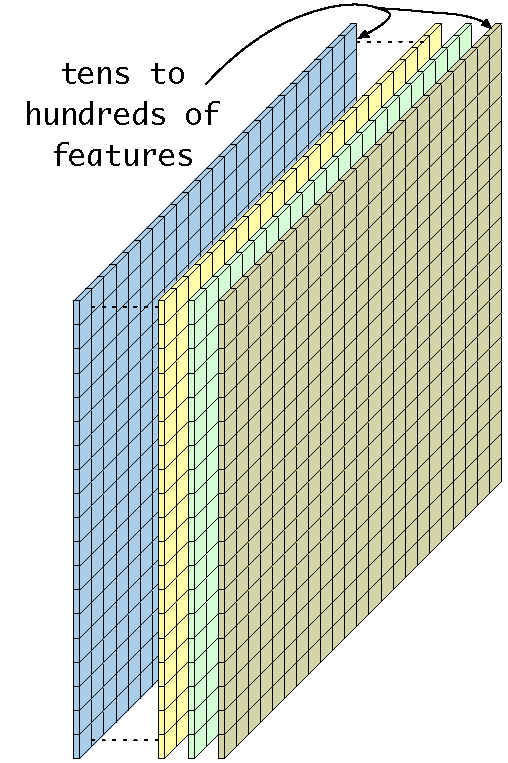
\includegraphics[width=0.35\textwidth]{layer3DFeatures}
    \captionsetup{justification=centering, skip=5pt}
    \caption{Single Layer constructed from 3D layers of Features}
    \label{fig:3D layers of Features}
  %\end{subfigure}
%\captionsetup{justification=centering, skip=10pt}
%\caption{Layer Feature Planes}
\label{fig:Layer Features}
\end{figure}

%%\begin{figure}[h]
%%\centering
%%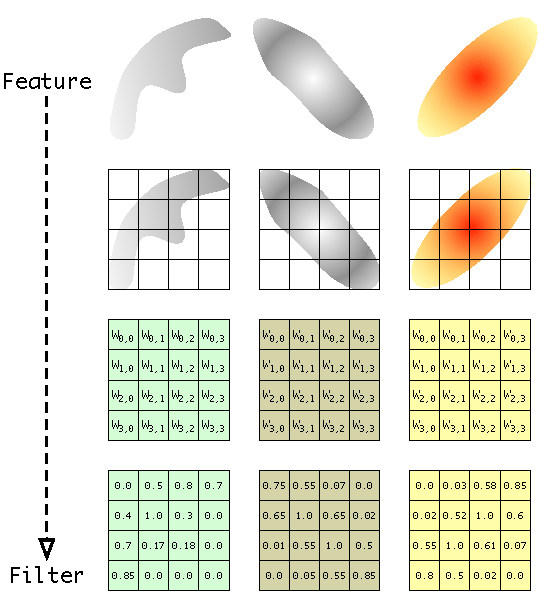
\includegraphics[width=0.55\textwidth]{locallyConnectedFeatures}
%%\captionsetup{justification=centering, skip=5pt}
%%\caption{Features and locally-connected filters (kernels)}
%%\label{fig:Features and locally-connected filters (kernels)}
%%\end{figure}
%%
%%\begin{figure}[h]
%%\centering
%%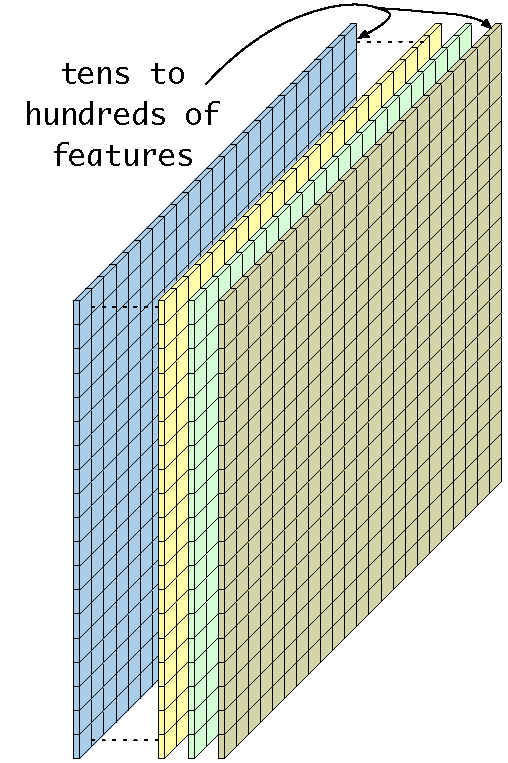
\includegraphics[width=0.55\textwidth]{layer3DFeatures}
%%\captionsetup{justification=centering, skip=5pt}
%%\caption{Features form 3D layers}
%%\label{fig:Features form 3D layers}
%%\end{figure}

So these locally-connected layers have multiple filters applied to the same \ac{roi} and the next layer becomes a \ac{3d} array with the Z-axis representing the features. 
The number of feature filters applied at each layer can be tens to hundreds of filters.
The filters employed in a layer following one of these \ac{3d} locally-connected layers are themselves 3D. With tens to hundreds of features in the previous layer the number of weights associated with each filter is usually hundreds to thousands of weights. 

The feature filters employed in the locally-connected layers can be unique to the regions of the previous layer or the same filters can be employed across the entire previous layer.
In the case of employing the same filters across the entire input layer the \ac{ann} is known as a \acf{cnn}. 
The \acp{cnn} are examples of \acp{ann} that can take advantage of reuse. % described in Chapter \ref{sec:chap-one}. 
These \acp{cnn} can store the filter parameters in local \ac{sram} and construct an entire feature plane. These \acp{cnn} are considered a subset of the generic case of \ac{dnn}.
This work considers the more general \ac{dnn} case and supports acceleration of generic \acp{dnn} that includes \acp{cnn}.

An example of a \ac{dnn} can be seen in Figure \ref{fig:Baseline DNN showing layer order} with the layer configurations shown in Table \ref{tab:Baseline Layer Configuration}. 
A \ac{cnn} similar to this has demonstrated high levels of efficacy in image recognition applications.
{\textbf{\textcolor{black}{Therefore, this work will use the parameters from Table \ref{tab:Baseline Layer Configuration} as a template for a baseline \ac{ann} for estimating the storage and processing requirements and the range of pre-synaptic fanins.}}}

%%


%%%% \begin{sidewaysfigure}[h]
%%%%   %\begin{adjustbox}{angle=0, width=1.0\textwidth}
%%%%     \centering
%%%%     \captionsetup{justification=centering}
%%%%     \begin{subtable}{.9\textwidth}
%%%%       %\captionsetup{justification=centering, skip=-5pt}
%%%%       \centering
%%%%       %\begin{center}
%%%%        % [lr] ~ left align col 0 and right align col 1
%%%%        % e.g. 4 columns could be lccr
%%%%       \begin{adjustbox}{width=1\textwidth}
%%%%         \begin{tabular}{|r|c|c|c|c|c|c|c|c|c|c|c|c|c}\cline{3-13}
%%%%           %\toprule
%%%%            \multicolumn{2}{c|}  {\multirow{2}{*}{}}    & \multicolumn{11}{c|}{Layers}    \\\cline{3-13}
%%%%            \multicolumn{2}{c|}{}                       &  1 & 2 & 3 & 4 & 5 & 6 & 7 & 8 & 9 & 10 & 11  \\\cline{3-13} \cline{1-13}
%%%%            \multicolumn{2}{|r|}{Type}                  &  Input          & Locally      & Pooling           & Locally             & Pooling             & Locally             & Locally             & Locally             &  Fully              &  Fully                 &  Fully         &                                    \\\cline{1-13}
%%%%            \multirow{3}{*}{Dimensions}               &X& \num{       256}& \num{     55}& \num{    27}      & \num{     27}       & \num{     13}       & \num{     13}       & \num{     13}       & \num{     13}       & \num{      4096}    & \num{     4096}        & \num{    1024} &                                    \\
%%%%                                                      &Y& \num{       256}& \num{     55}& \num{    27}      & \num{     27}       & \num{     13}       & \num{     13}       & \num{     13}       & \num{     13}       & \num{         1}    & \num{        1}        & \num{       1} &                                    \\
%%%%                                                      &Z& \num{         3}& \num{     96}& \num{    96}      & \num{    256}       & \num{    256}       & \num{    384}       & \num{    384}       & \num{    256}       & \num{         1}    & \num{        1}        & \num{       1} &                                    \\\cline{1-13}
%%%%            \multirow{3}{*}{Filter Dimensions}        &X&    na           & \num{     11}& \num{     2}      & \num{      5}       & \num{      2}       & \num{      3}       & \num{      3}       & \num{      3}       & \num{        13}    & \num{     4096}        & \num{    4096} &                                    \\
%%%%                                                      &Y&    na           & \num{     11}& \num{     2}      & \num{      5}       & \num{      2}       & \num{      3}       & \num{      3}       & \num{      3}       & \num{        13}    & \num{        1}        & \num{       1} &                                    \\
%%%%                                                      &Z&    na           & \num{      3}& \num{     1}      & \num{     96}       & \num{      1}       & \num{    256}       & \num{    384}       & \num{    384}       & \num{       256}    & \num{        1}        & \num{       1} &                                    \\\cline{1-14}
%%%%             \multicolumn{2}{|r|}{Stride           }    &    na           & \num{      4}& \num{     2}      & \num{      2}       & \num{      2}       & \num{      1}       & \num{      1}       & \num{      1}       &              na     &             na         &            na  & \multicolumn{1}{c|}{Aggregate    } \\\cline{14-14}
%%%%             \multicolumn{2}{|r|}{Pre-synaptic Fanin}   &    na           & \num{    363}& \num{     4}      & \num{   2400}       & \num{      4}       & \num{   2304}       & \num{   3456}       & \num{   3456}       & \num{     43264}    & \num{     4096}        & \num{    4096} & \multicolumn{1}{c|}{$\Bar{\num{   1650}}$} \\
%%%%             \multicolumn{2}{|r|}{Number of \ac{an}}    & \num{    196608}& \num{ 290400}& \num{ 69984}      & \num{ 186624}       & \num{  43264}       & \num{  64896}       & \num{  64896}       & \num{  43264}       & \num{      4096}    & \num{     4096}        & \num{    1024} & \multicolumn{1}{c|}{\num{ 772544}} \\
%%%%             \multicolumn{2}{|r|}{Number of Weights}    &    na           & \num{  34848}& na                & \num{ 614400}       & na                  & \num{ 884736}       & \num{ 1327104}      & \num{ 884736}       & \num{ 177209344}    & \num{ 16777216}        & \num{ 4194304} & \multicolumn{1}{c|}{\num{ 2.02e8}} \\\hline
%%%%         \end{tabular}
%%%%       \end{adjustbox}
%%%%       \captionsetup{justification=centering, skip=9pt}
%%%%       \vspace{0.5cm}
%%%%       \caption{Baseline \ac{ann} Layer Configuration \cite{krizhevsky2012imagenet}}
%%%%       \label{tab:Layer Configuration}
%%%%       %  \end{center}
%%%%     \end{subtable}
%%%%   
%%%%     \bigskip
%%%% 
%%%%     %\begin{adjustbox}{width=1.0\textwidth}
%%%%       \begin{subfigure}{1\textwidth}
%%%%         \centering
%%%%         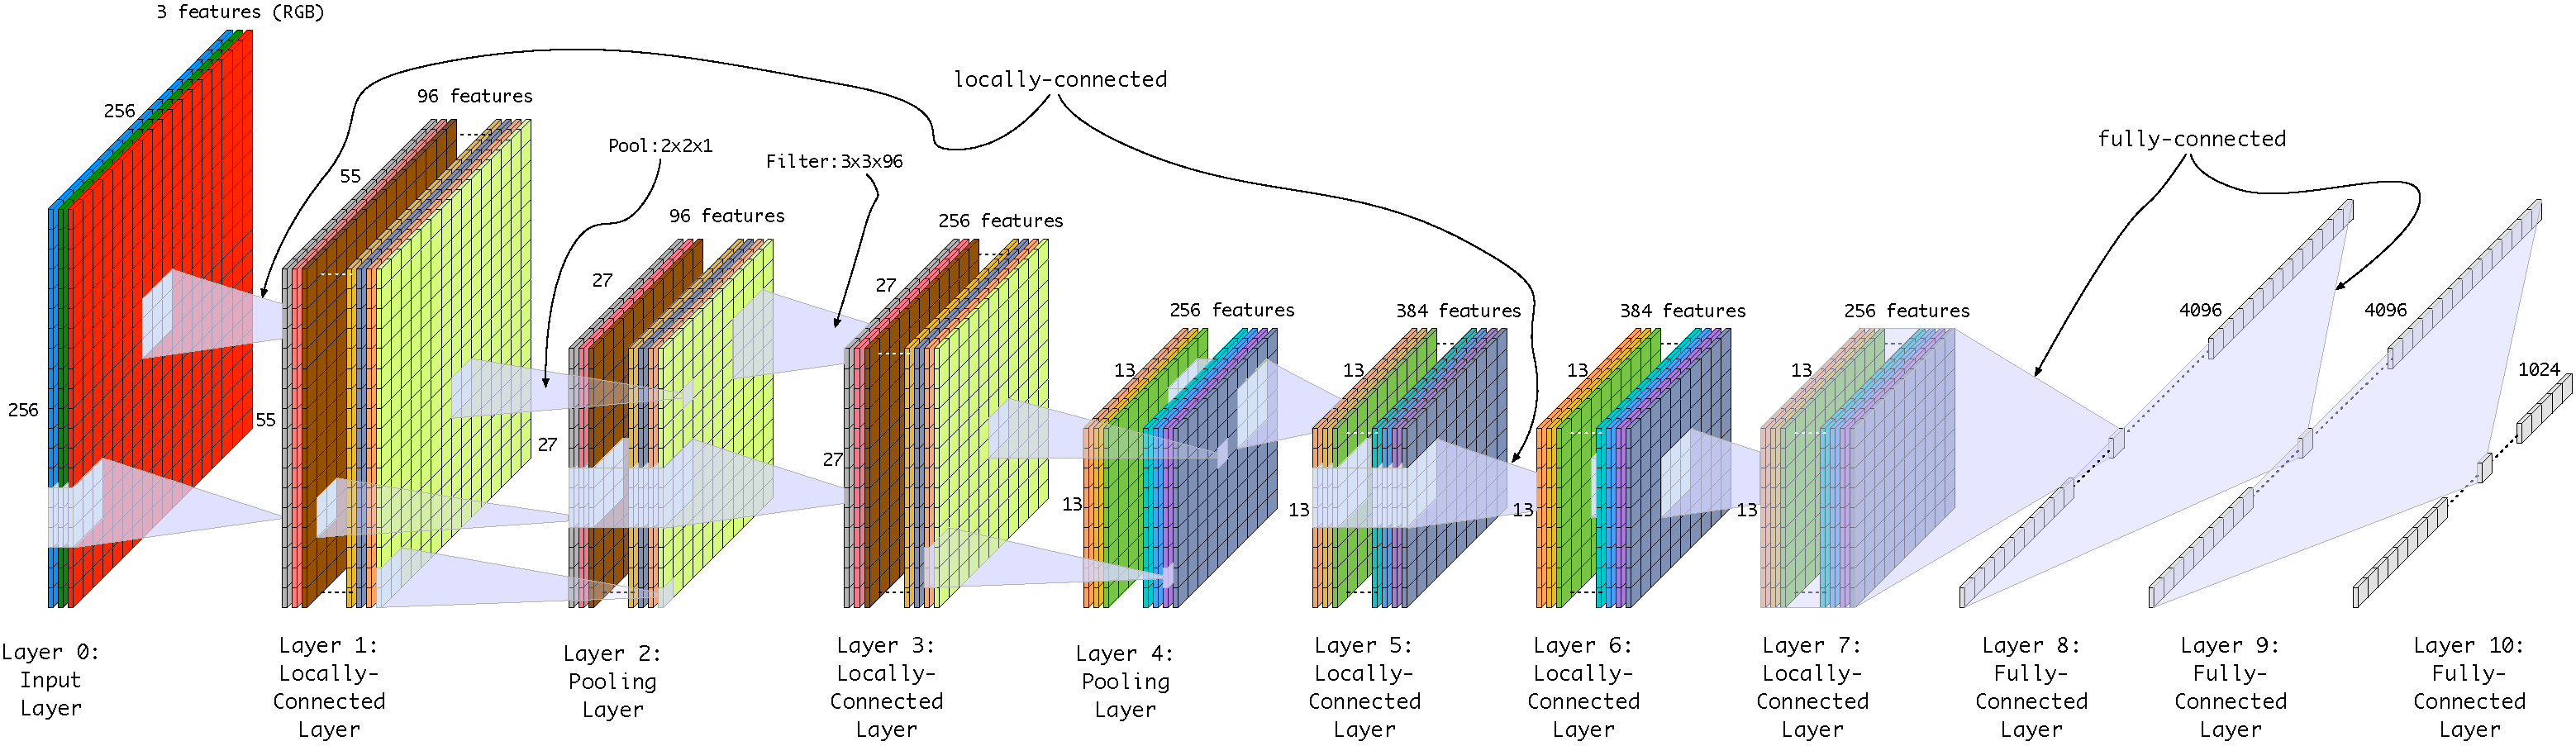
\includegraphics[width=1.0\textwidth]{fullDNN}
%%%%         \captionsetup{justification=centering, skip=15pt}
%%%%         \caption{DNN showing layer order \cite{krizhevsky2012imagenet}}
%%%%         \label{fig:DNN showing layer order}
%%%%       \end{subfigure}
%%%%     %\end{adjustbox}
%%%%   
%%%%   %\end{adjustbox}
%%%%   \caption{Baseline DNN \cite{krizhevsky2012imagenet}}
%%%%   \label{fig:Baseline DNN}
%%%% \end{sidewaysfigure}


\begin{sidewaysfigure}[!htbp]
  %\begin{adjustbox}{angle=0, width=1.0\textwidth}
    \centering
    \captionsetup{justification=centering}
    \begin{minipage}{.9\textwidth}
      %\captionsetup{justification=centering, skip=-5pt}
      \centering
      %\begin{center}
       % [lr] ~ left align col 0 and right align col 1
       % e.g. 4 columns could be lccr
      \begin{adjustbox}{width=1\textwidth}
        \begin{tabular}{|r|c|c|c|c|c|c|c|c|c|c|c|c|c}\cline{3-13}
          %\toprule
           \multicolumn{2}{c|}  {\multirow{2}{*}{}}    & \multicolumn{11}{c|}{Layers}    \\\cline{3-13}
           \multicolumn{2}{c|}{}                       &  1 & 2 & 3 & 4 & 5 & 6 & 7 & 8 & 9 & 10 & 11  \\\cline{3-13} \cline{1-13}
           \multicolumn{2}{|r|}{Type}                  &  Input          & Locally      & Pooling           & Locally             & Pooling             & Locally             & Locally             & Locally             &  Fully              &  Fully                 &  Fully         &                                    \\\cline{1-13}
           \multirow{3}{*}{Dimensions}               &X& \num{       256}& \num{     55}& \num{    27}      & \num{     27}       & \num{     13}       & \num{     13}       & \num{     13}       & \num{     13}       & \num{      4096}    & \num{     4096}        & \num{    1024} &                                    \\
                                                     &Y& \num{       256}& \num{     55}& \num{    27}      & \num{     27}       & \num{     13}       & \num{     13}       & \num{     13}       & \num{     13}       & \num{         1}    & \num{        1}        & \num{       1} &                                    \\
                                                     &Z& \num{         3}& \num{     96}& \num{    96}      & \num{    256}       & \num{    256}       & \num{    384}       & \num{    384}       & \num{    256}       & \num{         1}    & \num{        1}        & \num{       1} &                                    \\\cline{1-13}
           \multirow{3}{*}{Filter Dimensions}        &X&    na           & \num{     11}& \num{     2}      & \num{      5}       & \num{      2}       & \num{      3}       & \num{      3}       & \num{      3}       & \num{        13}    & \num{     4096}        & \num{    4096} &                                    \\
                                                     &Y&    na           & \num{     11}& \num{     2}      & \num{      5}       & \num{      2}       & \num{      3}       & \num{      3}       & \num{      3}       & \num{        13}    & \num{        1}        & \num{       1} &                                    \\
                                                     &Z&    na           & \num{      3}& \num{     1}      & \num{     96}       & \num{      1}       & \num{    256}       & \num{    384}       & \num{    384}       & \num{       256}    & \num{        1}        & \num{       1} &                                    \\\cline{1-14}
            \multicolumn{2}{|r|}{Stride           }    &    na           & \num{      4}& \num{     2}      & \num{      2}       & \num{      2}       & \num{      1}       & \num{      1}       & \num{      1}       &              na     &             na         &            na  & \multicolumn{1}{c|}{Aggregate    } \\\cline{14-14}
            \multicolumn{2}{|r|}{Pre-synaptic Fanin}   &    na           & \num{    363}& \num{     4}      & \num{   2400}       & \num{      4}       & \num{   2304}       & \num{   3456}       & \num{   3456}       & \num{     43264}    & \num{     4096}        & \num{    4096} & \multicolumn{1}{c|}{$\Bar{\num{   1650}}$} \\
            \multicolumn{2}{|r|}{Number of \ac{an}}    & \num{    196608}& \num{ 290400}& \num{ 69984}      & \num{ 186624}       & \num{  43264}       & \num{  64896}       & \num{  64896}       & \num{  43264}       & \num{      4096}    & \num{     4096}        & \num{    1024} & \multicolumn{1}{c|}{\num{ 772544}} \\
            \multicolumn{2}{|r|}{Number of Weights}    &    na           & \num{  34848}& na                & \num{ 614400}       & na                  & \num{ 884736}       & \num{ 1327104}      & \num{ 884736}       & \num{ 177209344}    & \num{ 16777216}        & \num{ 4194304} & \multicolumn{1}{c|}{\num{ 2.02e8}} \\\hline
        \end{tabular}
      \end{adjustbox}
      \captionsetup{justification=centering, skip=9pt}
      \vspace{0.5cm}
      \captionof{table}{Baseline \ac{ann} layer configuration \cite{krizhevsky2012imagenet}}
      \label{tab:Baseline Layer Configuration}
      %  \end{center}
    \end{minipage}
  
    \bigskip

    %\begin{adjustbox}{width=1.0\textwidth}
      \begin{minipage}{1\textwidth}
        \centering
        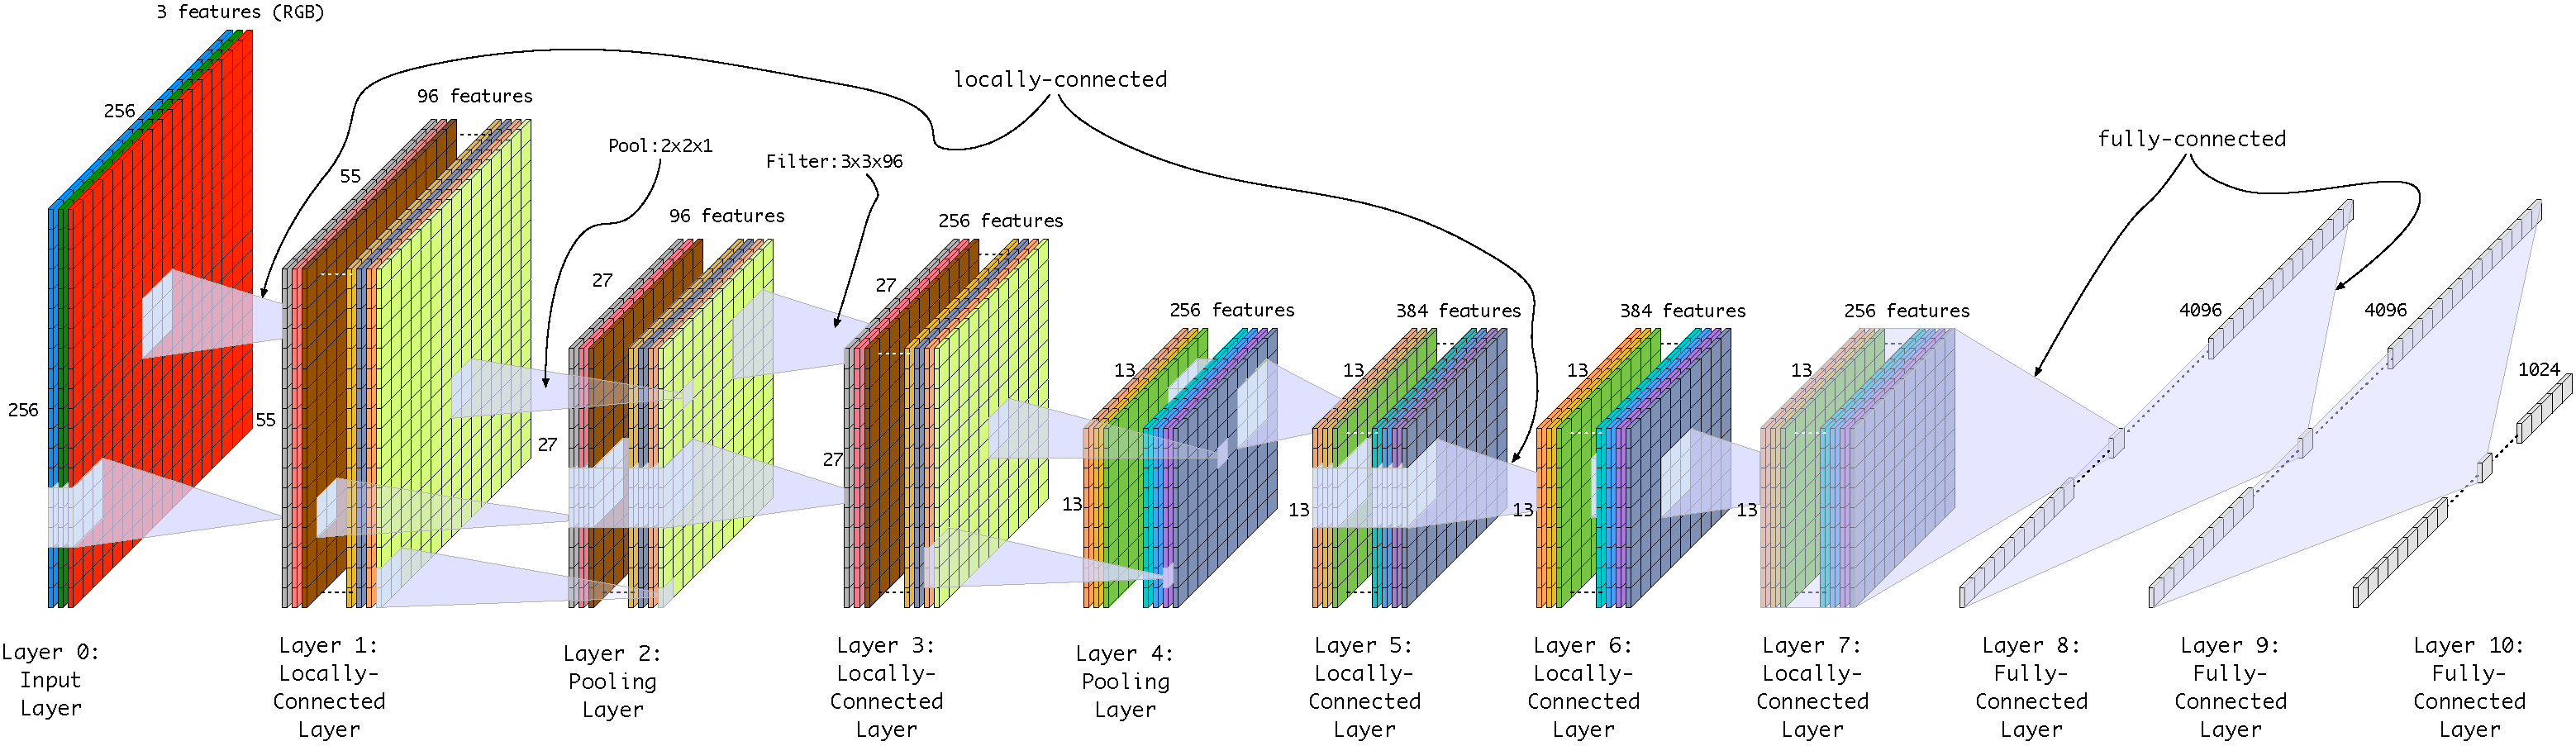
\includegraphics[width=1.0\textwidth]{fullDNN}
        \captionsetup{justification=centering, skip=15pt}
        \captionof{figure}{Baseline DNN showing layer order \cite{krizhevsky2012imagenet}}
        \label{fig:Baseline DNN showing layer order}
      \end{minipage}
    %\end{adjustbox}
  
  %\end{adjustbox}
  %\caption{Baseline DNN \cite{krizhevsky2012imagenet}}
  %\label{fig:Baseline DNN}
\end{sidewaysfigure}



\iffalse
\begin{sidewaysfigure}[h]
\centering
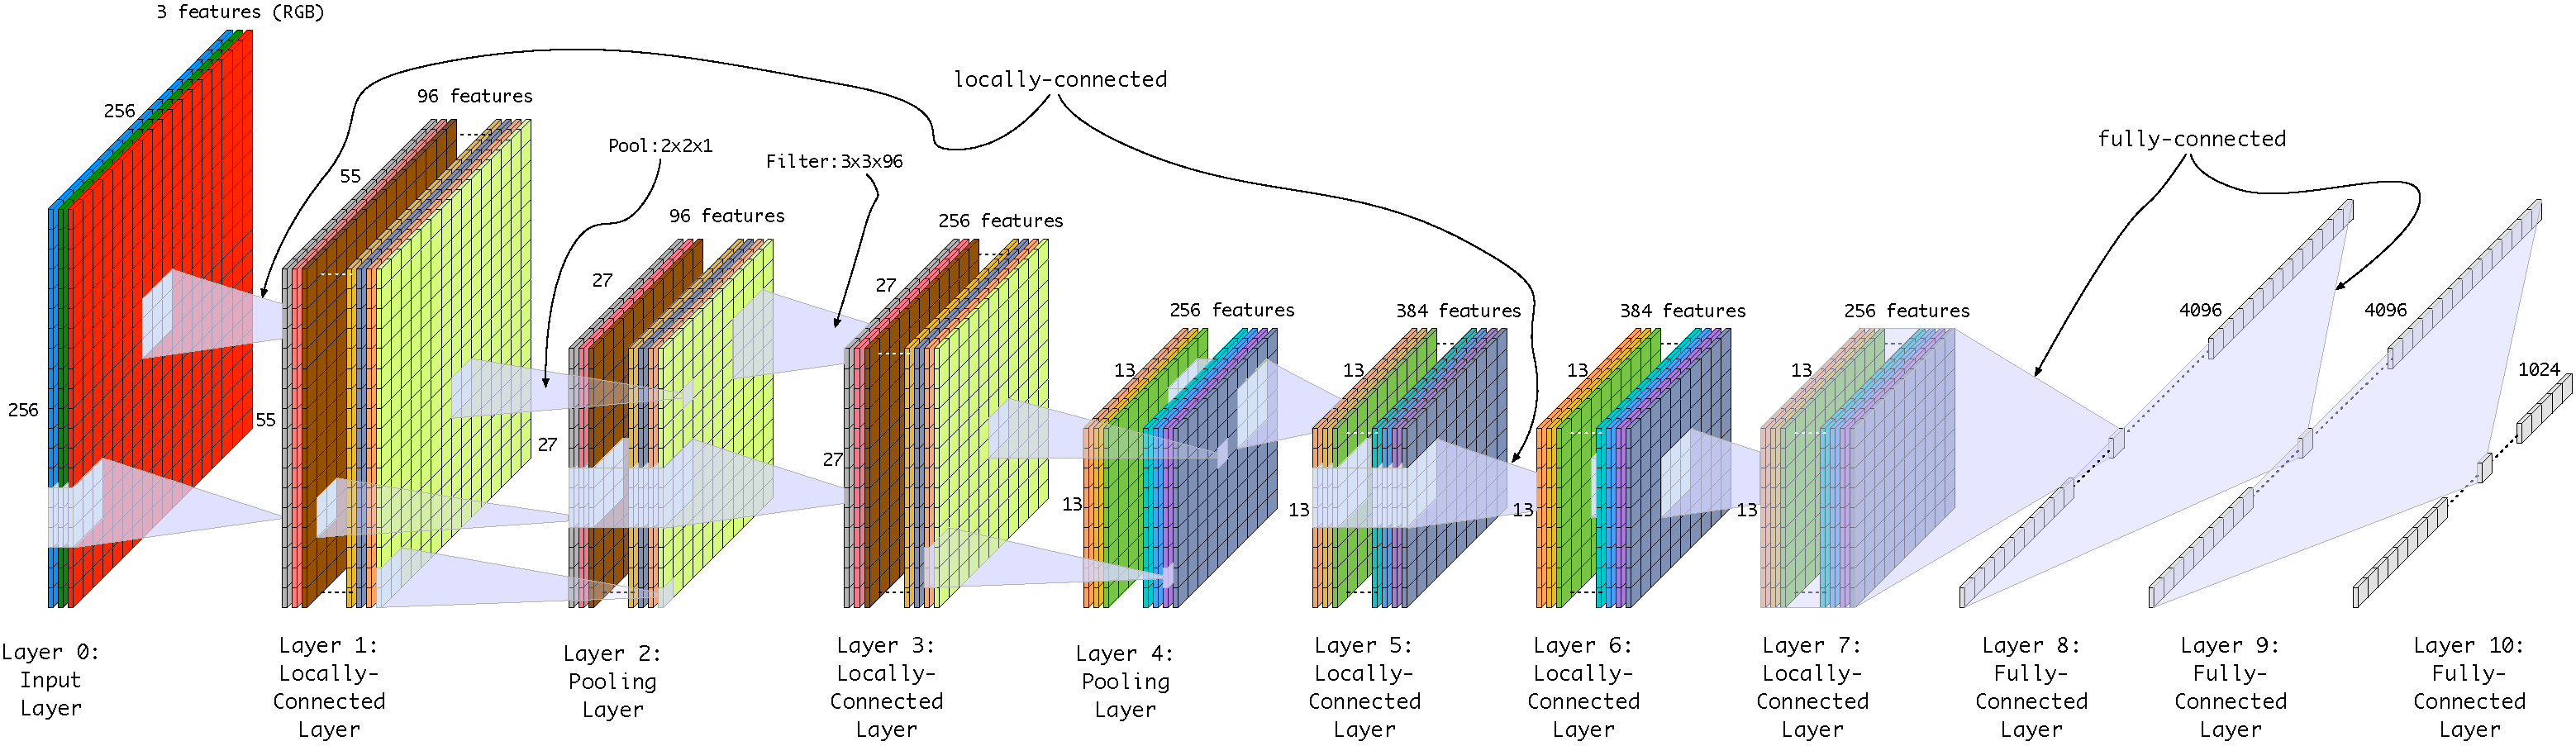
\includegraphics[width=1.0\textwidth]{fullDNN}
\captionsetup{justification=centering, skip=15pt}
\caption{DNN showing layer order \cite{krizhevsky2012imagenet}}
\label{fig:DNN showing layer order}
\end{sidewaysfigure}
\fi

To approach the capabilities observed in human behavior, such as object recognition, \ac{ann}s have become very large. 
The example shown in Figure \ref{fig:Baseline DNN showing layer order}, which is based on the work from \cite{krizhevsky2012imagenet}, has hundreds of thousands of \acp{an} and hundreds of millions of connection weights (see Table \ref{tab:Baseline Layer Configuration}).
These \acp{ann} utilize these hundreds of thousands of \acp{an} to implement what a human would consider a relatively straightforward task.
For example, a ``useful'' \ac{ann} similar to that described in \cite{krizhevsky2012imagenet} which was used to recognize up to 1000 different object classes, has a network size of approximately 650,000 \acp{an} and 630 million synaptic connections \cite{krizhevsky2012imagenetPreso}. 

The increased performance of \ac{ann}s over classical methods in image recognition and voice recognition might suggest that \ac{ann}s will out-perform operations performed in other applications.
\iffalse There is reason to believe that \acp{ann} will replace various functions in existing systems. \fi

If \acp{ann} fulfill their potential, systems employing \ac{ann}s will utilize them for various functions, such as engine monitoring, anomaly detection, navigation, etc., all within the same system.
Considering the various functions a complex customer facing or embedded application system performs, it is likely that many real-world applications will employ multiple disparate instances of these usefully sized \acp{ann}.
Assuming these complex functions will require \ac{ann}s similar in size to figure \ref{fig:Baseline DNN showing layer order} and \cite{krizhevsky2012imagenet}, these implementations will be processing multiple large \ac{ann}s at or near real-time.

\subsection[ANN Processing]{ANN Processing}
\label{sec:ANN Processing}

Considering the storage required for the input, the \ac{an} states and most significantly the weights for connections, the storage requirements results in gigabytes of memory.
When these \ac{ann}s are required to be solved in fractions of a second, the processing and memory bandwidth becomes prohibitive.

As a metric, this work assumes that any useful \ac{ann} will be similar to that shown in Table \ref{tab:Baseline Layer Configuration} which utilizes more than 900 thousand \acp{an} and approximately 200 million parameters. 
\iffalse
Given the bandwidth and storage requirements shown in Table \ref{tab:Bandwidth and Storage Design Requirements}, the problem becomes \hyphenquote{american}{\textbf{\textcolor{black}{to provide deterministic at or near real-time performance within tolerable power and space constraints for embedded systems employing inference on multiple disparate useful-sized neural networks.}}}
\fi
%\hlc[gray]{hello}
\iffalse
Considering that \ac{dram} is required to store the \ac{ann} parameters, why is it that much of the \ac{asic} and \ac{asip} \ac{ann} research employs \ac{sram} as an intermediate store? Well, in practice there are benefits if you can operate solely out of \ac{sram}.
Certainly good performance and potentially low power.
But use of \ac{sram} makes assumptions on the type of \acp{ann} that can be supported and the application in which the \ac{ann} is being deployed.
The primary requirement of the type of \ac{ann} and the deployed application to allow effective use of \ac{sram} is ``reuse.'' Reuse means that once parameters are transferred and stored in \ac{sram}, these parameters can be reused such that the \ac{sram} isn't simply an intermediate memory but something akin to a cache.

In some \ac{ann}s there are reuse opportunities. A prime example is \acp{cnn}, where the connection weights are reused. In \acp{cnn}, a common filter is passed across an input to form the next layer. These filter ``kernels'' can be held in memory and the input is read from \ac{dram} thus reducing the \ac{dram} bandwidth.
Even with \ac{dnn}s where weights may not be reused, when implementing multiple \ac{dnn}s, there is opportunity to hold the input in memory.
If the system is being employed in cloud applications or in training, there is opportunity to reuse inputs whilst performing batch processing.

But \ac{sram} comes at a price, its big. Often when we see physical layouts of \ac{ann} processors, they are dominated by the silicon area of the \ac{sram}. The area required for \ac{sram} can be prohibitive and companies attempt to create custom \acp{sram} to minimize the area impact.

So the question becomes, can a system employ \ac{dram} with minimal \ac{sram} and still provide a high performance system within acceptable area constraints?

\iffalse
We believe a system can be designed with \ac{dram} as the primary processing store. This will require careful use of data structures to describe storage within \ac{dram} to ensure we make good use of the potential bandwidth. But there are other benefits we will take advantage of, but more about that later.
\fi

\iffalse
There important application is disparate \ac{ann}s because specifically a form of \ac{dnn}, Convolutional Neural networks (\ac{cnn}) have gotten good press recently, but they are not the only \ac{dnn}.
\fi

Even in cloud applications, there are limitations on reuse. We paraphrase a quote from a Google paper \cite{jouppi2017datacenter} on their Tensor Processing Unit ASIC (TPU):

\hyphenquote{american}{the architecture research community is paying attention to \acp{ann}, but of all the papers at ISCA 2016 on hardware accelerators for \acp{ann}, alas, all nine papers looked at \ac{cnn}s, and only two mentioned other \acp{ann}. Unfortunately \ac{cnn}s represent only about 5\% of our datacenter \ac{ann} workload}

The applications targeted by the Google TPU \cite{jouppi2017datacenter} assume multiple requests, so reuse in the form of batch processing is still of great benefit, but the bulk of the requests in \cite{jouppi2017datacenter} are fully-connected \ac{dnn}s and in these cases weight reuse is not as beneficial and the performance of the TPU is degraded when implementing these fully-connected \ac{dnn}s.

Therefore, implementations that focus on \ac{cnn}s can suffer from severe degradation in performance when targeting generic types of \ac{ann}, such as locally and fully connected \ac{dnn}s and LSTMs.

This work focuses on embedded applications employing disparate \ac{ann}s and assumes there are limited opportunities for both weight reuse and batch processing.
Considering systems will want to perform multiple \ac{dnn}s simultaneously suggests that these embedded systems will require usable memory bandwidth of the order of tens of \SI[per-mode=symbol]{}{\tera \bit \per \second} \eqref{eq:maximumBandwidth}.

In these cases, \textbf{\textcolor{black}{\ac{dram} bandwidth is the bottleneck}}.
\fi



\iffalse
So considering the performance improvements observed in other applications, it is expected that many customer facing or embedded applications will implement multiple instances of artificial neural networks to perform various functions.
have very large memory and processing requirements.
require multiple instances of \ac{ann}s of similar size to the \ac{ann} described in \cite{krizhevsky2012imagenet}.

For example employing multiple cameras or monitoring and controlling different systems in a drone, a automobile each with an image recognition \ac{ann}\cite{krizhevsky2012imagenet}\cite{bojarski2016end} for navigation, engine monitoring along with other system control.
\fi

\iffalse
Some might suggest the requirements of these applications would be satisfied by employing multiple graphics processor units(GPU).
In fact, Graphics processing Units (GPU) are used to implement large \ac{ann}s and in some \ac{ann} architectures, such as \acp{cnn}, they are quite effective. However, we should not forget they are not optimized purely for \ac{ann} processing and are restricted by available SRAM and they are power hungry. These limitations will limit the effectiveness of GPUs regardless of what we might hear from the GPU community.
Even in the case of newer GPUs which are employing 2.5DIC technology, the memory bandwidth will still be limited by available \ac{dram} technology.
For example, a 2.5D solution employing High bandwidth Memory (HBM) would be limited to a maximum raw bandwidth of the order of \SI[per-mode=symbol]{4}{\tera \bit \per \second}.
Also, its has proven very difficult, if not impossible to take advantage of the available memory bandwidth \cite{farabet2011neuflow} \cite{jouppi2017datacenter}.
Given these multiple GPU systems have high real-estate and power requirements and given each instance consumes of the order of \SI{100}{\watt} to \SI{200}{\watt}.
Overall GPUs have limited suitability to meet embedded application requirements.


Much of the \ac{ann} application specific (ASIC/ASIP) research has focused on taking advantage of the performance and ease of use of Static Random Access Memory or \ac{sram}. 
These implementations can be shown to be effective with specific \ac{ann} architectures (\ac{cnn}), server applications or the ``toy examples'' but when a system requires multiple disparate \ac{ann}s in an embedded application, these implementations do not provide the required flexibility, storage capacity and deterministic performance.

\fi

\iffalse
How this work addresses the problem are outlined in Section \ref{chap-five}.
\fi


When it comes to estimating storage requirements for \acp{ann} there is a lot of debate regarding the precision of number format for the parameters. 
There has been work on the impact of changing the precision of the number format employed during training and inference. These formats can vary between eight bit fixed-point to 64-bit double precision.
For the baseline requirements this work assumes 32-bit single-precision \ac{fp}.


Assuming an \ac{ann} similar to that shown in Table \ref{tab:Baseline Layer Configuration} with 772 thousand \acp{an} and an average fanin to each \ac{an} of 1650, a system employing 10 \ac{ann}s for various disparate functions and an average processing time of \SI{16}{\milli\second} suggests an average bandwidth of \SI[per-mode=symbol]{\sim 26}{\tera \bit \per \second} (see equation \ref{eq:maximumBandwidth}).

% {2} means 2 columns
\begin{alignat}{2} 
  \label{eq:maximumBandwidth}
  \text{Maximum }\text{Bandwidth} & = \sum_{\mathbf{n}=0}^{\mathbf{N_n}}\Big(\frac{\mathbf{\overline{N}_a}\cdot \mathbf{\overline{C}_p} \cdot \mathbf{b_w}}{\mathbf{\overline{T}_p}} \Big) \SI[per-mode=symbol]{}{\bit\per\second} \notag  \\
  & = \sum_{\mathbf{n}=0}^{9}\Big(\frac{\num{772e3} \cdot \num{1.65d3} \cdot (32+1)}{\num{16d-3}} \Big) \notag \\
  & = \sum_{\mathbf{n}=0}^{9} \SI[per-mode=symbol]{2.63}{\tera \bit \per \second}  \notag \\
  & \approx \SI[per-mode=symbol]{26}{\tera\bit\per\second} \\
  \text{where } &\mathbf{N}_n \text{ is the number of \ac{ann}s} \notag\\
                &\mathbf{N}_a \text{ is the average number of \ac{an}s} \notag\\
                &\mathbf{C_p} \text{ is the average number of connections} \notag\\
                &\mathbf{b_w} \text{ is the number of bits per parameter} \notag\\
  \text{and }   &\mathbf{T_p} \text{ is the processing time} \notag\\
  \text{Note: assumes ROI streamed to all lanes} \notag
\end{alignat}

When implementing \ac{ann}s, the memory requirements are also significant. The storage is required for the input, the \ac{an} states and most significantly the parameters for each of the \ac{an}'s pre-synaptic connections. 
For the case shown in Table \ref{tab:Baseline Layer Configuration}, there are 202 million parameters requiring \SI[per-mode=symbol]{0.81}{\giga\byte} and 772 thousand \acp{an} requiring \SI[per-mode=symbol]{3.88}{\mega\byte} storage.
The storage required for 10 \acp{ann} is of the order of \SI[per-mode=symbol]{8.0}{\giga\byte} \eqref{eq:memoryRequired}.

\begin{alignat}{2} 
  \label{eq:memoryRequired}
  \text{\ac{ann} }\text{Memory} & = \sum_{\mathbf{n}=0}^{\mathbf{N_n}}\Big(\big({\mathbf{\overline{N}_p}} + \mathbf{\overline{N}_a} \big) \cdot \mathbf{b_w}\Big) \SI[per-mode=symbol]{}{\giga\bit} \notag  \\
  & = \sum_{\mathbf{n}=0}^{9}\Big(\big(\num{202e6} + \num{772d3}\big) \cdot 32 \notag \\
  & = \sum_{\mathbf{n}=0}^{9} \SI[per-mode=symbol]{6.49}{\giga\bit}  \notag \\
  & = \SI[per-mode=symbol]{64.9}{\giga\bit} \, \equiv \, \SI[per-mode=symbol]{8.1}{\giga\byte}\\
  \text{where } &\mathbf{N}_n \text{ is the number of \ac{ann}s} \notag\\
                &\mathbf{N}_p \text{ is the number of parameters per \ac{ann}} \notag\\
                &\mathbf{N}_a \text{ is the number of \ac{an}s per \ac{ann}} \notag\\
  \text{and }   &\mathbf{b_w} \text{ is the number of bits per parameter} \notag
\end{alignat}

The approximate system bandwidth and storage requirements are shown in Table \ref{tab:Bandwidth and Storage Design Requirements}.

\begin{table}[h]
  \captionsetup{justification=centering, skip=3pt}
  \caption{Estimated system bandwidth and storage design requirements}
  \vspace{3pt}
  \label{tab:Bandwidth and Storage Design Requirements}
  \centering
    \begin{adjustbox}{width=0.25\textwidth}
      \begin{tabular}{|c|c|c|c|}\hline
                   Parameter             &        Value                                  \\\hline
                   Bandwidth             &\SI[per-mode=symbol]{26}{\tera\bit\per\second} \\
                   Storage               &\SI[per-mode=symbol]{8.0}{\giga\byte}          \\
        \hline
      \end{tabular}
    \end{adjustbox}
    \vspace{3pt}
\end{table}



Given the bandwidth and storage requirements shown in Table \ref{tab:Bandwidth and Storage Design Requirements}, 
the problem becomes \hyphenquote{american}{\textbf{\textcolor{black}{how to meet these requirements within the power and space constraints expected for embedded systems}}} and will be discussed
%the problem becomes \hyphenquote{american}{\textbf{\textcolor{black}{to provide deterministic at or near real-time performance within tolerable power and space constraints for embedded systems employing inference on multiple disparate useful-sized neural networks.}}}
%\hlc[gray]{hello}

\iffalse
Considering that \ac{dram} is required to store the \ac{ann} parameters, why is it that much of the \ac{asic} and \ac{asip} \ac{ann} research employs \ac{sram} as an intermediate store? Well, in practice there are benefits if you can operate solely out of \ac{sram}.
Certainly good performance and potentially low power.
But use of \ac{sram} makes assumptions on the type of \acp{ann} that can be supported and the application in which the \ac{ann} is being deployed.
The primary requirement of the type of \ac{ann} and the deployed application to allow effective use of \ac{sram} is ``reuse.'' Reuse means that once parameters are transferred and stored in \ac{sram}, these parameters can be reused such that the \ac{sram} \iffalse isn't simply an intermediate memory but \fi is something akin to a cache.

In some \ac{ann}s there are reuse opportunities. A prime example is \acp{cnn}, where the connection weights are reused. In \acp{cnn}, a common filter is passed across an input to form the next layer. These feature filters can be held in memory and the input is read from \ac{dram} thus reducing the \ac{dram} bandwidth.
Even with \ac{dnn}s where weights may not be reused, when implementing multiple \ac{dnn}s, there is opportunity to hold the input in memory.
If the system is being employed in cloud applications or in training, there is opportunity to reuse inputs whilst performing batch processing.

But \ac{sram} comes at a price, its big. Often when we see physical layouts of NN processors, they are dominated by the silicon area of the \ac{sram}. The area required for \ac{sram} has been understood for quite some time and companies attempt to create custom \acp{sram} to minimize the area impact.

So the question becomes, can a system employ \ac{dram} with minimal \ac{sram} and still provide a high performance system within acceptable area constraints?

\iffalse
We believe a system can be designed with \ac{dram} as the primary processing store. This will require careful use of data structures to describe storage within \ac{dram} to ensure we make good use of the potential bandwidth. But there are other benefits we will take advantage of, but more about that later.
\fi

\iffalse
There important application is disparate \ac{ann}s because specifically a form of \ac{dnn}, Convolutional Neural networks (\ac{cnn}) have gotten good press recently, but they are not the only \ac{dnn}.
\fi

Even in cloud applications, there are limitations on reuse. We paraphrase a quote from a Google paper \cite{jouppi2017datacenter} on their Tensor Processing Unit ASIC (TPU):

\hyphenquote{american}{the architecture research community is paying attention to NNs, but of all the papers at ISCA 2016 on hardware accelerators for NNs, alas, all nine papers looked at \ac{cnn}s, and only two mentioned other NNs. Unfortunately \ac{cnn}s represent only about 5\% of our datacenter NN workload}

The applications targeted by the Google TPU \cite{jouppi2017datacenter} assume multiple requests, so reuse in the form of batch processing is still of great benefit, but the bulk of the requests in \cite{jouppi2017datacenter} are fully-connected \ac{dnn}s and in these cases weight reuse is not as beneficial and the performance of the TPU is degraded when implementing these fully-connected \ac{dnn}s.

Therefore, implementations that focus on \ac{cnn}s can suffer from severe degradation in performance when targeting generic types of \ac{ann}, such as locally and fully connected \ac{dnn}s and LSTMs.

This work focuses on embedded applications employing disparate \ac{ann}s and assumes both weight reuse and batch processing do not apply.
Considering systems will want to perform multiple \ac{dnn}s simultaneously suggests that these embedded systems will require usable memory bandwidth of the order of tens of \SI[per-mode=symbol]{}{\tera \bit \per \second}.

In these cases, \textbf{\textcolor{black}{\ac{dram} bandwidth is the bottleneck}}.
\fi


\iffalse

\iffalse
So considering the performance improvements observed in other applications, it is expected that many customer facing or embedded applications will implement multiple instances of artificial neural networks to perform various functions.
have very large memory and processing requirements.
require multiple instances of \ac{ann}s of similar size to the \ac{ann} described in \cite{krizhevsky2012imagenet}.

For example employing multiple cameras or monitoring and controlling different systems in a drone, a automobile each with an image recognition \ac{ann}\cite{krizhevsky2012imagenet}\cite{bojarski2016end} for navigation, engine monitoring along with other system control.
\fi

Some might suggest the requirements of these applications would be satisfied by employing multiple graphics processor units(GPU).
In fact, Graphics processing Units (GPU) are used to implement large \ac{ann}s and in some \ac{ann} architectures, such as \acp{cnn}, they are quite effective. However, we should not forget they are not optimized purely for \ac{ann} processing and are restricted by available SRAM and they are power hungry. These limitations will limit the effectiveness of GPUs regardless of what we might hear from the GPU community.
Even in the case of newer GPUs which are employing 2.5DIC technology, the memory bandwidth will still be limited by available \ac{dram} technology.
For example, a 2.5D solution employing High bandwidth Memory (HBM) would be limited to a maximum raw bandwidth of the order of \SI[per-mode=symbol]{4}{\tera \bit \per \second}.
Also, its has proven very difficult, if not impossible to take advantage of the available memory bandwidth \cite{farabet2011neuflow} \cite{jouppi2017datacenter}.
Given these multiple GPU systems have high real-estate and power requirements and given each instance consumes of the order of \SI{100}{\watt} to \SI{200}{\watt}.
Overall GPUs have limited suitability to meet embedded application requirements.


Much of the \ac{ann} application specific (ASIC/ASIP) research has focused on taking advantage of the performance and ease of use of Static Random Access Memory or \ac{sram}. 
These implementations can be shown to be effective with specific \ac{ann} architectures (\ac{cnn}), server applications or the ``toy examples'' but when a system requires multiple disparate \ac{ann}s in an embedded application, these implementations do not provide the required flexibility, storage capacity and deterministic performance.

\iffalse
How this work addresses the problem are outlined in Section \ref{chap-five}.
\fi
\fi

%%---------------------------------------------------------------------------------------------------------
%%---------------------------------------------------------------------------------------------------------





%% Lee
%% In dissertation, change section* to chapter and subsection* to section


\chapter{Motivation}
\label{sec:Motivation}


\section[The Problem]{The Problem}
\label{sec:The Problem}

As mentioned in chapter \ref{sec:Introduction}, this work focuses on edge applications employing disparate \ac{ann}s and therefore assumes there are limited opportunities for both weight reuse and batch processing.

Given the storage requirements shown in table \ref{tab:Bandwidth and Storage Design Requirements}, it is generally accepted that \ac{dram} is required to store the \ac{ann} parameters.

When considering systems that will employ multiple \ac{dnn}s simultaneously suggests that these edge systems will require usable memory bandwidth of the order of 10s of \SI[per-mode=symbol]{}{\tera \bit \per \second} \eqref{eq:maximumBandwidth}.

In these cases, \textbf{\textcolor{black}{\ac{dram} bandwidth is the bottleneck}}.

\iffalse
Given the bandwidth and storage requirements shown in table \ref{tab:Bandwidth and Storage Design Requirements}, the problem becomes \hyphenquote{american}{\textbf{\textcolor{black}{to provide deterministic at or near real-time performance within tolerable power and space constraints for edge systems employing inference on multiple disparate useful-sized neural networks.}}}
%\hlc[gray]{hello}
\fi


\subsection{Why not \ac{sram}?}
\label{sec:Why not SRAM}

Why is it that much of the \ac{asic} and \ac{asip} \ac{ann} research employs \ac{sram} as an intermediate store? 

In practice there are benefits if the processing elements can operate out of \ac{sram}.
Certainly good performance and potentially low power.

Perhaps also because its easy to use? 

When compared to \ac{dram}, \ac{sram} has low latency. Also, the \ac{dram} access protocol is much more complicated to implement than \ac{sram}. 

Given that \ac{dram} is used for the main memory storage, having the processing elements operate out of \ac{sram} requires that the high cost of transferring data from the \ac{dram} to the \ac{sram} be absorbed by using that data multiple times or "reused".

But using \ac{sram} for intermediate storage makes assumptions on the type of \acp{ann} that can be supported and the application in which the \ac{ann} is being deployed.
The primary requirement of the type of \ac{ann} and the deployed application to allow effective use of \ac{sram} is "reuse", so once parameters are transferred and stored in \ac{sram}, these parameters can be reused such that the \ac{sram} isn't simply an intermediate memory but something akin to a cache.

In some \ac{ann}s there are reuse opportunities. 
A prime example is \acp{cnn}, where the connection weights are reused. In \acp{cnn}, common feature filters are passed across an input to form the next layer. 
These filter "kernels" can be held in memory and the input is read from \ac{dram} thus reducing the \ac{dram} bandwidth.
Even with \ac{dnn}s where different filters may be used for different \acp{roi} some filter reuse may be available.
Another form of reuse is in cloud applications or in training where there is opportunity to reuse inputs whilst performing batch processing.

But \ac{sram} comes at a price, often physical layouts of \ac{ann} processors are dominated by the silicon area of the \ac{sram} \cite{kim2016neurocube}\cite{chen2014diannao}\cite{tensorflow2015-whitepaper}. 
Because of the relatively large area required for \ac{sram}, companies attempt to create custom \acp{sram} to minimize the area impact.

So \ac{asic} and \ac{asip} \ac{ann} implementations that target applications that have considerable weight reuse and/or batch processing opportunities can effectively use \ac{sram} as an intermediate store.

But to reiterate, this work assumes the target application have limited or no opportunities for weight reuse or batch processing.

\iffalse
So the question becomes, can a system employ \ac{dram} with minimal \ac{sram} and still meet the system requirements?
\fi

\iffalse
We believe a system can be designed with \ac{dram} as the primary processing store. This will require careful use of data structures to describe storage within \ac{dram} to ensure we make good use of the potential bandwidth. But there are other benefits we will take advantage of, but more about that later.
\fi

\iffalse
There important application is disparate \ac{ann}s because specifically a form of \ac{dnn}, Convolutional Neural networks (\ac{cnn}) have gotten good press recently, but they are not the only \ac{dnn}.
\fi



\iffalse
So considering the performance improvements observed in other applications, it is expected that many customer facing or edge applications will implement multiple instances of artificial neural networks to perform various functions.
have very large memory and processing requirements.
require multiple instances of \ac{ann}s of similar size to the \ac{ann} described in \cite{krizhevsky2012imagenet}.

For example employing multiple cameras or monitoring and controlling different systems in a drone, a automobile each with an image recognition \ac{ann}\cite{krizhevsky2012imagenet}\cite{bojarski2016end} for navigation, engine monitoring along with other system control.
\fi

\section{Alternatives}
\label{sec:Alternatives}

\subsection{\Acfp{gpu}}
\label{sec:gpu}
The requirements of these applications would be satisified by employing multiple \acp{gpu}.
In practice, \acp{gpu} are used to implement large \ac{ann}s and in some \ac{ann} architectures, such as \acp{cnn}, they are quite effective. However, we should not forget they are a) not optimized purely for \ac{ann} processing, b) are restricted by available SRAM and c) they are power hungry. 
These limitations will limit the effectiveness of \acp{gpu}.
Even in the case of newer \acp{gpu} which are employing 2.5DIC technology, the memory bandwidth will still be limited by available \ac{dram} technology.
For example, a 2.5D solution employing High bandwidth Memory (HBM) would be limited to a maximum raw bandwith of the order of \SI[per-mode=symbol]{6}{\tera \bit \per \second} \cite{Nvidia_p100_summary_datasheet}.
Also, it has proven very difficult, if not impossible to take advantage of the available memory bandwidth \cite{farabet2011neuflow} \cite{tensorflow2015-whitepaper}.

A solution could employ multiple devices, but there would be significant power and real-estate issues. 
The typical high performance \ac{gpu} consumes between the order of \SI{100}{\watt} and \SI{200}{\watt}.
A multiple \ac{gpu} implementation would have a high real-estate impact and a system power approaching a \SI[per-mode=symbol]{1}{\kilo \watt}.

Overall \acp{gpu} have limited suitability to meet this works target application requirements.


\subsection{\Acp{asic}/\Acp{asip}}
\label{sec:asicAndAsip}
Much of the \ac{ann} application specific (\ac{asic}/\ac{asip}) research has focused on taking advantage of the performance and ease of use of \acf{sram}.
These implementations can be shown to be effective with specific \ac{ann} architectures (e.g. \ \ac{cnn}), server applications or the small point problems but when a system requires multiple disparate \ac{ann}s in an edge application, \textbf{\textcolor{black}{existing implementations do not provide the required flexibility, storage capacity and deterministic performance}}.

Even in cloud applications, there are limitations on reuse. We paraphrase a quote from a Google paper \cite{tensorflow2015-whitepaper} on their Tensor Processing Unit ASIC (TPU):

\hyphenquote{american}{the architecture research community is paying attention to \acp{ann}, but of all the papers at ISCA 2016 on hardware accelerators for \acp{ann}, alas, all nine papers looked at \ac{cnn}s, and only two mentioned other \acp{ann}. 
Unfortunately \ac{cnn}s represent only about 5\% of our datacenter NN workload}

The applications targeted by the google TPU \cite{tensorflow2015-whitepaper} assume multiple requests, so reuse in the form of batch processing is still of great benefit, but the bulk of the requests in \cite{tensorflow2015-whitepaper} are fully-connected \ac{dnn}s and in these cases weight reuse is not as benefitial and the performance of the TPU is degraded when implementing these fully-connected \ac{dnn}s.

Implementations that focus on \ac{cnn}s can suffer from severe degradation in performance when targeting generic types of \ac{ann}, such as locally and fully connected \ac{dnn}s and LSTMs.

Considering this work focuses on edge applications employing disparate \ac{ann}s and assumes both weight reuse and batch processing do not apply, regardless of how implementations employ \ac{sram} as an intermediate store, \textbf{\textcolor{black}{\ac{dram} bandwidth is the bottleneck}}.



\iffalse How this work addresses the problem are outlined in section \ref{chap-five}. \fi


\section[The Solution]{The Solution}
\label{sec:The Solution}

This work believes that to support all types of disparate \ac{ann}s, the system needs to be able to operate directly from the \ac{dram}.
\iffalse 
This is because SRAM-based solutions assume memory reuse when processing a \ac{ann}.
However, when \ac{ann}s do not provide sufficient reuse these solutions become \ac{dram} bandwidth bound. 
\fi

Considering \ac{dram} is required to meet the main storage requirements of useful sized \ac{ann}s, if an implementation can ensure the \ac{dram} bandwidth can meet the system requirements, why use \ac{sram} as an intermediate memory and waste the significant silicon area they consume.

The question becomes, can an implementation employ \ac{dram} with minimal \ac{sram} and meet the system requirements?

This works implementation operates directly out of \ac{dram}, but not just \ac{dram}, \ac{3ddram}.
This work has designed a system that can stay within the physical footprint of the \ac{3ddram} and thus can leverage the benefits of 3DIC.
The benefits of \ac{3dic}, which are reviewed in chapter \ref{sec:3dic} include reduced energy, reduced area and increased connectivity and bandwidth.

\iffalse
Therefore, this work is able to propose a custom 3D-\ac{dram} that exposes more of the \ac{dram}s internal page and thus generates interface bandwidth that is of the order of 64 times that of the standard \ac{3ddram}.
\fi

% ----------------------------------------------------------------------------------------------------
% ----------------------------------------------------------------------------------------------------
Given the problem description \iffalse outlined in section \ref{sec:The Problem},\fi the primary design considerations that drove the architecture of this work are :
\begin{outline}
  \1 \ac{dram} is required for storage of \ac{ann} parameters 
  \1 Target applications are unable to take advantage of memory reuse opportunities and therefore not able to achieve high performance using local \ac{sram} \iffalse to store \ac{ann} parameters or the \ac{ann} input \fi
  \1 Target application will likely apply many disparate \acp{ann} to perform various system functions
  \1 Target application will have space and power limitations
\end{outline}

When performing inference in \acp{ann}, the computational hotspot is the \ac{an} pre-synaptic summation shown in figure \ref{fig:Rate Based Model} and equation \eqref{eq:activation function}.
This \ac{an} summation involves hundreds or thousands of multiply-accumulates of the pre-synaptic \ac{an} activations and corresponding connection weights. 
In this work, the \ac{an} activations and weights are stored in \ac{dram} with minimal local \ac{sram}. 
Therefore, because of the complex access protocol associated with \ac{dram}, one of the main objectives is to demonstrate the \ac{3ddram} can be accessed while maintaining the required average bandwidth to the processing elements.
\iffalse with relatively high levels of bus efficiency. \fi

The system has to process thousands of \acp{an} concurrently and do this with minimal unused bus cycles.
Therefore, the system must decode instructions, configure the various functions, pre-fetch and pipeline \ac{dram} data and perform the actual activation calculation. 

To maximize the processing bandwidth, these operations are all performed concurrently enabling this work to demonstrate the ability to meet and exceed the required \iffalse \SI[per-mode=symbol]{32}{\tera \bit \per \second} of\fi processing bandwidth as shown in equation \eqref{eq:maximumBandwidth}.

\iffalse
The problem associated with processing \acp{ann} are outlined in section \ref{sec:The Problem}. 
\fi

\subsection[Novelty]{Novelty}
\label{sec:Novelty}

The novelty of this work includes:
\begin{outline}
    \1 An extensible architecture that can simultaneously process multiple disparate \ac{ann}s at or near real-time 
      \2 with low power and real-estate demands
    \1 A custom \ac{3ddram} providing a \textasciitilde 64X bandwidth benefit compared to standard \ac{3ddram}
      \2 the \ac{3ddram} could be employed in other applications
    \1 A system that employs pure \ac{3dic} technology
      \2 providing power and performance benefits of remaining within a \ac{3dic} stack
    \1 Custom instructions and data structures that facilitate operating directly out of \ac{3ddram} 
      \2 maximizing processing bandwidth by ensuring effective use of the \ac{3ddram}
      \2 instruction format allow system functions to operate concurrently 
\end{outline}


\subsection[Summary]{Summary}
\label{sec:Summary}

This research explores a \ac{3dic} solution using a custom organized \ac{3ddram} in conjunction with unique data structures and custom processing modules to significantly reduce the 
area and power footprint of an application that needs to support the processing associated with multiple \ac{ann}s.
This works system will provide at or near real-time performance required for systems employing multiple disparate \ac{ann}s whilst staying within acceptable area and power limits and will provide greater than an order of magnitude benefit over comparable solutions.

There will always be questions regarding the suitability of this works target application, the baseline \ac{ann} and the \ac{binary32} number format.
But it is our belief that this work has provided an extensible architecture.
Given different processing and/or number format requirements, with reasonable modifications this work could provide a solution to most \ac{ann} system requirements.

\hfill %\break \newline

An overview of \ac{3dic} technology is given in chapter \ref{sec:3dic}.
An overview on the pros and cons of \ac{dram} and \ac{sram} along with some proposed \ac{dram} customizations are given in chapter \ref{sec:DRAM Customizations}.
Some state-of-the-art implementations are reviewed in chapter \ref{sec:State of the art}.
An overview of the proposed system is described in chapter \ref{sec:System Overview} with more details in chapter \ref{sec:Detailed System Description}.
An overview of the instruction architecture is given in chapter \ref{sec:System Operations}.
Simulation results are shown in chapter \ref{sec:Results}.
The conclusion and further work are discussed in chapter \ref{sec:Conclusions and Future Work}.

%% Lee
%% In dissertation, change section* to chapter and subsection* to section


%\chapter{Three-Dimensional Integrated Circuits (3DIC)}
\section{Three-Dimensional Integrated Circuits (3DICs)}
\label{sec:3dic}

Over the last couple of decades, the ever-shrinking world of \acp{ic} has enabled the introduction of devices for various uses such as personal computing and cell phones.
As \ac{ic} technology has shrunk, design complexity has grown to take advantage of the hundreds of millions of transistors available on a typical \ac{ic}.
These \acp{ic} have evolved from performing small functions to becoming systems on a chip.

At some point, an \ac{ic} has to interface with another function and often that communication involves the moving of data to and from memory and the increase in complexity often drives a need for higher memory data bandwidth. 
\acf{ic} complexity has been doubling approximately every two years but the external interfaces are restricted by physical limitations.
Within the \ac{soc}, the designer can take advantage of very wide interfaces -- often thousands of bits wide -- to increase bandwidth, but when data is moved to off-chip memory, the widest buses are usually hundreds of bits wide.
One way to avoid this limitation is to employ \acp{3dic} (see Figure \ref{fig:3DIC Die}). The advantages of \acp{3dic} are well understood. reducing the amount of off-chip communication increases bandwidth and reduces power. The power reduction comes from not having to drive the relatively
high capacitance inputs and outputs.

\begin{figure}
\centering
\begin{subfigure}{.8\textwidth}
  \centering
  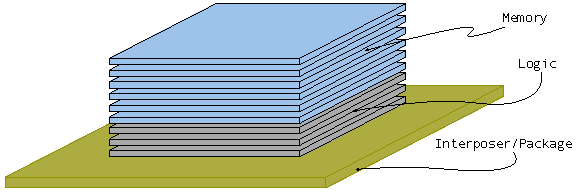
\includegraphics[width=1\textwidth]{DieStack}
  \captionsetup{justification=centering, skip=5pt}
  \caption{Different Die types stacked and mounted on an interposer/package substrate}
  \label{fig:Die Stack}
\end{subfigure}%

\bigskip

\begin{subfigure}{.8\textwidth}
  \centering
  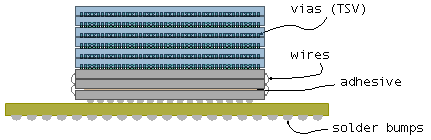
\includegraphics[width=1\textwidth]{DieStackConnections}
  \captionsetup{justification=centering, skip=5pt}
  \caption{Connection Types}
  \label{fig:Die Stack Connection Types}
\end{subfigure}
\captionsetup{justification=centering, skip=12pt}
\caption[3DIC Stack of Die]{3DIC Stack of Die}
\label{fig:3DIC Die}
\end{figure}

\subsection{Pros and Cons}
\label{sec:3dic benefits}

Taking advantage of \acp{3dic} means stacking die on top of one another and making connections directly between the die. These connections can be in the form of wire made at the edges of the die or using vias buried in the die itself.


Below is a summary the benefits of \acp{3dic} :
\begin{outline}
  \1 Reduced Power
    \2 Mainly from not having to drive external outputs and receiving external inputs
  \1 Increased Connectivity
    \2 Maintaining very wide buses through the \ac{soc} increases bandwidth
  \1 Ability to mix heterogeneous technology
    \2 Mixed Analog/Digital
    \2 Mixing memory technology and logic technology
  \1 Increased density and mitigation against the slowing of Moore's Law
    \2 Using the vertical domain to increase perceived transistor per square millimeter
  \1 Potentially lower costs by combining simpler die rather than building a large die
    \2 Yield benefits from combining higher yield die
  \1 Possibility of novel architectures \cite{Kim2016}
\end{outline}

Some disadvantages of \acp{3dic} are:
\begin{outline}
  \1 Reliability
  \1 Cost
    \2 Being a relatively new technology, it is still expensive 
    \2 \ac{tsv} technology is still unreliable
\end{outline}

There is still some reluctance to fully embrace \acp{3dic} but undoubtedly the various barriers will be broken down.
\iffalse
The ability to mix technology targeted toward \ac{dram} with \acs{cmos} is something of which this work takes advantage.
\fi

In \cite{itrs2015_interconn} there are four definitions of \ac{3dic} interconnects:

\begin{outline}
%\section{3D-Wafer level package \cite{itrs2015_interconn}}
%\label{sec:3D-Wafer level package}

  \1 3D-Wafer level package \cite{itrs2015_interconn}
    \2 In this case, different die are stacked and then connected using traditional bond bumps and/or bond wires at the periphery of the chips.
    \2 This technique provides better transistor density compared to traditional 2D-IC with improvements in interconnect density.

%\section{3D-Stacked SoC\ac{soc} \cite{itrs2015_interconn}}
%\label{sec:3D-Stacked \ac{soc}}
  \1 3D-Stacked \ac{soc} \cite{itrs2015_interconn}
    \2 In this case, different die are stacked and then connected using \acp{tsv}. The \acp{tsv} connect the dies to intermediate metal layers known as global metal layers. This allows the individual die to maintain a high level of functionality and thus is similar to connecting functional building blocks, meaning the individual die are likely to be significant functional pieces of \ac{ip}.
    \2 Using \acp{tsv} provides a medium level of interconnect

%\section{3D-Stack \ac{ic} \cite{itrs2015_interconn}}
%\label{sec:3D-Stack \ac{ic}}
  \1 3D-Stack \ac{ic} \cite{itrs2015_interconn}
    \2 In this case, different die are stacked and then connected using \acp{tsv}. The \acp{tsv} connect the dies to intermediate higher metal layers known as global metal layers. This infers the individual dies are not large functioning pieces of \ac{ip}.
    \2 Using \acp{tsv} provides a high level of interconnect

%\section{3D-Integrated Circuit \cite{itrs2015_interconn}}
%\label{sec:3D-Integrated Circuit}
  \1 3D-Integrated Circuit \cite{itrs2015_interconn}
    \2 In this case there are not multiple dies. Instead, the additional silicon layers are deposited on top of each other with the final \ac{3dic} device having multiple layers of transistors
    \2 Local metal layers are used, which along with \acp{tsv} provides a very high level of interconnect
\end{outline}

A die stack with \acp{tsv} can be seen in \fref{fig:tsv}.

\begin{figure}[h]
% the [] contains position info e.g. [!t] means here
\centering
\captionsetup{justification=centering}
\captionsetup{width=.9\linewidth}
\centerline{
\mbox{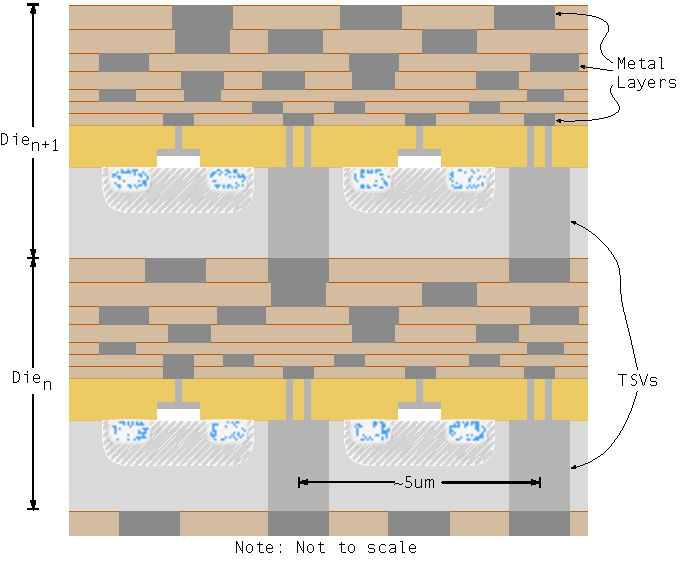
\includegraphics[width=4.5in]{TSVs.pdf}}
}
\caption{Die Stack profile \cite{itrs2015_interconn} with \acp{tsv}}
\label{fig:tsv}
\end{figure}

\subsection{Construction}
\label{sec:3dic construction}

There are other definitions on how the dies are bonded together:
\begin{outline}
  \1 Wafer-to-Wafer
    \2 Current \ac{esd} mitigation allows implementation of unbuffered \ac{io} signals
    \2 Potential low yield because of lack of knowledge regarding \ac{kgd}
  \1 Die-to-Wafer
    \2 Will need additional \ac{esd} mitigation support
    \2 Higher yield because of \ac{kgd}
  \1 Die-to-Die
    \2 Will need additional \ac{esd} mitigation support
    \2 Higher yield because of \ac{kgd}
\end{outline}

This work is targeting \ac{3dic} technology that supports 3D-Stacked \ac{soc} or 3D-Stack \ac{ic} with high levels of interconnect.
To avoid using large \ac{io} buffers for the \ac{tsv} interconnect, this work assumes that the \ac{3dic} technology supports unbuffered interconnects which would suggest wafer-to-wafer bonding.
\iffalse because of the existing \ac{esd} mitigation during wafer handling although it is anticipated that improved \ac{esd} mitigation will be introduced in future manufacturing steps. \fi

\subsection{Design Guidelines}
\label{sec:3dic Design Guidelines}

The technology roadmap in \cite{itrs2015_interconn} and the information in \cite{patti2014} suggest \SI{5}{\micro\meter} pitch \acp{tsv} is a reasonable design goal. 
The dimensions of these \acp{tsv} are of the same order of magnitude as high-level metal layers in a typical 28nm technology node so they are considered to have similar characteristics.
Also, at an operating frequency of \SI[per-mode=symbol]{500}{\mega \hertz}, these \acp{tsv} are not considered to be transmission lines so no additional provisions are needed to route signals between die other than those imposed by the higher metal layers.
However, to provide opportunities for future signal integrity analysis and improvements, this work assumes the \acp{tsv} are arranged in a signal-ground-signal array providing a one-to-one ratio of signal to power/ground \acp{tsv}.
So when accounting for area associated with \acp{tsv}, the number of signal \acp{tsv} is doubled.

As a large amount of \acp{tsv} are employed, \ac{tsv} energy cannot be ignored.
Most of the energy dissipated in the \acp{tsv} is associated with the charging and discharging of the capacitance. 
For \acp{tsv} with \SI{2}{\micro\meter} radius on a \SI{5}{\micro\meter} pitch, \cite{Bamberg2017} suggests an average capacitance of \SI{4.2}{\femto\farad} \footnote{\cite{patti2014} suggests a lower capacitance}.

Assuming a supply voltage of \SI{1.0}{\volt}, the power associated with a \ac{tsv} is shown in \eqref{eq:Energy in a TSV}.
\vspace{-2mm}
\begin{alignat}{2} 
\label{eq:Energy in a TSV}
\text{Energy to charge a \ac{tsv},\hspace{4mm}} E_{tsv} &= \frac{1}{2} \cdot C_{tsv} \cdot V^2  = \frac{1}{2} \cdot \num{4.2e-15} \cdot 1.0 = \SI[per-mode=symbol]{2.1}{\femto \joule} \nonumber \\
\text{Power per \ac{tsv},\hspace{4mm} } P_{tsv} &= E_{tsv} \cdot \text{bit rate} \nonumber \\
\text{normalizing to a clock of \SI{1.0}{\giga\hertz}} & \nonumber \\
\text{Power per \ac{tsv} per \si{\hertz} } &= \SI[per-mode=symbol]{2.1}{\micro \watt \per \giga \bit\per\second \per \ac{tsv}}
\end{alignat}

The \ac{tsv} design guidelines used by this work are summarized in Table \ref{tab:TSV Design Characteristics}.
%Therefore, this work assumes \acp{tsv} with a \SI{5}{\micro\meter} pitch and a power dissipation of \SI[per-mode=symbol]{2.1}{\micro \watt \per \giga \bit\per\second \per \ac{tsv}}.

\begin{table}[h]
  \captionsetup{justification=centering, skip=3pt}
  \caption{TSV design characteristics}
  %\vspace{3pt}
  \label{tab:TSV Design Characteristics}
  \centering
    \begin{adjustbox}{width=0.6\textwidth}
      \begin{tabular}{|c|c|c|c|}\hline
              \multicolumn{2}{|c|}{Dimensions}      &  \multirow{2}{*}{Capacitance}     &  \multirow{2}{*}{Power}                                                                            \\\cline{1-2}
                Pitch        &    Radius           &                                   &                                                                                                    \\\hline
        \SI{5}{\micro\meter} &\SI{2}{\micro\meter} &\SI{4.2}{\femto\farad}             &\SI[per-mode=symbol]{2.1}{\micro \watt \per \giga \bit\per\second \per \ac{tsv}} \cite{Bamberg2017} \\\hline
      \end{tabular}
    \end{adjustbox}
    %\vspace{3pt}
\end{table}







%% Lee
%% In dissertation, change 
%    section* to chapter 
%    subsection* to section
%    subsubsection* to subsection

% >>>>>>>>>>>>>>>>>>>>>>>>>>>>>>>>>>>>>>>>>>>>>>>>>>>>>>>>>>>>>>>>>>>>>>>>>>>>> DRAM Customizable <<<<<<<<<>>>>>>>>>>>>>>>>>>>>>>>>>>>>>>>>>>>>>>>>>>>>>>>>>><<<<<<<<<<<<<
\chapter{DRAM Overview and Customizations}
\label{sec:DRAM Customizations}

There are two types of memory employed in \acp{asic} and \acp{asip}, \acf{sram} and \acf{dram}.
Both of these technologies have a similar top level block diagram which contains an array of storage elements, a means to address into a particular row of memory cells and a means to read and write a column of those cells.
A basic block diagram is shown in figure \ref{fig:MemoryBlockDiagram}.
\begin{figure}[!t]
% the [] contains position info e.g. [!t] means here
\centering
\captionsetup{justification=centering}
\centerline{
\mbox{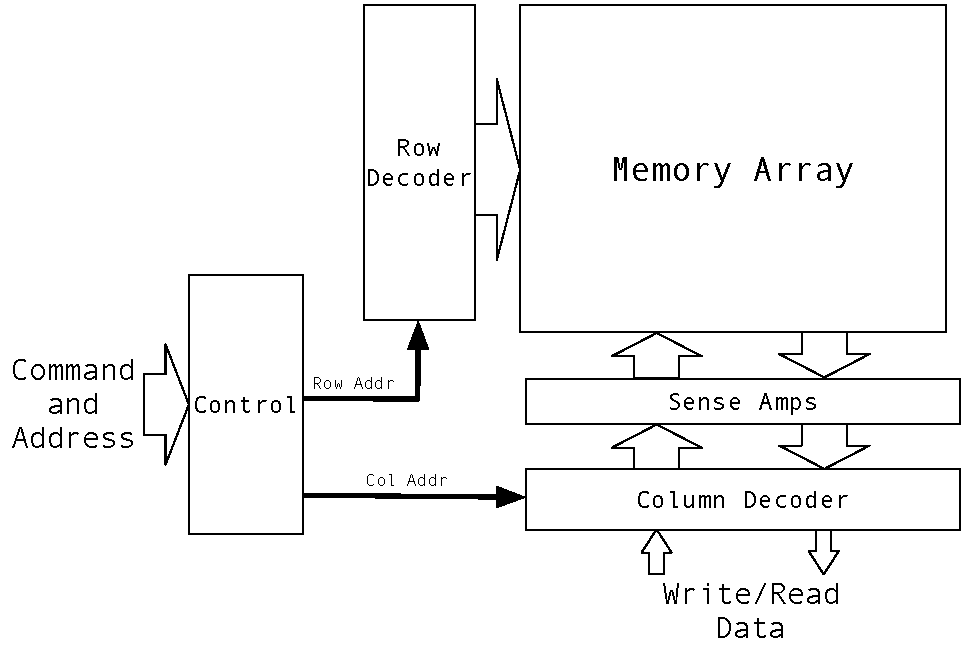
\includegraphics[width=.8\linewidth]{BasicMemoryBlockDiagram}}
}
\caption{Typical Memory Block Diagram \cite{Jacob:2007:MSC:1543376}}
\label{fig:MemoryBlockDiagram}
\end{figure}


\begin{figure}
\centering
\begin{subfigure}{.45\textwidth}
  \centering
  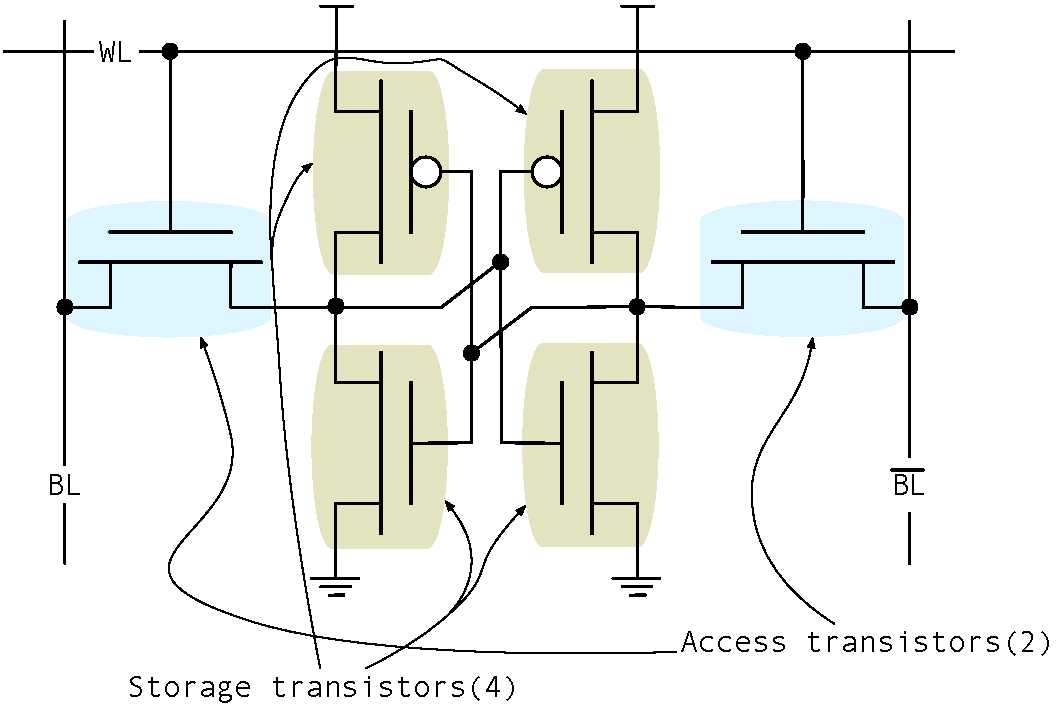
\includegraphics[scale=0.4]{SRAM_Cell}
  \captionsetup{justification=centering, skip=5pt}
  \vspace{-6pt}
  \caption{SRAM Storage Cell \cite{Jacob:2007:MSC:1543376}}
  \label{fig:SRAM Cell}
\end{subfigure}%
\begin{subfigure}{.45\textwidth}
  \centering
  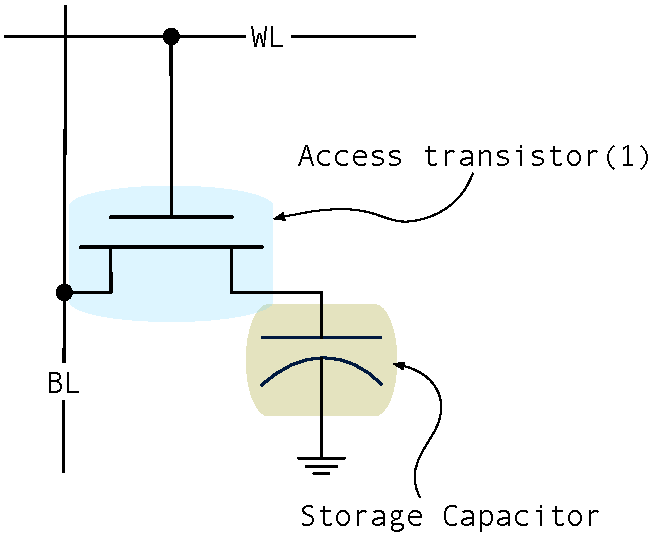
\includegraphics[scale=0.4]{DRAM_Cell}
  \captionsetup{justification=centering, skip=5pt}
  %\vspace{36pt}
  \vspace{20pt}
  \caption{DRAM Storage Cell \cite{Jacob:2007:MSC:1543376}}
  \label{fig:DRAM Cell}
\end{subfigure}
\captionsetup{justification=centering, skip=12pt}
\caption{RAM Storage Cell Types}
\label{fig:Memory Storage Cells}
\end{figure}

The major difference between the \ac{sram} cell and \ac{dram} cell is the number of elements it takes to implement. 
The \ac{sram} cell takes six transistors and the \ac{dram} cell takes one transistor and one capacitor.
The size of the \ac{dram} cell means \ac{dram} arrays provide five to six times more storage density when compared to a similar sized \ac{sram} array.

The major disadvantage is the capacitor cannot hold a indefinitely because the leakage currents in \acp{ic} cause the charge to leak away. 
If kept unchecked, the stored value will dissipate and it is this behavior that makes accessing a \ac{dram} array more complicated than a similar \ac{sram} array.

\section{Accessing \ac{dram} and \ac{sram}}
\label{Accessing DRAM and SRAM}

Accessing a typical \ac{sram} involves providing an address and either reading or writing the contents of that location. 
The read or write often completes in one or two clock cycles depending on whether the \ac{sram} employs internal registers which are used run the \ac{sram} with a faster clock.

The storage cell inside the \ac{sram} is formed from cross-coupled transisters (see figure \ref{fig:SRAM Cell}) which latch the contents and hold the contents indefnitely or until power is removed from the device.
The storage structure employs six transistors and allows the access logic to be relatively simple and fast but has a relatively low density because of the number of transistors employed.

Accessing a "typical" \ac{dram} is much more involved, it involves opening a page in a bank, reading or writing a portion of the contents of the page then closing the page. 

When an \ac{sram} cell is read, the cross-coupled transistors retain the stored value. 
The reasons behind this added complexity is the memory cell inside the \ac{dram} which is formed from a capacitor (see figure \ref{fig:DRAM Cell}) which holds a charge reflecting a logic zero or one. 
When a page(row) of a \ac{dram} memory array is read by the sense amps (see figure \ref{fig:dramBlockDiagram}), the process of sensing the charge on the capacitor causes the capacitor to discharge and lose its contents. 
To alleviate this problem \iffalse \ac{dram} arrays are formed from a column of storage elements known as a page. \fi when the read occurs, the entire contents of the page are transferred to registers, refered to as "page intermediate store" in figure \ref{fig:dramBlockDiagram}. 
The process of transferring a page to the intermediate store is known as a "page open".
Once this transfer is complete, portions of the open page can be read similar to reading an \ac{sram}. 

\iffalse
The value charged on the capacitors are transferred to the page intermediate store and all further reads and writes are to this intermediate store. 

When a different page is accessed, the contents of the page intermediate store has to be returned to the memory array and the capacitors recharged.
The new page can then be transferred to the intermediate store for accessing.
\fi

\iffalse The issue with \acp{dram} is when a storage cell is read, the capacitor is discharged. In addition, sensing this discharging capacitor takes a long time when compared to the \ac{sram} cell.\fi

The problem is that if another read wants to access data that is not in the page, the page has to be closed and another page opened. 
This involves transferring the previously registered page back to the array to recharge the capacitors in the memory array storage elements. 
The next page can then be opened and transferred to the page intermediate registers.

In practice, the \ac{dram} protocol is separated into "page" commands and "cache" commands. The page commands open and close pages and the cache commands read and write to the page intermediate store.

The process of opening and closing pages is a relatively long time, typically 10-20\SI[per-mode=symbol]{}{\nano\second}. Once a page is open, accessing the intermediate store is much faster.
So if the accesses are somewhat random and different pages are constantly accessed and pages are constantly being opened and closed, the average time to complete reads and writes are very large when compared to \ac{sram}.
To alleviate this issue, the \ac{dram} is formed from more than one array of storage elements, between 8 and 32, known as banks. The idea is that while a page from one bank is being accessed, another banks page can be opened in preparation for a future read (or write).
This access protocol is rather complicated and involves interleaving page commands and cache commands to multiple banks. 
The system memory controller logic must keep track of which pages are open inside the \ac{dram} and for each memory request must determine if a page needs to be closed and another opened before reading (or writing) the intermediate store.
If consequtive accesses are not sequenced carefully, the performance of \ac{dram} can be poor.


\subsection{Access Locality/Reuse and \ac{sram} as a Cache}
\label{Access Locality/Reuse and Cache}

In general purpose computing, the sequence of accesses cannot always be controlled, so \ac{sram} is typically used as the first level of memory with \ac{dram} used as the primary storage. 
Using \ac{sram} as this first level memory is called a cache and acts like a mirror of the \ac{dram} contents.
These caches have been used for decades to isolate the computing system from unpredictable access behavior of the \ac{dram}.
The general idea behind caches is that most data exhibits spatial and temporal locality. This "locality" means that when a computer program uses a piece of data in memory, it is very likely that soon after other data "close" to that data will be used and/or the same data will be reused.
So when a piece of data in memory is accessed, that data and a large block of data in close proximity to the requested data are transferred to the cache. 
The cache is designed to hold multiple of these blocks of data often resulting in tens of \SI[per-mode=symbol]{}{\kilo \byte} of \ac{sram}.
When other memory requests are made, the memory controller checks to see whether the block associated with the requested data is present in the cache.
If the requested data is contained in a block present in the cache, this is considered a "hit" and the data in the cache is used. 
If the requested data's block is not present, this is known as a "miss" and the slower main memory must be accessed. This access results in another "block" of data being transferred to the cache.
If all the blocks in the cache are currently fully employed, one of the blocks must be freed up to make space in the cache for the new block. 
A block is chosen and transferred back to the main memory and the new block is read and transferred to the cache.

To make effective use of the cache, the access behavior of the computer program must exhibit this locality behavior. 
If the cache blocks are large enough and the programs access behavior exhibit locality, then employing \ac{sram} is effective and the slower \ac{dram} access times can be somewhat hidden.

As mentioned in section \ref{sec:overview} much of the \ac{asic} and \ac{asip} \ac{ann} research has focused on taking advantage of the performance and ease of use of \ac{sram}. 
If the target application means the memory access behavior exhibits some locality and the \ac{sram} cache can be made large enough to avoid high levels of cache misses, then this use of \ac{sram} can be effective.

But this works target application is such that the access behavior exhibits no or little locality (reuse) and block transfers between the cache and main memory would be constantly occuring.
Under these circustances, \textbf{\textcolor{black}{\ac{dram} bandwidth will be the bottleneck}}.

This work focuses on using \ac{dram} as the primary storage and managing the accesses to ensure the \ac{dram} is used effectively. 
With the increased bandwidth achieved from the additional \ac{dram} customizations discussed in section \ref{sec:Very-Wide Bus} and \ref{sec:Write Mask}, this work demonstrates \ac{dram} bandwidths 10X faster than what is available with 2 or 2.5D solutions.

This high level of \ac{dram} bandwidth provides this work the ability to process multiple disparate \acp{ann} at or near real-time whilst being \textbf{\textcolor{black}{10-100X faster than state-of-the-art solutions}}.


\section{DRAM Customizations}

In a typical \ac{dram}, a bank may contain of the order of a few thousand pages and a page may contain of the order of a few thousand bits.
Once the page is open, the user accesses a portion of the requested page over a bus. With PCB based DRAMs the bus might vary from four to 16 bits wide, but with 3D DRAMs, such as HBM the bus might be up to 128 bits wide.
An \ac{asic}, \ac{asip} or \ac{gpu} implementation may combine multiple devices to generate bus widths of the order of \SI[per-mode=symbol]{1}{\kilo \bit} wide. 
When using 2.5D technology and \ac{hbm} with their Pascal\texttrademark \ac{gpu} accelerator device, NVidia\textregistered ~achieve a raw \ac{dram} bandwidth approaching \SI[per-mode=symbol]{6}{\tera \bit \per \second} \cite{Nvidia_p100_summary_datasheet}\footnote{datasheet also shows a \ac{tdp} of \SI[per-mode=symbol]{300}{\watt}}.
However, experience has shown \cite{farabet2011neuflow} \cite{tensorflow2015-whitepaper} that usable bandwidth will likely be much lower.
Regardless, this existing technology does not achieve the required bandwidth \eqref{eq:maximumBandwidth}.


%Considering systems will want to perform multiple \ac{dnn}s simultaneously suggests that these edge systems will require usable memory bandwidth of the order of 10s of \SI[per-mode=symbol]{}{\tera \bit \per \second} \eqref{eq:maximumBandwidth}.

To achieve increased \ac{dram} bandwidth this work is proposing two changes to the Tezzaron\textregistered \ac{diram4} \cite{tezzaron:diram4} \ac{3d} \ac{dram}. 
The most significant customization is to widen the databuses to generate more raw bandwidth. This is discussed further in section \ref{sec:Very-Wide Bus}.

With the customizations discussed in sections \ref{sec:Very-Wide Bus} and \ref{sec:Write Mask}, this work demonstrates \ac{dram} bandwidths >10X faster than what is available with 2 or 2.5D solutions.

\subsection{Customization One: Very-Wide Bus}
\label{sec:Very-Wide Bus}

Figure \ref{fig:dramBlockDiagram} shows a block diagram of a typical DRAM.

\begin{figure}[!t]
% the [] contains position info e.g. [!t] means here
\centering
\captionsetup{justification=centering}
\centerline{
\mbox{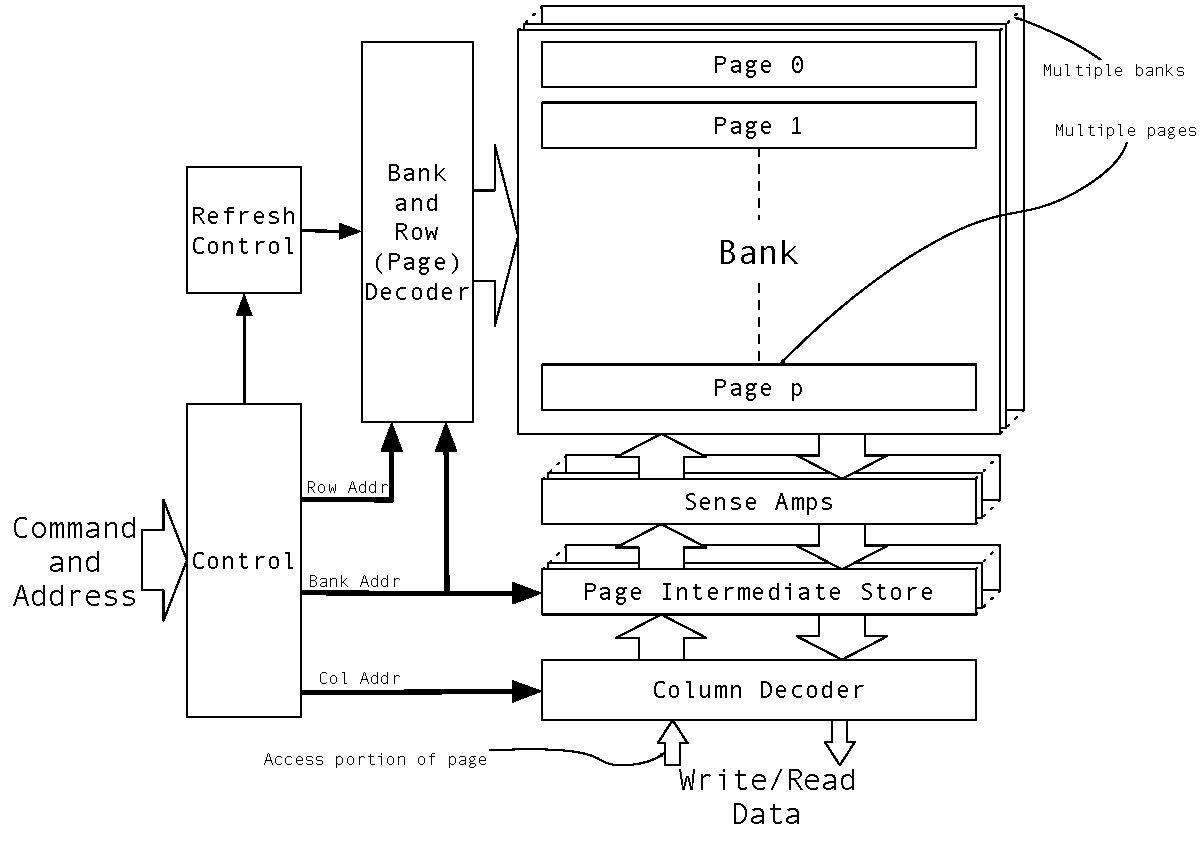
\includegraphics[width=.75\linewidth]{DRAMBlockDiagram}}
}
\caption{Typical DRAM Block Diagram}
\label{fig:dramBlockDiagram}
\end{figure}

This work achieves the increase in bandwidth by proposing that the DRAM expose more of its currently open page.

Without the limitations of having to transfer data beyond the chip stack, this work suggests exposing a larger portion of the page over a very wide bus. By staying within the 3D footprint, this bus can be implemented using fine pitch through-silicon-vias.
(see figure \ref{fig:dramBusChange}).

\begin{figure}[!t]
% the [] contains position info e.g. [!t] means here
\centering
\captionsetup{justification=centering}
\captionsetup{width=.75\linewidth}
\centerline{
\mbox{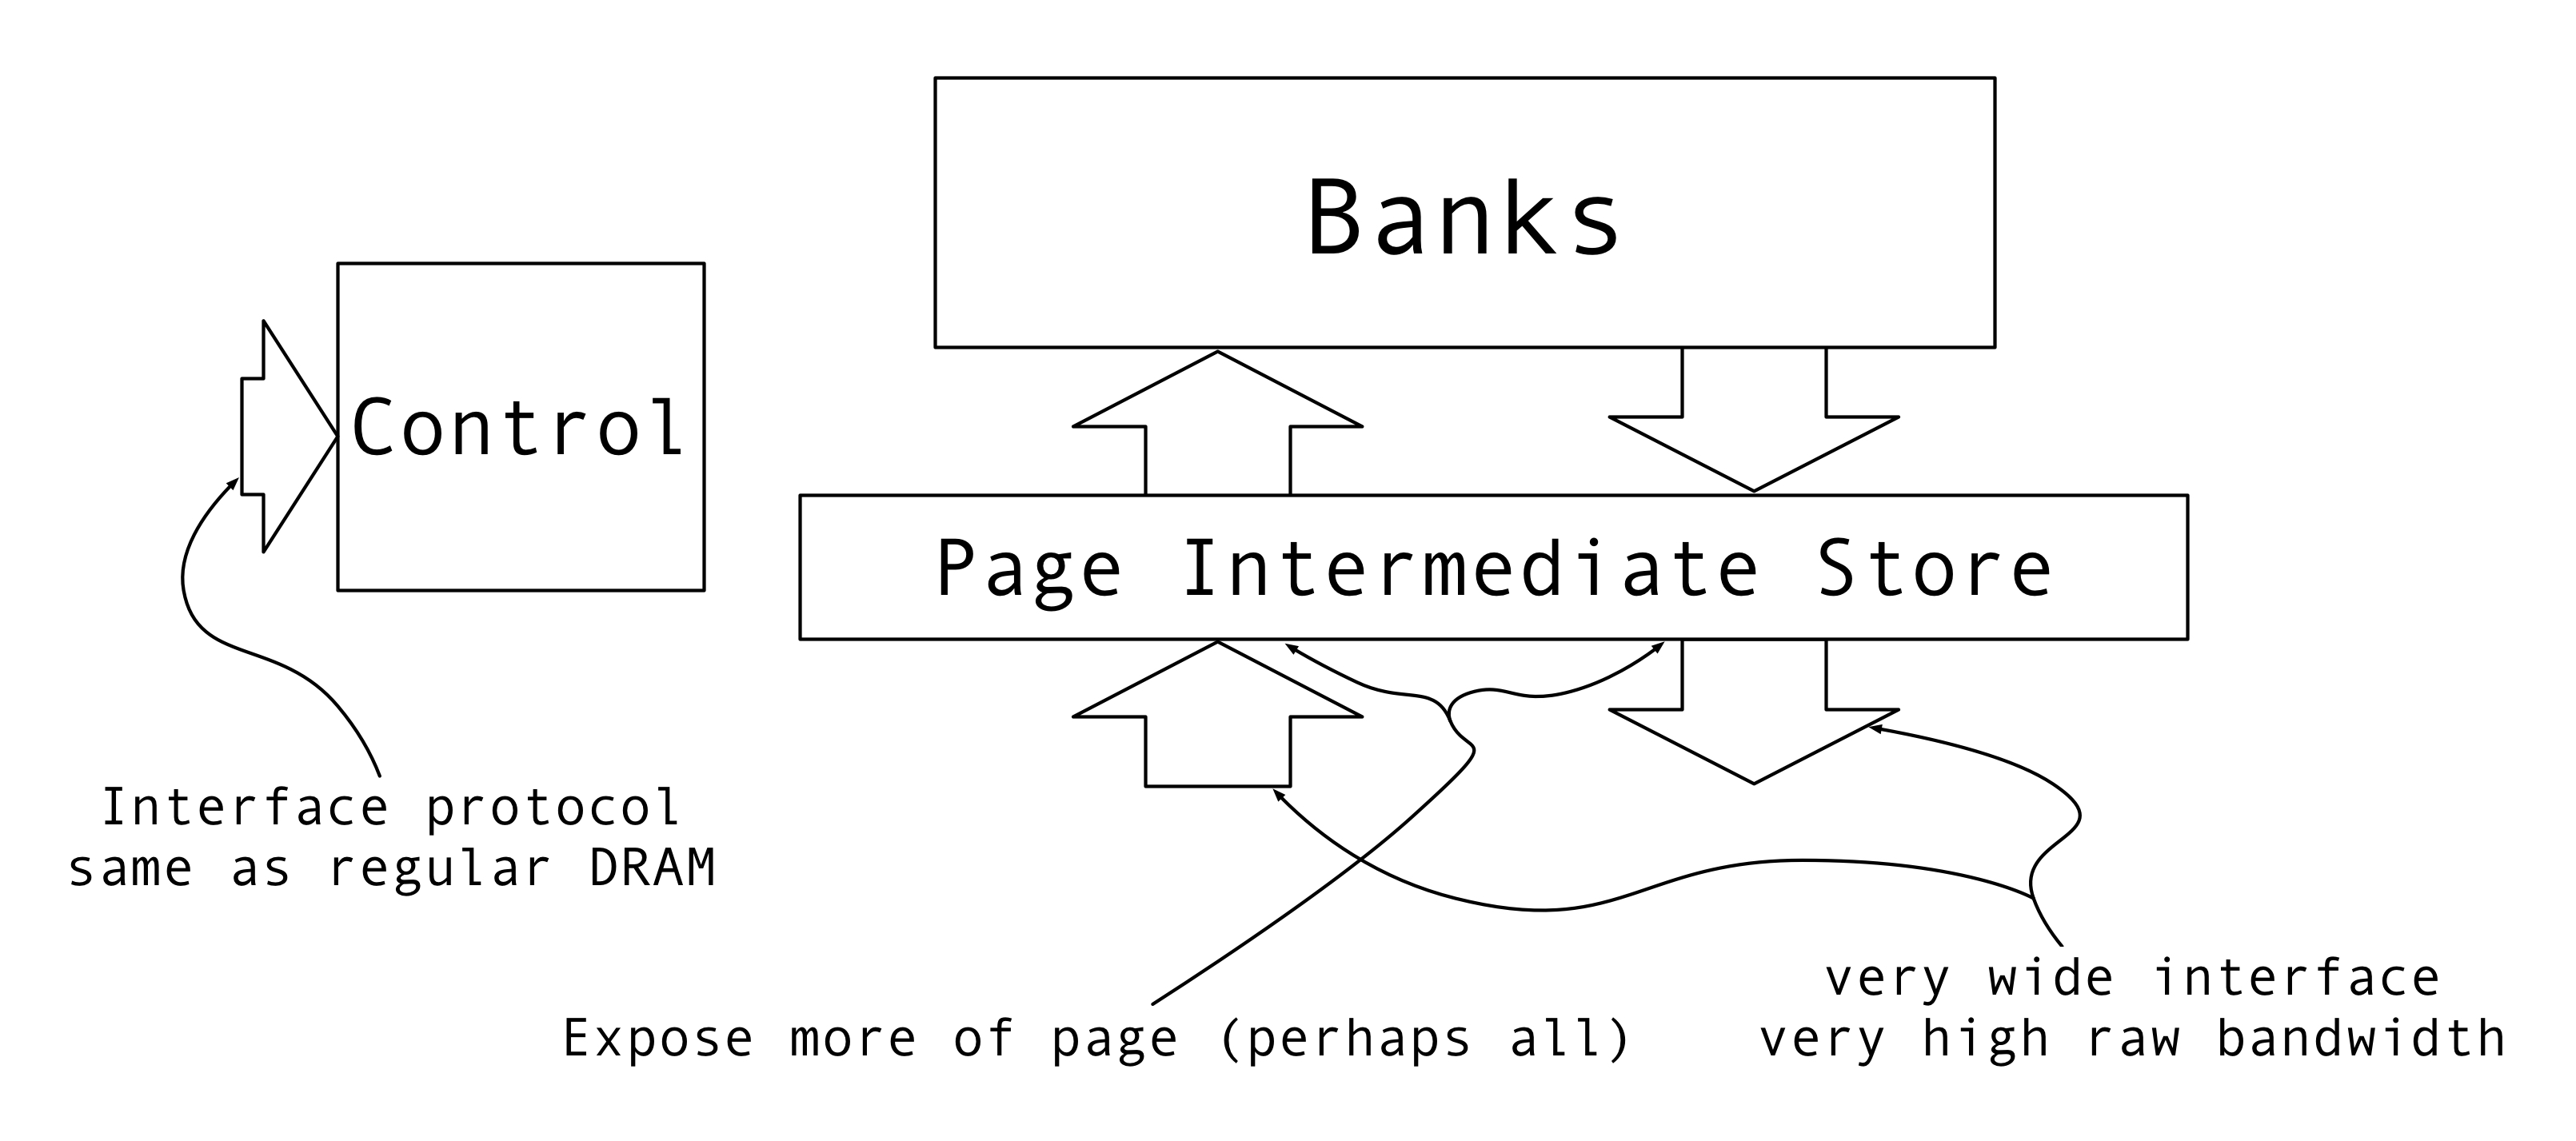
\includegraphics[width=.65\linewidth]{DRAMBusChange}}
}
\caption{Exposing more of the DRAM page}
\label{fig:dramBusChange}
\end{figure}

This work assumes the \ac{dram} interface protocol uses \ac{ddr} with a bus width of 2048. Given the \ac{diram4} employs a burst of two for read and write cycles, an entire \ac{diram4} page of 4096-bits is accessed during each read or write. 

\subsection{Customization Two: Write Mask}
\label{sec:Write Mask}
When processing an ANN, to compute the activation of an individual AN involves reading the pre-synaptic AN activations and the weights of the connections between the pre-synaptic ANs and the AN being processed. The activation of the processed AN is written back to memory. The ratio of reads to writes is high, 100s or 1000s to one. Therefore, the system often needs to write a portion of the page back to memory. To avoid a read/modify/write, a customization to the DRAM is the addition of a write data mask to the DRAM write path.

This work assumes single precision floating point for \ac{ann} weights and activation, so a mask bit will be provided on a word basis or every 32-bits.


%% Lee
%% In dissertation, change section* to chapter and subsection* to section

\chapter{State of the art}
%\section{State of the art}
\label{sec:State of the art}

For the most part, large scale \acp{ann} have been implemented using \acp{gpu}.
In some cases, such as \acp{cnn}, these \acp{gpu} are quite effective when the \ac{ann} parameters can be reused in the \acp{gpu} processor local \ac{sram}.

Much of the \ac{asic} and \ac{asip} research has focused on \acp{cnn} such as \cite{chen201614}\cite{farabet2011neuflow}, 
In some cases, implementations have focused on solving specific processing "hot-spots"\ac{ann} \cite{chen201614}.
%% Dissertation
%% convnets use shared parameters that 
%% a) help with translation invariance
%% b) reduce parameter space
%% \acp{cnn} are not always used in face recognition \cite{Taigman_2014_CVPR}
Almost all \ac{asic} and \ac{asip} solutions employ arrays of \acp{pe} each with local processing capability and local memory.
For most of these, the size of the \ac{ann} supported is limited by the size of the local memory or they are limited to \acp{ann} that have reuse opportunities such as \ac{cnn} or have high batch processing opportunities.
In some cases \iffalse, as seen in \fref{fig:Example state-of-the-art die}\fi the area consumed for local memory can exceed 65\% of the 
processing element die \cite{kim2016neurocube}\cite{chen2014diannao}.

Those that employ external \ac{dram}, such as \ac{tpu} \cite{tensorflow2015-whitepaper}, NnSP{\cite{esmaeilzadeh2005nnsp} and NeuroCube\cite{kim2016neurocube} still 
load weights and \ac{an} states to local \ac{sram} prior to processing although \ac{tpu} assumes all required parameters can be stored in its very large local \ac{sram}.
Others, such as DianNao \cite{chen2016diannao} are moving away from external \ac{dram} toward \ac{edram} thereby acknowledging you need both capacity and \ac{dram} bandwidth. 
But \ac{edram} still has capacity and technology availability issues.

In the case of NnSP{\cite{esmaeilzadeh2005nnsp}, the paper discusses caching data to bridge the speed gap between external memory and the \ac{pe} 
but does not provide details on how to ensure data locality when reading a \ac{dram} cacheline and how to minimize the impact of \ac{dram} protocol.
%% dissertion - mention overlapping kernels etc. ????
%%NnSP recognizes the need to stream from SDRAM but does not address the significant issues associated with
%%data structures in \ac{dram} to facilitate streaming and minimize the access protocol limitations of \ac{dram}.

NnSP does not provide any detail regarding network size and supported types.

Neuflow\cite{farabet2011neuflow} is limited to \acp{cnn} and the external memory is \ac{qdr} \ac{sram} 
and thus will be limited by the network size.

NeuroCube uses a 3D stack along with HMC \ac{3ddram} and data is transferred from the \ac{dram} to the \acp{pe} via a \ac{noc}.
The combination of limited HMC interface bandwidth and the \ac{noc} limits the processing performance for anything other than \acp{cnn}.
%%NeuroCube appears to transfer operands as packets so is not a "stream" processor.

Eyeriss\cite{chen201614} focuses on \acp{cnn} and specifically on the convolution "hot-spots". It does not support the pooling operations although these can
be supported by a local CPU.  However, it does not support the memory intensive fully-connected classifier layers or non weight shared locally-connected layers.
Eyeriss can not be effectively applied to locally-connected type \acp{ann} such as Deepface \cite{Taigman_2014_CVPR}.

The DianNao family of \acp{asic} \cite{chen2014diannao} \cite{chen2016diannao} originally used external \ac{dram} to store \ac{ann} parameters but still \ac{dma} along with \ac{sram}.
However, the later versions of the \ac{asic} have moved from external \ac{dram} to internal \ac{edram} \cite{chen2016diannao} which is still limited to \SI[per-mode=symbol]{36}{\mega \byte} perhaps recognizing you need \ac{dram} for capacity but need high bandwidth for performance.


The Google \ac{tpu} \cite{tensorflow2015-whitepaper} utilizes a large local \SI[per-mode=symbol]{24}{\mega \byte} \ac{sram} along with a 256x256 systolic array and a \SI[per-mode=symbol]{30}{\giga \byte\per\second} external \ac{dram} interface.
It gains performance by storing parameters within the array and by performing large batch processing.
This Google designed solution acknowledges that it is bandwidth limited when implementing the fully connected \acp{ann}.
It also states that their experience of implementing \acp{ann} in the Google server farms suggests that these fully connected \acp{ann} represent the bulk of their processing requirements.
The simpler \acp{cnn} only represent 5\% of the servers \ac{ann} processing requirements.
It should also be stated that this paper also believes that GPU solutions cannot reach the performance targets even though the GPU community might state otherwise.

%% Dissertation
\iffalse
Unlike the current state-of-the-art, this work focuses on processing data as it read out of the \ac{dram} thus avoiding requiring excessive \ac{sram}.
in the \acp{pe} thus allowing optimum logic assignment to the processing functions.
\fi

\iffalse
The current state-of-the-art does not:
%\vspace{-3mm}
\begin{outline}
  %\itemsep-1.5mm
  \1 currently propose streaming data directly from \ac{3ddram} through the processing functions to avoid the use of large local memory
  \1 propose data structures to support continuous streaming from \ac{dram}
  \1 propose a 3D-stack supporting more than one processing layer
%%  \item provide specific special streaming functions to support a family of \acp{ann}
\end{outline}
%%%
\fi

%% Dissertation
\iffalse
%\vspace{-5mm}
\begin{figure}
\centering
\begin{subfigure}{.45\textwidth}
  \centering
  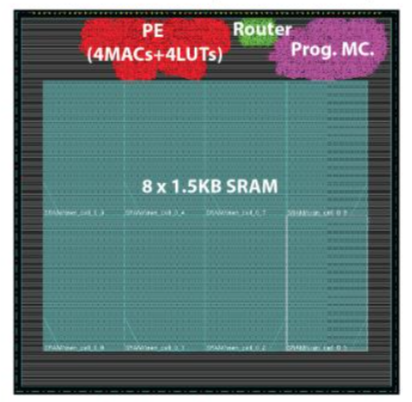
\includegraphics[width=0.8\textwidth]{kim2016neurocube_fig4}
  \captionsetup{justification=centering, skip=6pt}
  \caption{NeuroCube}
  \label{fig:NeuroCubeDie}
\end{subfigure}%
\begin{subfigure}{.45\textwidth}
  \centering
  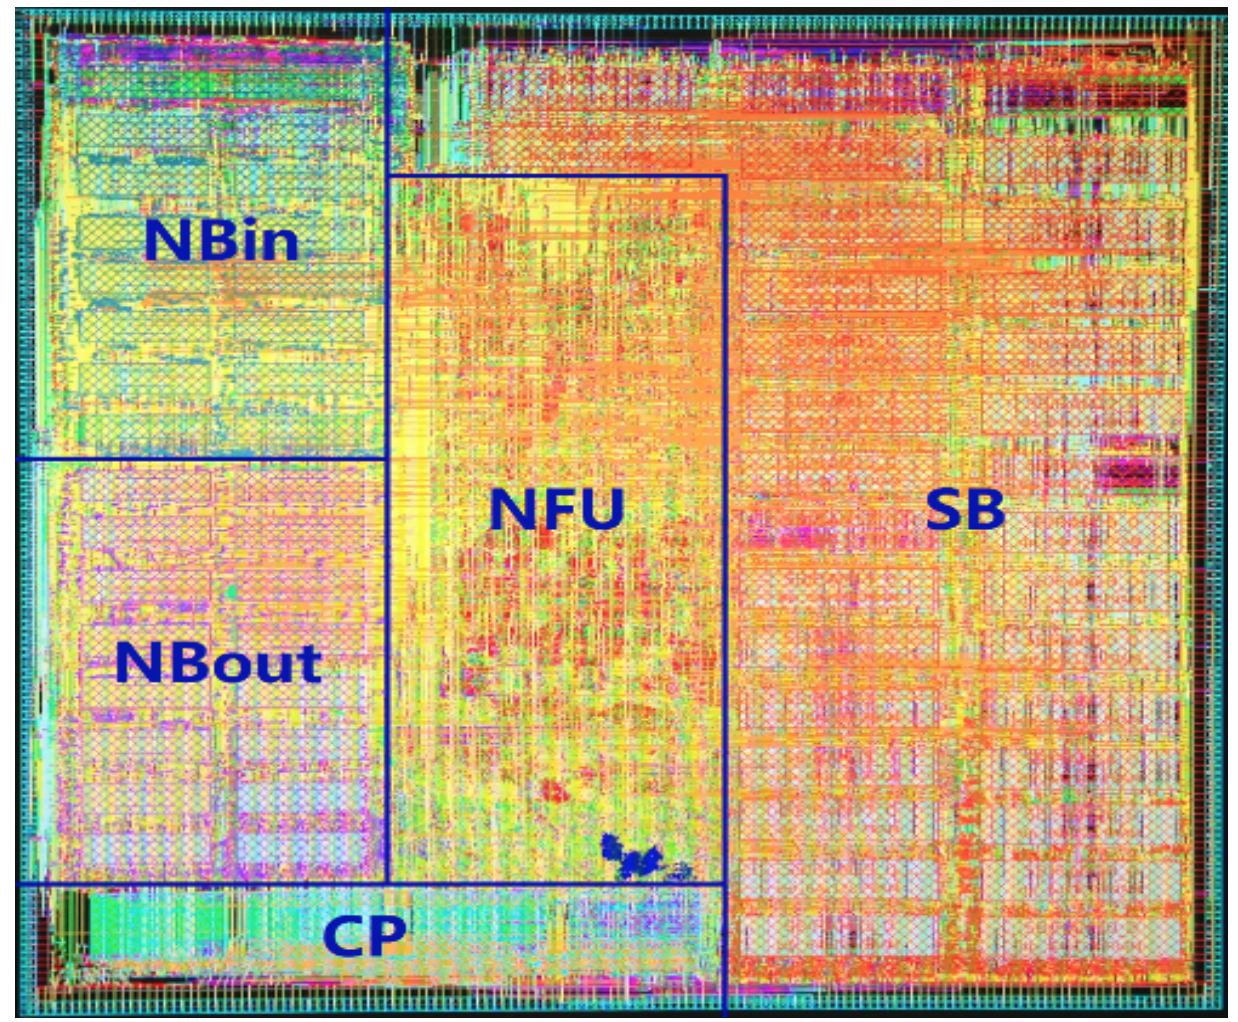
\includegraphics[width=0.8\textwidth]{chen2014diannao_fig15}
  \captionsetup{justification=centering, skip=10pt}
  \caption{Diannao (SB and NBx are \ac{sram})}
  \label{fig:DiannaoDie}
\end{subfigure}
\captionsetup{justification=centering, skip=3pt}
\caption{Example state-of-the-art die}
\label{fig:Example state-of-the-art die}
\end{figure}
%\vspace{-5mm}
\fi


%% Uncomment for dissertation
\iffalse

NeuroCube\cite{kim2016neurocube} is the only solution to explicitly discuss \ac{3d} memory but will be limited by its focus on utilizing local \ac{sram} where our focus is on
providing silicon for processing and not local storage.
Neuflow\cite{farabet2011neuflow} has processing elements that are limited to \acp{cnn}.
NnSP{\cite{esmaeilzadeh2005nnsp} transfers weights and inputs to local \ac{pe} memory prior to processing.
nn-X\cite{gokhale2014240} limits the number format to integer, and although there is some acceptance that similar
results can be obtained compared to floating point, this will likely limit the applcation space. 
nn-X is also limited to performing the convolution operation and \ac{sram} size will limit its capability when performing the classifier stage.

Below is a summary of current technology.

\section[NnSP]{NnSP{\cite{esmaeilzadeh2005nnsp}}}

Uses external \ac{dram} with a cache.
Does not address the main issue of DRAM access limitations and providing data structures.
It simply says "use a cache" but doesnt justify locality issues.

Transfers weights and inputs to local \ac{pe} prior to processing
Similar "Streaming" terminlogy but streams from local memory.
\ac{an} outputs are kept locally and transferred to other \ac{an} via an  \ac{noc}.

No detail on processing element but likely limited to "standard" feedforward \acp{ann}.


%% Note: add \section[<section>]{<section> \cite{}} instead of \section{<section> \cite...}
%% to avoid case mismatch issues when running bibtex
\section[NeuroCube]{NeuroCube{\cite{kim2016neurocube}}}
NeuroCube\cite{kim2016neurocube} transfers data to \ac{pe} prior to processing which can limit classifier size although most
convolution kernels can be supported.
The \ac{sram} on the \ac{pe} is significant (see \fref{fig:NeuroCubeDie}).
NeuroCube uses HMC \ac{3ddram} which has limited bandwidth and this will limit network processing performance.
The NeuroCube implements a processing layer but does not address adding additional layers. 

3D uses HMC
 - limited by HMC bandwidth
 - is serdes a good choice for die-to-die communication (typically used for die to chip/board?)
 - doesnt really discuss adding additional layers

Transfers data to \ac{pe} prior to processing


\section[IMAPCAR]{IMAPCAR \cite{kyo2011imapcar}}
IMAPCAR uses external \ac{sram} so will be limited by network size.
The architecture of IMAPCAR is optimized for processing video.

In general will not scale to \acp{ann} of interest.


\section{NeuFlow \cite{farabet2011neuflow}}
Neuflow\cite{farabet2011neuflow} has processing elements that are "highly optimized" to \acp{cnn}.
Neuflow is designed around external \ac{qdr} memory and does not address the issues associated with supporting large networks.


\section[nn-X]{nn-X \cite{gokhale2014240}}
nn-X\cite{gokhale2014240} limits the number format to integer, and although there is some acceptance that similar
results can be obtained, this will likely limit the applcation space. nn-X is also limited to performing the convolution operation
and \ac{sram} size will limit its capability when performing the classifier stage.
nn-X was implemented in an fpga and does not address \ac{sram} size when scaling to larger networks.


\section[Diannao]{Diannao \cite{chen2014diannao}}
Diannao\cite{chen2014diannao} acknowledges the need for large amounts of storage which will exceed the capability of local memory.
The kernel sizes are limited by \ac{sram} size although it does state kernels can be "broken up".
The \ac{sram} use on the \ac{pe} is significant (see \fref{fig:DiannaoDie}).


\section[Eyeriss]{Eyeriss \cite{chen201614}}
Eyeris\cite{chen201614} focuses on \acp{cnn} and specifically the convolution stage.
Eyeriss ignores the pooling and classifier stages which although not as compute intensive they are memory intensive.
Therefore Eyeriss limits network size and does not implement the network.

\section[TPU]{TPU \cite{jouppi2017datacenter}}
The TPU utilizes an 256x256 array of \num{64e3} processing elements and demonstrates significant (~30X) performance improvements over \acp{gpu} and \acp{cpu}. It does employ DRAM which provides the required storage capacity
but employs SRAM as an intermediate store between the DRAM and the \acp{pe}.
This Google designed solution acknowledges that it is bandwidth limited when implementing the fully connected \acp{ann}.
It also states that their experience of implementing \acp{ann} in the Google server farms suggests that these fully connected \acp{ann} represent the bulk of their processing requirements.
The simpler \acp{cnn} only represent 5\% of the servers \ac{ann} processing requirements.
It should also be stated that this paper also believes that GPU solutions cannot reach the performance targets even though the GPU community might state otherwise.


\fi



%%%%%%%%%%%%%%%%%%%%%%%%%%%%%%%%%%%%%%%%%%%%%%%%%%%%%%%%%%%%%%%%%%%%%%%%%%%%%%%%%%%%%%%%%%%%%%%%%%%%%%%%%%%%%%%%%%%%%%%
%%%%%%%%%%%%%%%%%%%%%%%%%%%%%%%%%%%%%%%%%%%%%%%%%%%%%%%%%%%%%%%%%%%%%%%%%%%%%%%%%%%%%%%%%%%%%%%%%%%%%%%%%%%%%%%%%%%%%%%
%%%%%%%%%%%%%%%%%%%%%%%%%%%%%%%%%%%%%%%%%%%%%%%%%%%%%%%%%%%%%%%%%%%%%%%%%%%%%%%%%%%%%%%%%%%%%%%%%%%%%%%%%%%%%%%%%%%%%%%
%%%%%%%%%%%%%%%%%%%%%%%%%%%%%%%%%%%%%%%%%%%%%%%%%%%%%%%%%%%%%%%%%%%%%%%%%%%%%%%%%%%%%%%%%%%%%%%%%%%%%%%%%%%%%%%%%%%%%%%
%%%%%%%%%%%%%%%%%%%%%%%%%%%%%%%%%%%%%%%%%%%%%%%%%%%%%%%%%%%%%%%%%%%%%%%%%%%%%%%%%%%%%%%%%%%%%%%%%%%%%%%%%%%%%%%%%%%%%%%



%% Lee
%% In dissertation, change section* to chapter and subsection* to section


\chapter{System Overview}
\label{chap-five}
\label{sec:System Overview}
As mentioned in chapter \ref{sec:Introduction} and chapter \ref{Motivation}, this works target application implements mulltiple \acp{ann} each of which have limited opportunities for both weight reuse and batch processing.
These requirements require \ac{dram} to be employed for main storage of \ac{ann} parameters and local \ac{sram} is of limited use.
Under these conditions, the \ac{dram} bandwidth is the system bottleneck.

To meet these requirements, this work proposed employing \acp{3dic} technology along with a customized \ac{3d} \ac{dram} and \ac{asic} technology. 
By physically staying within the \ac{3dic} footprint and taking advantage of high density \acp{tsv} this work is able to maintain a significantly higher bandwidth over 2D or 2.5D \ac{asic} or \ac{asip} solutions.
The objective was to demonstrate that a pure \ac{3dic} system can implement multiple disparate \acp{ann} within reasonable power and area constraints. 

The \ac{3dic} system die stack (figure \ref{fig:3DICStack}) includes the \ac{3d}-\ac{dram} with a system manager below and one or more processing layers below the manager.
\begin{figure}[!t]
% the [] contains position info e.g. [!t] means here
\centering
\captionsetup{justification=centering}
\captionsetup{width=.9\linewidth}
\centerline{
\mbox{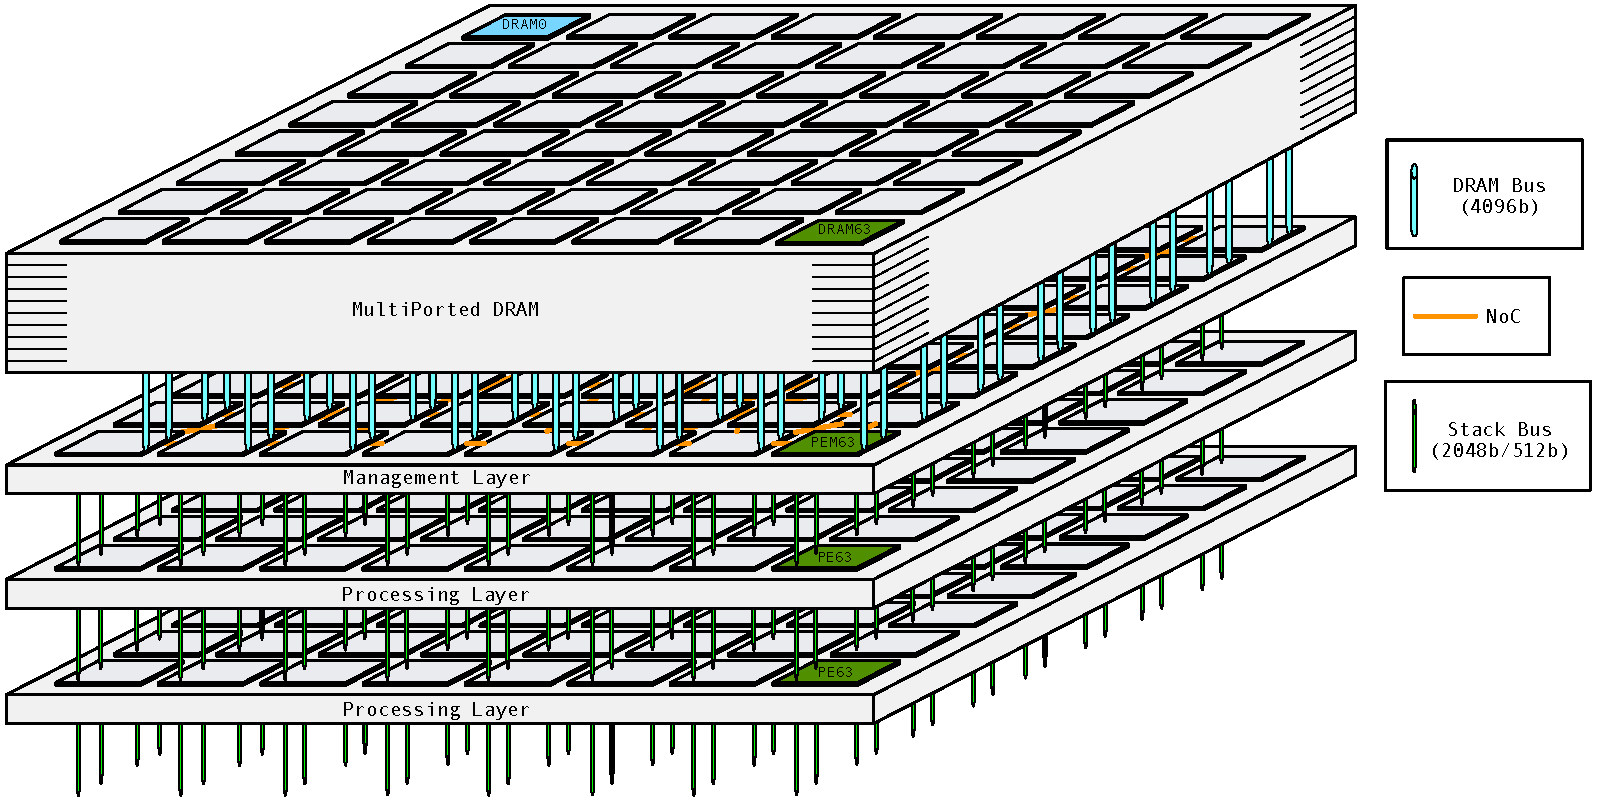
\includegraphics[width=.9\linewidth]{StackDiagram}}
}
\caption{3DIC System Stack}
\label{fig:3DICStack}
\end{figure}

3D-DRAM has recently become available in standards such as \ac{hbm} and \ac{hmc} and proprietary devices such as the DiRAM4 available from Tezzaron. 
These technologies provide high capacity within a small footprint.

In the case of \ac{hbm} and \ac{diram4} \cite{tezzaron:diram4}, the technology can be combined with additional custom layers to provide a system solution.

The question becomes, can a useful system coexist within the same 3D footprint?

This work targeted a baseline system with:
\begin{outline}
  \1 Computations requiring \ac{binary32}
  \1 Tezzaron \acf{diram4} \cite{tezzaron:diram4} for main memory
  \1 28nm \ac{asic} technology
\end{outline}
The work includes customizing the interface to a 3D-\ac{dram}, researching data structures to describe storage of \ac{ann} parameters, designing a memory manager with unique micro-coded instructions and a \ac{pe} layer.  
The targeted 3D-\ac{dram}, the Tezzaron DiRAM4 employs 64 disjoint memories arranged in a physical array.


\section{Sub-System Column}
\label{sec:Sub-System Column}

The overall system is constructed from an array of sub-systems known as a \acf{ssc} which combines the manager logic, \ac{dram} and \ac{pe} logic.
The various steps to process an \ac{ann} are provided in the form of instructions (see section \ref{sec:Instructions}. 
The instructions are downloaded by a host system to instruction memory residing in the manager.
The manager decodes these instructions and based on the instruction contents is responsible for coordinating \ac{ssc} operations and managing the reading and writing of \ac{dram}.
With the processing of an \ac{an}, the manager reads pre-synaptic states and connection weights from the \ac{dram}, provides that data to the \ac{pe} which operates on data and returns any results back to the manager.
There are other instructions that specifically deal with coordination between \ac{ssc} but the main workload is the processing of the \acp{an}.

The \ac{ssc} has been designed for extensibility to allow future modifications to support different number formats, different \ac{pe} configurations and to allow additional features to be implemented without a significant increase in logic area.

The \ac{ssc} is designed to operate on one of the disjoint sub-memories within the \ac{diram4} (see figure \ref{fig:diram4Layout}).
As shown in figure \ref{fig:SSC}, the \ac{ssc} includes the \ac{diram4} sub-memory (referred to as the \ac{ssc} memory), a manager module and a \ac{pe} module.
\begin{figure}
\centering
\begin{subfigure}{.44\textwidth}
  \centering
  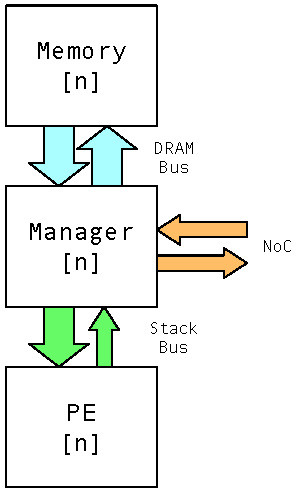
\includegraphics[scale=0.75]{SSC_logical}
  \captionsetup{justification=centering, skip=10pt}
  \vspace{-6pt}
  \caption{Sub-system column logical block diagram}
  \label{fig:Sub-system Column Logical Block Diagram}
\end{subfigure}%
\begin{subfigure}{.54\textwidth}
  \centering
  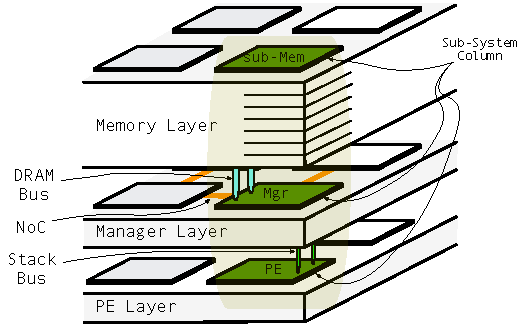
\includegraphics[scale=0.9]{SSC_physical}
  \captionsetup{justification=centering, skip=10pt}
  %\vspace{36pt}
  \vspace{20pt}
  \caption{Sub-system column physical diagram}
  \label{fig:Sub-system Column Physical Diagram}
\end{subfigure}
\captionsetup{justification=centering, skip=12pt}
\caption{\acf{ssc}}
\label{fig:SSC}
\end{figure}

The customizations described in section \ref{sec:Very-Wide Bus} means each \ac{ssc} memory provides the manager with a 2048-bit \ac{ddr} data bus.
The \ac{diram4} has 64 sub-memories so there are 64 \acp{ssc}. The \ac{ssc} has been designed as a standalone unit and does not have a direct knowledge of the other \acp{ssc} in the system.

To process an \ac{ann}, the user must allocate the individual \acp{an} to an \ac{ssc}. Once partitioned, a \acp{ann} pre-synaptic connection weights must be stored in the \ac{ssc} memory associated with the \ac{an}.
The states of the pre-synaptic \acp{an} must also be stored in a dependent \acp{an} allocated \ac{ssc} memory.
Details on where the parameters and \ac{an} states are stored are described in chapter \ref{sec:System Operations}.

The baseline \ac{ssc} is designed with 32 execution lanes each of which can simultaneously process two streams of \ac{binary32} words.
The customized \ac{diram4} provides a 2048-bit cacheline at the system clock rate to the manager. This 2048-bit bus is sub-divided into 64 \ac{binary32} words.
The manager layer reads the 2048-bit cacheline from the \ac{dram}, multiplexes the 64 words onto 32 execution lanes with two words per execution lane and passes the execution lane data to the \ac{pe} layer.
The primary function is to direct a pre-synaptic \ac{an} state and connection weight to the two words in an execution lane where they are multiplied and accumulated by the \ac{pe} layer.

The manager layer has individual stream read memory controllers to allow the individual streams in the execution lanes to operate independently.
In this way, the \ac{an} states and the connection weights can be stored in different configurations depending on the \ac{ann} type and \ac{ann} partitioning.
The 32 execution lanes can be used for processing a group of one to 32 individual \acp{an} or for processing one \ac{an}.

\section{Processing a group of \acp{an}}
\label{sec:Processing a group of ANes}

In the case of group of \acp{an}, all the \acp{an} must be associated with a \ac{roi} or a fully-connected layer.
The pre-synaptic \ac{roi}, or all the \acp{an} in the case of a fully-connected layer, are broadcast to one of the streams of all execution lanes.
The other stream is used for the individual \acp{an} connection weights. 
The \ac{pe} \ac{stop} performs 32 simultaneous \acf{fp} \ac{mac} operations while the data is being streamed from the manager layer to the \ac{pe} layer.
Once all the \ac{an} states and weights have been streamed to the \ac{pe}, the \ac{stop} passes the result of the \ac{mac} to the \ac{pe} \ac{simd} which then applies the activation function.
Typically the \ac{simd} then sends states of the group of \acp{an} back to the manager.

Considering the pre-synaptic \ac{an} states $A_p$ and weights $W_p$ as arrays $\left[A\right]$ and $\left[W\right]$, the state of the \ac{an} is the dot-product of the two arrays followed by the activation function \eqref{eq:AN dot-product function} and how the weights and states are directed to execution lanes are shown in figure \ref{fig:AN group multiplexing}.

%\vspace{-1cm}
\begin{alignat}{2} 
  \label{eq:AN dot-product function}
  \text{\ac{an} State }   &= f\big(\left[W\right] \mathbf{\cdot} \left[A\right]\big)  \\
  \text{where } &\mathbf{W}=\left[w_0, w_1, \dots w_n \right], \quad \mathbf{A}=\left[a_0, a_1, \dots a_n \right] \notag \\
  \text{and } &n \text{ is the pre-synaptic fanin              \notag }
\end{alignat}

\begin{figure}[h]
\centering
\begin{subfigure}{.44\textwidth}
  \centering
  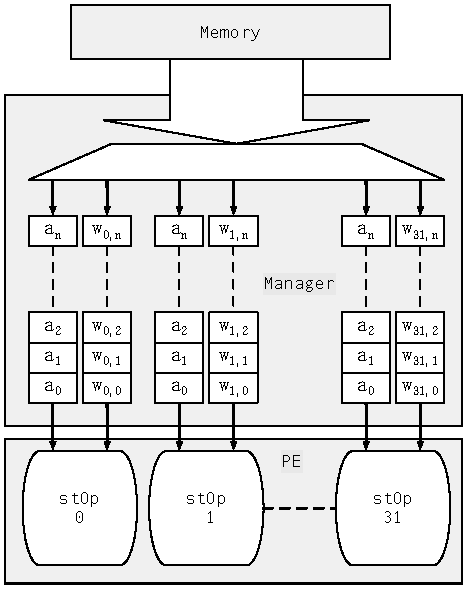
\includegraphics[scale=0.75]{groupANmultiplexing}
  \captionsetup{justification=centering, skip=10pt}
  %\vspace{-6pt}
  \caption{Multiplexing \ac{dram} data for a \ac{an} group} 
  \label{fig:AN group multiplexing}
\end{subfigure}%
\begin{subfigure}{.54\textwidth}
  \centering
  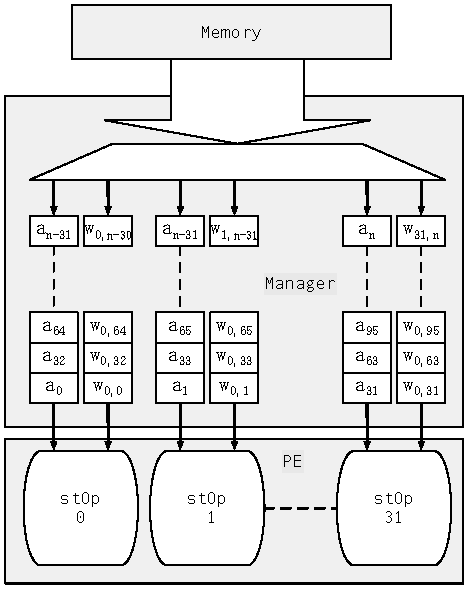
\includegraphics[scale=0.75]{singleANmultiplexing}
  \captionsetup{justification=centering, skip=10pt}
  %\vspace{-6pt}
  \caption{Multiplexing \ac{dram} data for a single \ac{an}} 
  \label{fig:Single AN multiplexing}
\end{subfigure}
\captionsetup{justification=centering, skip=12pt}
\caption{Multiplexing \ac{dram} data to execution lanes}
\label{fig:DRAM data multiplexing}
\end{figure}

\section{Processing a single \ac{an}}
\label{sec:Processing a single of ANes}

In the case of a single \acp{an}, the pre-synaptic \ac{an} states are vectored across one of the streams of all execution lanes.
The connection weights are vectored across the other stream of all the execution lanesall the \acp{an} must be associated with a \ac{roi} or a fully-connected layer.
How the weights and states are directed to execution lanes are shown in figure \ref{fig:Single AN multiplexing}.

An overview of the various blocks and interconnects in the \ac{ssc} are given in section \ref{sec:SSC Blocks} with additional detail provided in chapter \ref{sec:Detailed System Description}.

% ----------------------------------------------------------------------------------------------------
\section{\acf{ssc} Blocks}
\label{sec:SSC Blocks}

\subsection{Customized \ac{dram} : \acf{diram4}}
\label{sec:3ddram}
The \ac{diram4} \cite{tezzaron:diram4} employs multiple memory array layers in conjunction with a control and IO layer.
The memory is formed from 64 disjoint sub-memories each providing upwards of \SI[per-mode=symbol]{1}{\giga\bit} with a total capacity of at least \SI[per-mode=symbol]{64}{\giga\bit}.
Unlike traditional \ac{dram}, the \ac{diram4} has two independent channel which are accessed using \ac{ddr} signalling on the control signals.
Each channel has 32 banks and 4096 pages per bank with \SI[per-mode=symbol]{4096}{\bit\per page}.

The standard \ac{diram4} has a 32-bit read databus and a 32-bit write databus enabling simultaneous read and write. Both read and write databuses employ \ac{ddr} signaling.
The read and write transactions are burst-of-two providing 64bits per read/write. When accessing a \ac{dram}, a read and write are often referred to as a cacheline.
The device is designed to operate at \SI[per-mode=symbol]{1}{\giga\hertz} although this work targeted a \SI[per-mode=symbol]{500}{\mega\hertz} clock frequency.

This work is proposing customizations to the \ac{diram4} which are outlined in chapter \ref{sec:DRAM Customizations}. One of these proposed changes is to widen the read and write databuses to 2048-bits.
Using the same burst-of-two means each read and write will access an entire page. A cacheline becomes 4096-bits.
Another proposed change is the add mask bits to the write databuse to avoid having to perform read/modify/writes when writing back data much smaller than the new large cacheline.

\begin{figure}[!t]
% the [] contains position info e.g. [!t] means here
\centering
\captionsetup{justification=centering}
\captionsetup{width=.9\linewidth}
\centerline{
\mbox{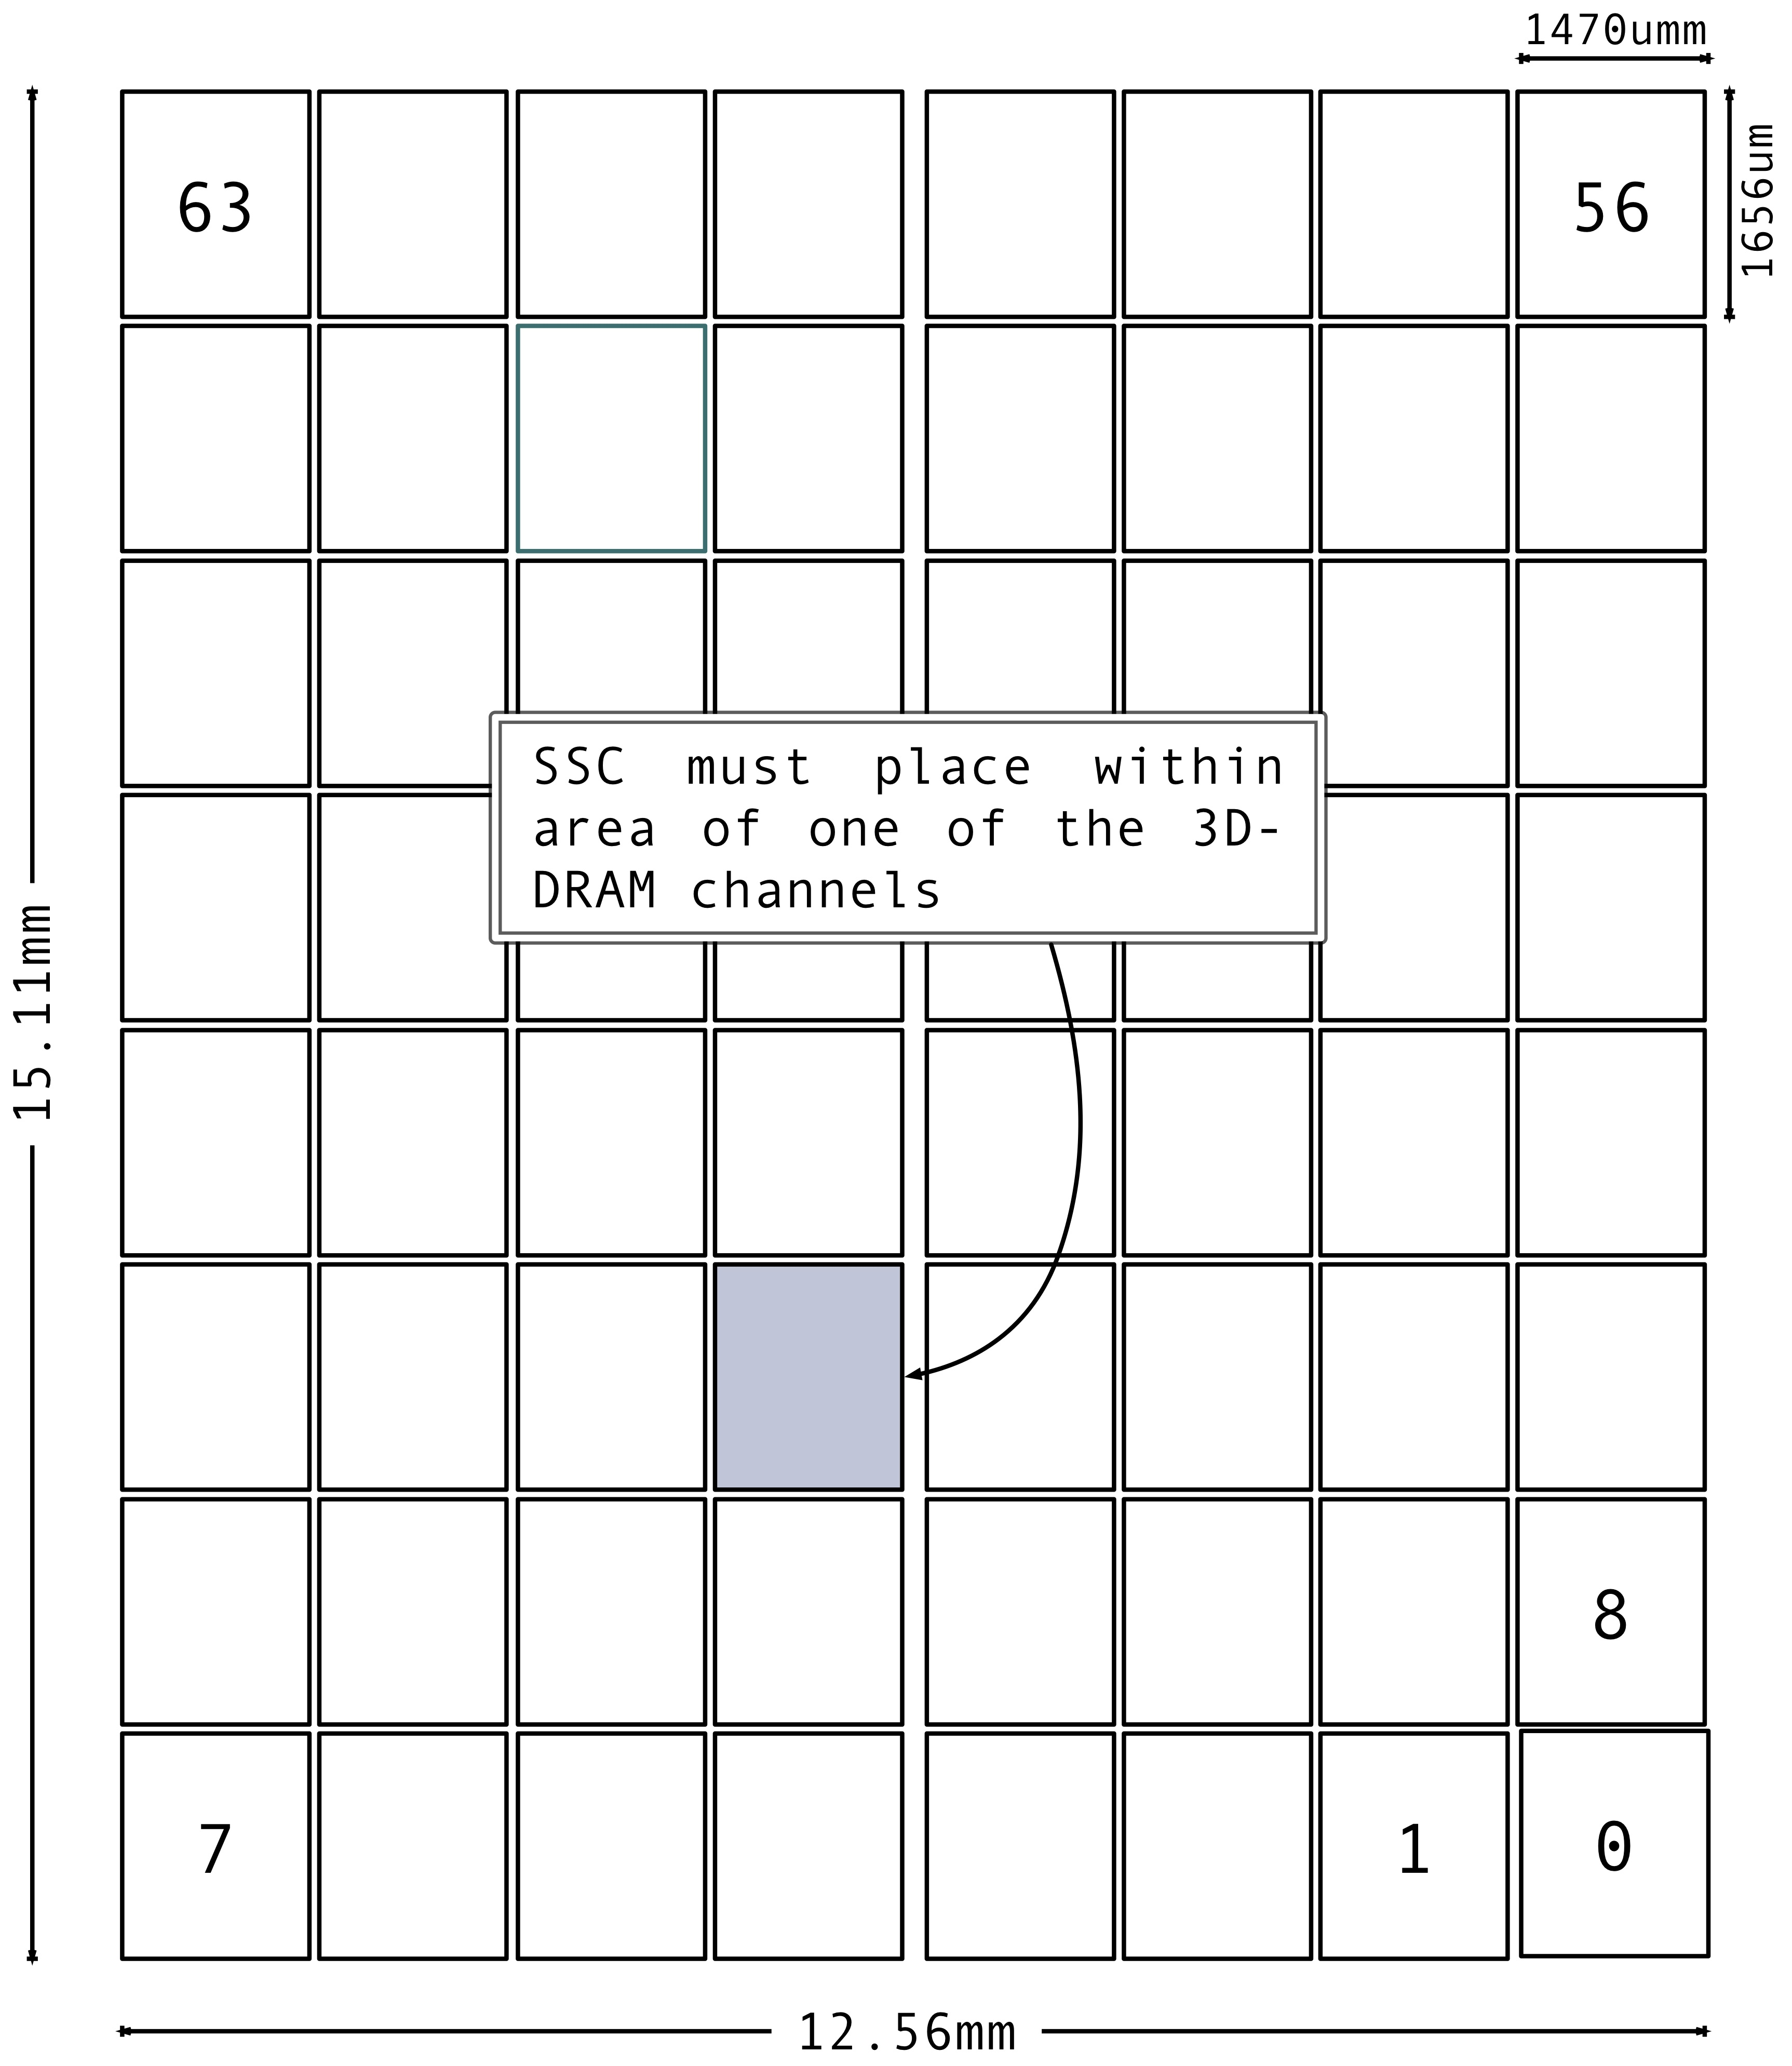
\includegraphics[width=.4\linewidth]{DiRAM4Layout}}
}
\caption{\ac{dram} Physical Interface Layout showing area for \ac{ssc}}
\label{fig:diram4Layout}
\end{figure}


% ----------------------------------------------------------------------------------------------------
\subsection{Layer Interconnect}
\label{sec:Layer Interconnect}

The layers are connected using through-silicon-vias (\ac{tsv}s) which provide high connection density, high bandwidth and low energy.
By ensuring the system stays within the 3D footprint ensures we can take advantage of the area and bandwidth benefits provided by \acp{tsv}.
The high density interconnect provided by \acp{tsv} allows the system to take advantage of the very wide \ac{dram} bus provided by the \ac{dram} customization described in section \ref{sec:Very-Wide Bus}.
The wide interconnect between the manager and \ac{pe} are also implemented using \acp{tsv}.

The interconnect between the manager and \ac{pe} is referred to as the stack bus. The interconnect between the manager and \ac{dram} is referred to as the \ac{dram} bus.

\subsection{Stack Bus}
\label{sec:Stack Bus}

The stack bus is bidirectional with a 36-bit \ac{oob} configuration bus from the manager to the \ac{pe}, a 2048-bit "downstream" data bus from the manager to the \ac{pe} and a 512-bit "upstream" data bus from the \ac{pe} to the manager.

The 36-bit \ac{oob} bus is designed to send configuration packets to configure the \ac{stop} and \ac{simd} blocks inside the \ac{pe}.
The packet primarily contains the \ac{stop} function to be performed on the downstream data and the operation the \ac{simd} is to perform on the result from the \ac{stop}.
It also includes the size of the downstream data stream and an operation idenfication tag.

In teh baselne system, the 2048-bit downstream stack bus is designed to carry 32 execution lanes of data with each execution lane containing two operand buses. 
The two operand buses are designed to carry streams of \ac{binary32} numbers.
This allows the downstream stack bus simultaneously stream 32 execution lanes each with two 32-bit argument streams. 
Typically these streams are the weights and pre-synaptic \ac{an} states to calculate the states of up to 32 \acp{an}. 
The streams can also be configured to calculate the state of a single \ac{an} where the weights and pre-synaptic \ac{an} states for the single \ac{an} are sent in parallel across the downstream stack bus and a reduction operation can be performed in the \ac{pe} by the \ac{stop} and \ac{simd}.

The 512-bit upstream bus is primarily designed to send the results of a downstream operation. Typically this is the states of up to 32 \acp{an}.
The upstream bus is packetized with the result data contained in the data portion of the upstream packet.
Additional information includes the operation identification tag provided by the \ac{oob} command packet and the number of data words.
The upstream bus is not as wide as the downstream bus because the ratio of downstream operands to result data is a function of the pre-synaptic fanin.
Based on the average fanin from the baseline \ac{ann} shown in table \ref{tab:Layer Configuration}, a 512-bit bus exceeds the required average bandwidth.

The stack bus \ac{oob}, downstream and upstream signalling can be seen in figure \ref{fig:Stack Bus signalling}.

\subsubsection{Common Bus Signalling}
\label{sec:Common Bus Signalling}

With almost all interfaces in this system, additional control signals are used to a) validate, b) delineate and c) flow control messaging between blocks.
This "common" bus protocol signal group includes three signals, VALID, CNTL and READY. 
The single VALID signal is high when the bus contains valid information. The two bit CNTL signal is used to delineate by encoding \ac{som}, \ac{mom} and \ac{eom}.
Because of the asynchronous nature of the system, most interfaces employ small \acp{fifo}. When these \acp{fifo} are almost full, the source is flow controlled by the READY signal. 
The point at which the \ac{fifo} indicates the source to stop sending is based on the latency of the particular interface. 
The common signalling protocol will be seen in all waveform diagrams as seen in figure \ref{fig:Stack Bus signalling}.


\begin{figure}
\centering
\begin{subfigure}{.9\textwidth}
  \centering
  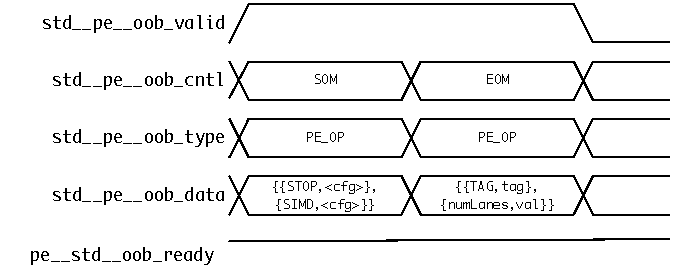
\includegraphics[width=0.7\textwidth]{stack_down_oob_wave_fig}
  \captionsetup{justification=centering, skip=10pt}
  \caption{Stack downstream OOB Bus}
  \label{fig:Stack downstream OOB Bus}
\end{subfigure}%

\bigskip

\begin{subfigure}{.9\textwidth}
  \centering
  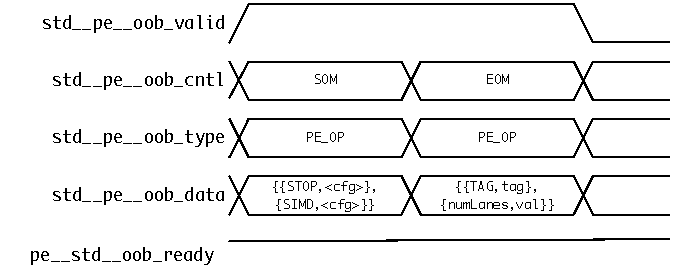
\includegraphics[width=0.7\textwidth]{stack_down_wave_fig}
  \captionsetup{justification=centering, skip=10pt}
  \caption{Stack downstream Data Bus}
  \label{fig:Stack downstream Data Bus}
\end{subfigure}%

\bigskip

\begin{subfigure}{.9\textwidth}
  \centering
  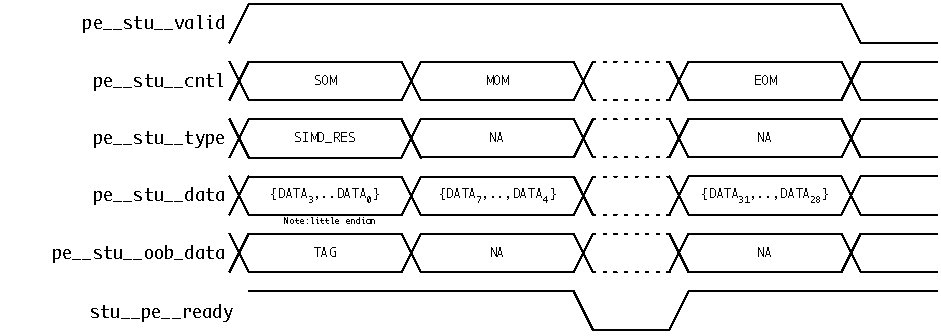
\includegraphics[width=0.7\textwidth]{stack_up_wave_fig}
  \captionsetup{justification=centering, skip=10pt}
  \caption{Stack upstream Bus}
  \label{fig:Stack upstream Bus}
\end{subfigure}%

\captionsetup{justification=centering, skip=16pt}
\caption{Stack Bus signalling}
\label{fig:Stack Bus signalling}
\end{figure}


\subsection{\ac{dram} Bus}
\label{sec:DRAM Bus}

The interface to the \ac{diram4} is similar to classic \ac{dram} interfaces with control signals including bank address and multiplexed page/cache address bus.
There are separate 2048-bit \ac{ddr} read and write databuses (see section \ref{sec:Very-Wide Bus}).
In total there are 4180 signals in the \ac{dram} interface.
Other than the wide databuses, the interface protocol is as described in \cite{tezzaron:diram4}.
A timing diagram showing a read and write to the \ac{diram4} are shown in figure \ref{fig:diram4Timing}.
\begin{figure}[!t]
\centering
\captionsetup{justification=centering}
\captionsetup{width=.9\linewidth}
\centerline{
\mbox{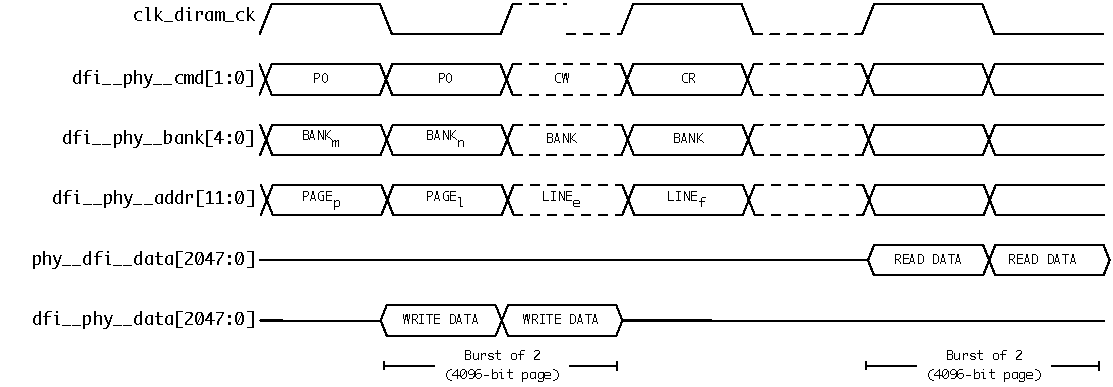
\includegraphics[width=.8\linewidth]{diram4TimingDiagram}}
}
\caption{Read and Write request to \ac{diram4} \cite{tezzaron:diram4}}
\label{fig:diram4Timing}
\end{figure}



The bandwidth of the \ac{dram} bus is designed to ensure data can be constantly maintained to the stack downstream bus.
Because an entire cacheline is accessed for each read request, there is an extreme case when back-to-back requests result in up to 32 \ac{dram} page opens commands.
It is possible that this sequence page opens could be followed by page closes resulting in a period when no useful data is being read from the \ac{diram4}.
This case is shown in figure \ref{fig:Worst case PO/PC sequence}.
\begin{figure}[!t]
\centering
\captionsetup{justification=centering}
\captionsetup{width=.9\linewidth}
\centerline{
\mbox{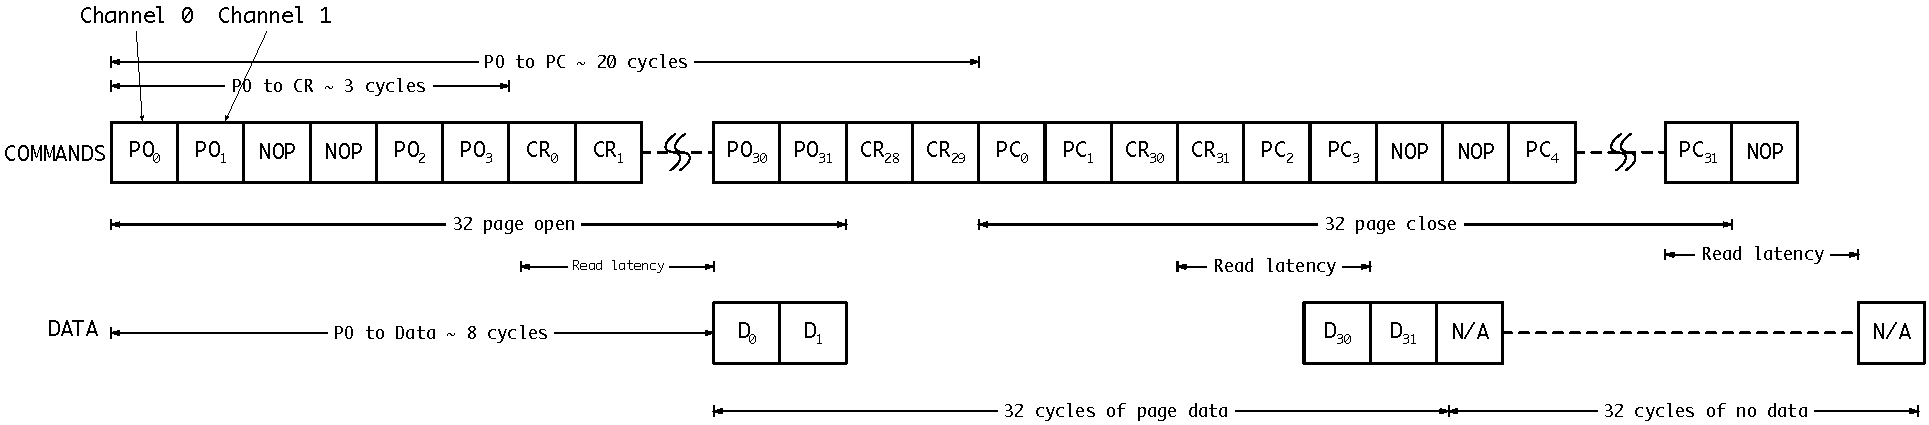
\includegraphics[width=1\linewidth]{worstCaseDiram4Read}}
}
\caption{Worst case PO/PC sequence}
\label{fig:Worst case PO/PC sequence}
\end{figure}
To accomodate this, the \ac{dram} bus has twice the raw bandwidth of the downstream stack bus. 
Therefore under this worst case scenario the higher bandwidth data from the \ac{diram4} must be buffered, as shown in figure \ref{fig:Worst case read path FIFO depth}.
In this case, per channel \SI[per-mode=symbol]{32}{\kilo\bit} \acp{fifo} must be placed in the read path as shown in figure \ref{fig:DRAM Read Path Buffering}.
These \acp{fifo} are instantiated in the managers memory read controller(s) as described in section \ref{sec:Memory Read Controller}.


\begin{figure}
\centering
\begin{subfigure}{.9\textwidth}
  \centering
  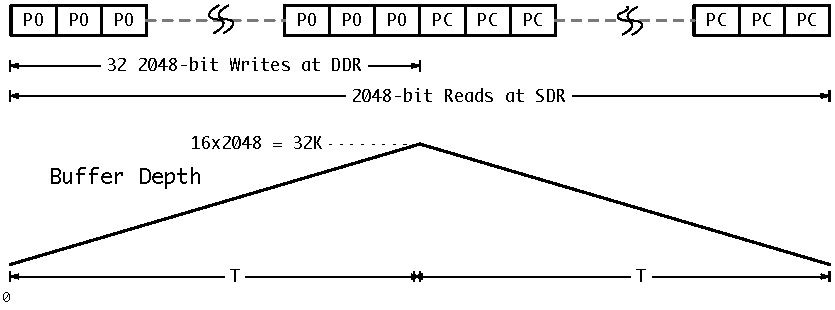
\includegraphics[width=0.7\textwidth]{readBufferDepth}
  \captionsetup{justification=centering, skip=0pt}
  \caption{Worst case read path FIFO depth}
  \label{fig:Worst case read path FIFO depth}
\end{subfigure}%

\bigskip

\vspace{-10pt}
\begin{subfigure}{.9\textwidth}
  \centering
  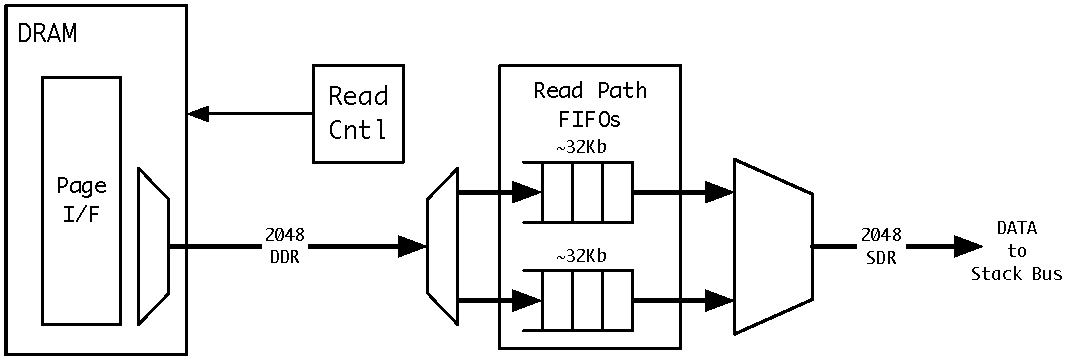
\includegraphics[width=0.75\textwidth]{readBufferBlockDiagram}
  \captionsetup{justification=centering, skip=6pt}
  \caption{Read path buffering diagram}
  \label{fig:Read path buffering diagram}
\end{subfigure}
\captionsetup{justification=centering, skip=16pt}
\caption{DRAM Read Path Buffering}
\label{fig:DRAM Read Path Buffering}
\end{figure}

\iffalse 
Each of the \ac{diram4} memories contain two channels with each channel containing 32 banks and each bank contains 4096 \SI[per-mode=symbol]{4}{\kilo\bit} pages.
\fi

% ----------------------------------------------------------------------------------------------------
\subsection{Manager Layer}
The Manager block is the main \ac{ssc} controller and the memory controller for the \ac{diram4} memory. 

The operations required to process an \ac{ann} are formed from individual instructions which are decoded by the Manager. 
These instructions (for more detail see section \ref{sec:Instructions}) are sub-divided into descriptors to describe memory read operations, processing engine operations, memory write operations and general system operations for synchronization. 
The manager reads these system instructions from an instruction memory, decodes the descriptors and configures the various blocks in the system.
The configuration includes:
\begin{itemize}
      \item initiating operand reads from \ac{dram}
      \item preparing the processing engine (\ac{pe}) to operate on the downstream stack bus operand streams
      \item prepare the result processing engine to take the resulting \ac{an} activations from the \ac{pe} via the upstream stack bus and write those results back to the \ac{dram}
      \item replicate the resulting \ac{an} activations to neighbor managers over the \ac{noc} for processing of other \ac{ann} layers
\end{itemize}

The most common instruction is to perform state calculation on a group of \acp{an}.
This instruction contains four descriptors (see figure \ref{fig:Instruction 4-tuple} and \ref{fig:Instruction Details}), an operation descriptor, two memory read descriptors and a memory write descriptor.
\begin{figure}[!t]
\centering
\captionsetup{justification=centering}
\captionsetup{width=.9\linewidth}
\centerline{
\mbox{
\includegraphics[width=.9\linewidth]{instruction4Tuple.jpg}}
}
\caption{Instruction 4-tuple}
\label{fig:Instruction 4-tuple}
\end{figure}


The operation descriptor describes the operations the \ac{pe} will perform, which typically includes a \ac{mac} to be performed by the \ac{stop} followed by a \ac{relu} function to be performed by the \ac{simd}.
The manager extracts the operation information, embeds the information in an \ac{oob} packet and sends the packet to the \ac{pe} over the downstream \ac{oob} bus.
The two memort read descriptors are used to define the memory locations of the downstream stack data buses. 
There is one memory read descriptor for each of the two operand streams in the execution lanes, one typically defines where the pre-synaptic weights are stored and one for where the pre-synaptic \ac{an} states are stored.
The architecture is designed to for an instruction to compute the state of multiple \acp{an} or for an individual \acp{an} state to be computed.
If a group of \acp{an} are computed, the pre-synaptic connection weights for the \acp{an} are stored interleaved and when read from \ac{dram} are directed to one of the streams of each of the execution lanes.
If a single \ac{an} is computed, the pre-synaptic connection weights for the \acp{an} are stored linearly and when read from \ac{dram} are directed to one of the streams of each of the execution lanes.
The pre-synaptic \ac{an} states are stored in row-major order and when read are broadcast to the other stream of each execution lane.



% ----------------------------------------------------------------------------------------------------
\subsection{Processing Engine Layer}
\label{sec:Processing Engine Layer}
The \ac{pe} contains two main processing modules, the \ac{stop} and the \ac{simd} block.
Both the \ac{stop} block and the \ac{simd} have 32 execution lanes. The execution lanes inside the \ac{stop} contain functions required to perform \ac{an} related operations.
The \ac{simd} will be based on the device described in \cite{schabel2014diss}.


The \ac{pe} is configured by the manager to perform operations on two operand data streams from the manager. 
The \ac{stop} is able to operate on this data directly from the manager at the full bandwidth rate of the stack bus and does not have to be stored in local \ac{sram} prior to processing. 
There is a small \ac{fifo} to provide buffering to allow asynchronous configuration of the \ac{stop} block and the source of the streaming data in the manager. 
The \ac{fifo} also allows the two argument streams in each of the execution lanes to wander with respect to each other and with respect to the other lanes.

The architecture is expandable to allow various functions to be provided in the \ac{stop}.
The current baseline implementation includes the \ac{mac} operation.
There is a \acp{mac} per execution lane allowing up to 32 simultaneous pre-synaptic \ac{an} $weight \cdot state$ computations on the two operands from the two streams in each execution lane.
These computations can be for a group of up to 32 \acp{an} or for a single \ac{an} as shown in figure \ref{fig:PE AN calculation}.

\begin{figure}
\centering
  \begin{subfigure}{.49\textwidth}
    \centering
    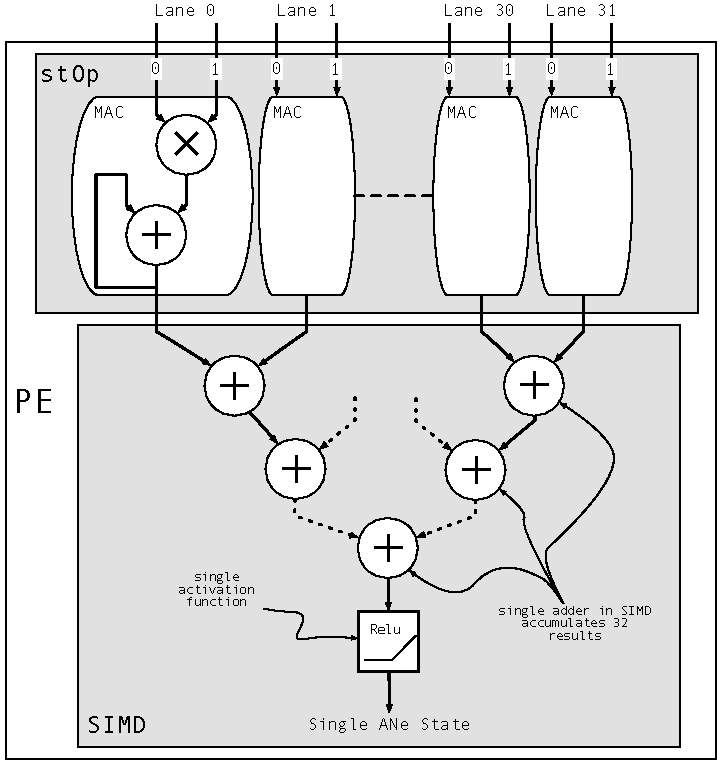
\includegraphics[width=0.9\textwidth]{singleANcalculation}
    \captionsetup{justification=centering, skip=10pt}
    \caption{Single ANe calculation}
    \label{fig:Single AN calculation}
  \end{subfigure}%
%\bigskip
  \begin{subfigure}{.49\textwidth}
    \centering
    \vspace{40pt}
    \includegraphics[width=0.9\textwidth]{groupANcalculation}
    \captionsetup{justification=centering, skip=10pt}
    \caption{Group ANe calculation}
    \label{fig:Group AN calculation}
  \end{subfigure}%
\vspace{-10pt}
\captionsetup{justification=centering, skip=16pt}
\caption{\ac{pe} \ac{an} calculation}
\label{fig:PE AN calculation}
\end{figure}

If it is for a group of \acp{an}, the \ac{simd} only has to perform the activation function on the 32 results from the \ac{stop}. 
If a single \ac{an} is being processed, the \ac{simd} must accumulate the result from each execution lanes \ac{stop} before applying the activation function.
The activation function currently implemented is the \ac{relu}.
The \ac{an} states can be sent back to the manager over the stack upstream bus or retained for further processing such as pooling or softmax calculations.

% ----------------------------------------------------------------------------------------------------
\subsection{Inter-Manager Communication}
\label{sec:Inter-Manager Communication}

During configuration and/or computations, it may be required to replicate data to other \acp{ssc}.
During \ac{an} computations, an \ac{ssc} only reads \ac{ann} weights and states from its local \ac{dram} and not \ac{dram} of other \acp{ssc}.
In some cases, such as fully connected layers and locally-connected layers with \ac{roi} overlap, the \ac{an} computation in an \ac{ssc} for layer $n$ may include \ac{an} states from layer $n-1$ which were computed in another \ac{ssc}.
In this case, when \acp{an} are being computed for layer $n-1$, the operation instruction contains information as to where the result should be written back for computing \acp{an} in layer $n$.
If a particular layer $n-1$ \ac{an} is required by another \ac{ssc} when computing a layer $n$ \ac{an}, the result is sent to all dependent \ac{ssc} via the \ac{noc}.
The instruction contains one or more storage descriptors (see section \ref{sec:Storage Descriptor}) that identify the destination of the operation result.
If the result must be replicated, there are multiple storage descriptors. When the result is returned by the \ac{pe}, the manager examines the storage descriptors and determines which \ac{ssc} the result should be sent.
The manager creates an \ac{noc} header which includes information on all the destination \acp{ssc}. 
This is encoded as a 64-bit field although to provide extensibility the \ac{noc} header supports a multicast group. 
The multiple storage descriptors and the result data are placed in the data portion of the \ac{noc} packet.
As the packet traverses the \ac{noc}, it is replicated to outgoing ports based on the destination bit field.
When the destination \ac{ssc} receives the packet, it extracts the storage descriptor and writes the data to its local \ac{dram}.
The \ac{noc} packet format can be seen in figure \ref{fig:NoC packet format}.
This inter-manager communication is provided by an \ac{noc} with all managers connected in a mesh as shown in figure \ref{fig:Mesh}.
\begin{figure}[!t]
% the [] contains position info e.g. [!t] means here
\centering
\captionsetup{justification=centering}
\centerline{
\mbox{\includegraphics[width=.5\linewidth]{Mesh}}
}
\caption{\ac{noc} manager connectivity}
\label{fig:Mesh}
\end{figure}

\begin{figure}[!t]
\centering
\captionsetup{justification=centering}
\captionsetup{width=.75\linewidth}
\centerline{
\mbox{\includegraphics[width=.9\linewidth]{nocpacket}}
}
\vspace{-10pt}
\caption{\ac{noc} packet format}
\label{fig:NoC packet format}
\end{figure}


When computing an \ac{ann} across multiple processing sub-systems, often \ac{an} activation data must be shared between these \ac{ssc}s. The \ac{ssc} includes the \ac{dram} port, the manager and the \ac{pe}. 
An \ac{noc} within each management block communicates with each adjacent manager using a mesh network. This \ac{noc} has a forwarding table that can be reconfigured to provide more efficient routing for a given processing step.

Each manager has an integrated \ac{noc} module that has four ports. 
The managers in the middle of the array use all four ports to connect to adjacent managers.
The managers in the corners of the array connect to two adjacent managers.
The managers at the edges connect to three adjacent managers.
The host is connected to one (or more) of the managers at one edge of the array. 

% ----------------------------------------------------------------------------------------------------
\section{Summary}
\label{sec:Overview Summary}

A control and data flow diagram of the stack showing the 64 sub-system columns can be seen in figure \ref{fig:FlowDiagram}.
\begin{figure}[!t]
% the [] contains position info e.g. [!t] means here
\centering
\captionsetup{justification=centering}
\centerline{
\mbox{\includegraphics[width=.8\linewidth]{FlowDiagram.jpg}}
}
\caption{System Flow Diagram}
\label{fig:FlowDiagram}
\end{figure}

\label{sec:Configuration, Command and Data Flow}

One of the primary objectives was to ensure the system can maintain the required average bandwidth (see table \ref{tab:Bandwidth and Storage Design Requirements}) whilst operating directly out of \ac{dram} over a range of pre-synaptic fanins.
To achieve this the system decodes instructions and concurently sends configuration information to various system functions.
It concurrently pre-fetchs and pipelines data to absorb the latencies associated with \ac{dram}.
All system functions pipeline their configuration data to ensure the main processing pipeline is not starved of data and/or operations.
This parallelism allows this system to constantly stream data whilst results from previous operations are being processed, broadcast to other \acp{ssc} and written back to \ac{ssc} memory.
The instructions, the structures for describing the operations and the structures describing how data is retrieved and stored have been architected to provide extensibility.
A detailed description of the instruction architecture and data structures is given in chapter \ref{sec:System Operations}.
The baseline \ac{ann} described in table \ref{tab:Layer Configuration} was used to define a collection of presynaptic fanin tests and the average bandwidth achieved from those tests were used to ensure the average bandwidth is maintained.
The results of those tests can be seen in chapter \ref{sec:Results}.


The second primary objective was to determine if a useful, extensible \ac{3dic} system could be designed employing a customized \ac{3ddram}.
The \ac{3ddram} employed was the \ac{diram4} and estimated areas were extracted from data provided by Tezzaron\textregistered~\cite{patti2014}.
The feasibility of the customizations were made with consultation with Tezzaron\textregistered.
The physical details for the \ac{rtl} design of the primary modules are given in chapter \ref{sec:Detailed System Description}.
The overall area details with respect to the \ac{3dic} stack are shown in chapter \ref{sec:Results}.






\chapter{System Operations}
\label{sec:System Operations}

As mentioned in Chapter \ref{sec:System Overview}, an \ac{ssc} has 32 execution lanes allowing the simultaneous processing of up to 32 \acp{an}.
When processing a group of \acp{an} the basic operations to determine their states are:
\begin{outline}
  %\lbbcleanspace{20pt}
  \lbbcleanspace
  \1 Manager streams the states of the pre-synaptic \acp{an} to the \ac{pe}
  \1 Manager streams the weights of the pre-synaptic connections to the \ac{pe}
  \1 Each execution lane in the \ac{pe} operates directly on the two argument streams using the \ac{stop} block
  \1 The \ac{pe} \ac{simd} block takes the 32 results from the \ac{stop} block and performs the activation function to generate the \ac{an} states
  \1 The \ac{pe} \ac{simd} packetizes the \ac{an} states and sends the packet to the manager
  \1 The manager replicates the \ac{an} state data over the \ac{noc} to any dependent \acp{ssc}
  \1 If the local \ac{ssc} is dependent on the result, the manager saves the \ac{an} state data in local \ac{ssc} \ac{dram}
\end{outline}

Although the primary focus of this work is effective use of a novel \ac{3ddram} along with an expansive system to process \acp{ann}, a complete system needs to also provide support features for tasks such as downloading the \ac{ann} parameters to memory from a host system and a host system also needs to download new inputs and upload \ac{ann} outputs.
This work has created a system and an infrastructure to include these support tasks.
Although not all of the features required for an actual final product have been included in this work's design and verification effort,  the infrastructure required to easily add the missing features has been provided.
This work has developed an instruction architecture to support and describe the operations associated with the processing of an \ac{ann} along with the support tasks required when employing this work in a product implementation.

\iffalse

The manager's primary responsibility is to decode instructions and descriptors and :

\begin{outline}
    \1 Instruction decode
    \1 Internal Configuration messaging
    \1 Operand read
    \1 Result write
    \1 Host to \ac{ssc} and \ac{ssc} to \ac{ssc} communication
\end{outline}


The \ac{pe} has three major blocks:

\begin{outline}
    \1 Streaming operation function (\ac{stop})
      \2 Processes data from the manager on-the-fly without storing in local \ac{sram}
    \1 \ac{simd}
      \2 processes the data from the \ac{stop} before returning data to the manager
    \1 DMA/local memory controller
      \2 transfer configuration data to \ac{pe} controller or to store \ac{stop} results to a small local \ac{sram} which can be used for access by \ac{simd} or by the \ac{stop} function
\end{outline}

\fi
% ----------------------------------------------------------------------------------------------------
% ----------------------------------------------------------------------------------------------------
\section{Instructions}
\label{sec:Instructions}

An instruction is coarse grained in as much as it provides the information to perform all the operations associated with a high level task.
The manager is responsible for instruction decode and coordinating the various data flows and configuration of the modules throughout the \ac{ssc}.
The \ac{pe} is responsible for the main algorithm operations using a combination of its \ac{stop} and \ac{simd} blocks.
The information in the instruction provides the information to control these finer grained functions within the manager and the \ac{pe} along with the various system support tasks.

To provide the fine grained information, an instruction is partitioned into sub-instructions called descriptors.
An instruction can contain one or more descriptors and each of these descriptors contains the information to control a specific operation(s) within the \ac{ssc} to perform the high level task.
For example, to process a group of \acp{an}, the instruction contains a descriptor to communicate where the pre-synaptic \ac{an} states are stored, another to communicate where the connection weights are stored, another describes what activation function should be used and another where in memory the resulting \ac{an} states should be stored.

% ----------------------------------------------------------------------------------------------------
\subsection{Instruction Types}
\label{sec:Instruction Types}
There are two instruction types currently defined, a \textbf{{\textcolor{black}{configuration}}} instruction and a \textbf{\textcolor{black}{compute}} instruction.
The configuration instruction has been defined to deal with synchronization and data downloads and uploads which includes \ac{ann} parameters and input, \ac{ssc} instructions, \ac{simd} and \ac{stop} operation pointers and \ac{simd} instructions.
The compute instruction has been defined to deal with computing the states of a group of \acp{an}.
Although this work's focus has been on the compute instruction -- as it has the most influence on system performance -- configuration instructions have been defined and tested to provide an extensible system.
\iffalse
\begin{outline}
  \lbbcleanspace
   \1 \ac{ann} parameters and input
   \1 \ac{ssc} instructions
   \1 \ac{simd} and \ac{stop} operation pointers
   \1 \ac{simd} instructions
\end{outline}
Typically an instruction contains information to process a group of \acp{an} but there are other instruction types to synchronize.
A group can be anywhere from one to 32 \acp{an} and is based on the number of execution lanes in the \ac{ssc} (see Section \ref{sec:Processing a group of ANes}) and how the user partitions the \ac{ann} across the available \acp{ssc}.
\fi

A generic instruction is an n-tuple where the tuple elements are descriptors and the number of descriptors can vary based on the high level task being performed. 
These descriptors are decoded and used to configure the various functions in the \ac{ssc} that will take part in completing the instruction. 
The contents of a single descriptor may be sent to multiple functions and in some cases the manager doesn't even parse the contents of the descriptor but immediately passes it to a dependent function.
This allows the system to concurrently prepare for the tasks involved with the instruction.


\subsection{Compute Instruction}
\label{sec:Compute Instruction}

The compute instruction typically contains four descriptors for configuring the tasks associated with processing a group of \acp{an}.
The instruction can be seen in Figure \ref{fig:Instruction (4-tuple example)} and includes: 
\begin{itemize}
  %\lbbcleanspace
  \item Operation descriptor containing:
    \begin{itemize}
      \item \ac{stop} operation
      \item \ac{simd} operation
      \item Number of active lanes
      \item Operand Vector length
    \end{itemize}
  \item Two memory read descriptors containing:
    \begin{itemize}
        \item Addresses for the pre-synaptic \ac{an} states and connection weights for the two argument streams to the \ac{pe}
        \item Read data to execution lane multiplex method (broadcast/vectored)
    \end{itemize}
  \item Memory write descriptor containing:
    \begin{itemize}
      \item \ac{dram} address for \ac{an} states
    \end{itemize}
\end{itemize}
\iffalse
\begin{figure}[!t]
\centering
\captionsetup{justification=centering}
\captionsetup{width=.9\linewidth}
\centerline{
\mbox{\includegraphics[width=.9\linewidth]{instruction4Tuple}}
}
\caption{Typical compute instruction (4-tuple)}
\label{fig:Instruction (4-tuple example)}
\end{figure}
\fi
\begin{figure}[!t]
  % the [] contains position info e.g. [!t] means here
  \centering
    \captionsetup{justification=centering, skip=10pt}
    \vspace{10mm}
    \begin{bytefield}[bitwidth=0.49em, endianness=big]{80}
      %\bitheader{0,32,64,96,128} \\
      %\begin{rightwordgroup}{\scriptsize Option Cycle}
        \colorbitbox{desc!40}{20}{\scriptsize Operation descriptor\\ \vspace{-0em}(MAC+ReLu)} & \colorbitbox{desc!40}{20}{\scriptsize Read descriptor\\ \vspace{-0em}(Input ROI)} & \colorbitbox{desc!40}{20}{\scriptsize Read descriptor \\ \vspace{-0em}(pre-synaptic \ac{an} states)} & \colorbitbox{desc!40}{20}{\scriptsize Write descriptor\\ \vspace{-0em}(store \ac{an} states)} 
      %\end{rightwordgroup}  \\
    \end{bytefield}
\caption{Typical compute instruction (4-tuple)}
\label{fig:Instruction (4-tuple example)}
\end{figure}


The descriptor also employs an n-tuple format where the elements contain configuration options required by the operation.
The option elements within a descriptor are a two-tuple with option and associated value and are referred to as option tuples.
These option tuples include a type and value, which contain information such as storage descriptor pointer (see Section \ref{sec:Storage Descriptor}), \ac{pe} operations and the number of operands.
The length of the value field is currently eight bits or 24-bits. The 24-bit value field is referred to as an extended tuple and is currently used for memory address, number of operands and configuration options.
In Figure \ref{fig:descriptorTuple} we see the format of a 5-tuple operation descriptor and a list of option types is shown in Table \ref{tab:Option tuple functions}.
%It should be noted that not all option tuple type are currently used in the system but were provided for expansibility.

\iffalse
\begin{figure}[!t]
\centering
\captionsetup{justification=centering}
\captionsetup{width=.9\linewidth}
\centerline{
\mbox{\includegraphics[width=.9\linewidth]{descriptorTuple}}
}
\caption{Operation descriptor (5-tuple example)}
\label{fig:descriptorTuple}
\end{figure}
\fi


\begin{figure}[!t]
  % the [] contains position info e.g. [!t] means here
  \centering
  \captionsetup{justification=centering}

  \begin{minipage}{1\textwidth}
    \centering
    \begin{minipage}{0.85\textwidth}
      \centering
      \captionsetup{justification=centering}
      \captionsetup{width=.9\linewidth}
      \centerline{
      \mbox{\includegraphics[width=.9\linewidth]{descriptorTuple}}
      }
      \vspace{-2mm}
      \caption{Operation descriptor (5-tuple example)}
      \label{fig:descriptorTuple}
    \end{minipage}
    \begin{minipage}{0.85\textwidth}
        \vspace{5mm}
        \begin{adjustbox}{width=1\textwidth}
            \footnotesize
            \begin{tabular}{ |c|c|c|c|  }
              \hline
              \rowcolor{gray!50}
              \multicolumn{4}{|c|}{Source} \\
              \hline
              \rowcolor{gray!25}
              Type & Type Code & extd &  Value Description  \\
              \hline
              NOP                              &    0   &  N&  \acl{nop} \\
              source                           &    1   &  N&  Used to define the source of any data, such as memory or \ac{pe}  \\
              target                           &    2   &  N&  Used to define the target for any data, such as memory or \ac{pe}  \\
              transfer type                    &    3   &  N&  How data will be directed, vector or broadcast                    \\
              number of lanes                  &    4   &  N&  number of active execution lanes used in operation \\
              \ac{stop} pointer                &    5   &  N&  pointer to \ac{pe} \ac{stop} operation table in \ac{pe} controller \\
              \ac{simd} pointer                &    6   &  N&  pointer to \ac{pe} \ac{simd} instruction memory  \\
              Memory storage descriptor        &    7   &  Y&  pointer to storage descriptor used in memory read or write \\
              num of arg0 operands             &    8   &  Y&  number of operands sent to execution lane stream 0\\
              num of arg1 operands             &    9   &  Y&  number of operands sent to execution lane stream 1\\
              num of return packets            &    10  &  Y&  number of response packets generated by PE \\
              config sync                      &    11  &  Y&  Synchronization \\
              config data                      &    12  &  Y&  Data transfers\\
              status                           &    13  &  Y&  status information \\
              \hline
            \end{tabular}
        \end{adjustbox}
        \captionof{table}{Option tuple functions}
        \label{tab:Option tuple functions}
    \end{minipage}
  \end{minipage}
\end{figure}


To pull it all together, Figure \ref{fig:Instruction Details} demonstrates a four-tuple compute instruction with details shown for each of the descriptors.
Figure \ref{fig:Instruction and Descriptors} shows the compute instruction which contains three 4-tuple and one 5-tuple descriptors.
The memory write descriptor shows two storage option elements which indicates the resulting \ac{an} states need to be saved in the memory of two \acp{ssc}.
The waveform in Figure \ref{fig:Instruction memory waveform} is from the verification environment and shows the instruction as it is read out of the manager's instruction memory.
The waveform also shows an example of the common interface signaling described in Section \label{sec:Common Bus Signalling} with the signals \texttt{wum\textunderscore\textunderscore wud\textunderscore\textunderscore icntl} and \texttt{wum\textunderscore\textunderscore wud\textunderscore\textunderscore dcntl} being used to delineate the instruction and descriptors respectively.
As can be seen in Figure \ref{fig:Instruction memory waveform}, the instruction memory transfers three descriptor elements per cycle shown on the bus signals \texttt{wum\textunderscore\textunderscore wud\textunderscore\textunderscore option\textunderscore type} and \texttt{wum\textunderscore\textunderscore wud\textunderscore\textunderscore option\textunderscore value}.
\\
Note: The signal name convention used between blocks in the \ac{rtl} is <src>\textunderscore\textunderscore <dest>\textunderscore\textunderscore <signal\textunderscore\textunderscore  name>. In Figure \ref{fig:Instruction memory waveform},~ \texttt{wum} and \texttt{wud} refer to ``work unit memory'' and ``work unit decode''
which correspond to the manager instruction memory and instruction decoder respectively.

\begin{figure}
\centering
  \begin{subfigure}{.95\textwidth}
    \centering
    \mbox{\includegraphics[width=1\linewidth]{instructionAndDescriptors}}
    \captionsetup{justification=centering, skip=6pt}
    \caption{Compute instruction and descriptors}
    \label{fig:Instruction and Descriptors}
  \end{subfigure}%

\bigskip

  \vspace{-35pt}
  \begin{subfigure}{1\textwidth}
    \centering
    \vspace{40pt}
    \includegraphics[width=0.95\textwidth]{instructionWaveform}
    \captionsetup{justification=centering, skip=10pt}
    \caption{Instruction memory waveform}
    \label{fig:Instruction memory waveform}
  \end{subfigure}%
%\vspace{-10pt}
\captionsetup{justification=centering, skip=16pt}
\caption{Compute Instruction details}
\label{fig:Instruction Details}
\end{figure}



% ----------------------------------------------------------------------------------------------------
\subsubsection{Accessing of Pre-synaptic \ac{an} states and connection weights}
\label{sec:AccessingANStates}

A part of the research is determining how to store the \ac{ann} input and parameters in such a way as to effectively make use of main \ac{dram} bandwidth. 
To provide parameters for the up to 32 execution lanes within the \ac{pe}, the \ac{an} parameters are stored in consecutive address locations. 
With one read to the \ac{dram}, we access 128 words. This provides four weights for each of the 32 \acp{an} being processed. 
These weights are sent to each lane of the \ac{pe} over four cycles. 
We will discuss memory efficiency later, but by taking advantage of the multiple \ac{dram} banks along with pre-fetching and buffering, we are able to make very efficient use of the available bandwidth.

Providing the pre-synaptic \ac{an} states to a particular \ac{an} presents us with an interesting problem.
\Acp{dnn} are represented by layers of \acp{an} whose pre-synaptic neurons are from the previous layer. These previous layers represent the input to a given layer with the first layer's input being the actual input to the \ac{ann}.
For the sake of generality, the \ac{ann} input array elements are considered as \ac{an} states.
Any given \ac{an} operates on a \ac{roi} within the input array. In the case of fully-connected layers, the entire input is the \ac{roi}. 
In the case of locally-connected layers, the \ac{roi} is a portion of the input array. 
Figure \ref{fig:roiStorage} shows an input to a \ac{ann} layer in the form of a 2-D array along with the \ac{roi} of two locally-connected \acp{an}.
\begin{figure}[!t]
\centering
\captionsetup{justification=centering}
\captionsetup{width=.9\linewidth}
\centerline{
\mbox{\includegraphics[width=.9\linewidth]{roiStorage.jpg}}
}
\caption{ROI Storage}
\label{fig:roiStorage}
\end{figure}

The various connection weights are stored in multiple contiguous sections. However, it's not possible to arrange the pre-synaptic \ac{an} states in the locally-connected \ac{roi} in such a way that each \ac{an}'s \ac{roi} can be stored in contiguous memory locations. 
Assuming the input array is stored in row-major order, a locally-connected \ac{roi} is drawn from disjoint sections of memory. 
These disjoint sections contain a number of \ac{an} states, in this case 14, and the sections are separated by a gap of a number of memory addresses. 
When the parameters are accessed while performing a particular operation, the memory controller within the manager must be informed of the start address and the lengths of the sections and gaps. 
In practice groups of \acp{an} share a common \ac{roi}, so often when reading an \ac{roi} from the \ac{dram} it is broadcast across a group of execution lanes.
The read efficiency problem is solved by again taking advantage of the \ac{dram}s banks and pages.
To describe the reading of a locally-connected \ac{roi}, this work proposes a data structure called a ``storage descriptor'' to describe the \ac{roi} storage locations.

\subsubsection{Storage Descriptor}
\label{sec:Storage Descriptor}

Although disparate groups of \acp{an} may have different start addresses for their \acp{roi}, a commonality is observed in the \ac{roi} section lengths and gaps. So for each \ac{an} group, the group's \ac{roi} starting address is stored along with a pointer to a common set of section lengths/gaps. This structure is termed a storage descriptor.

This storage descriptor contains, among other things, the start address of the \ac{roi} and a pointer to a section/gap descriptor. Many storage descriptors point to a common section/gap descriptor. This avoids having to have a unique section/gap descriptor for each \ac{an} group.

Figure \ref{fig:storageDescriptor} shows the structure of the storage descriptor. The \ac{sod}, \ac{mod} and \ac{eod} are used to delineate each storage descriptor in memory.

\begin{figure}[!t]
\centering
\captionsetup{justification=centering}
\captionsetup{width=.9\linewidth}
\centerline{
\mbox{\includegraphics[width=.9\linewidth]{storageDesc.jpg}}
}
\caption{Storage Descriptor}
\label{fig:storageDescriptor}
\end{figure}

% ----------------------------------------------------------------------------------------------------
\subsubsection{Writing \ac{an} state results to memory}
\label{sec:writingANStates}

When the \ac{pe} has processed the group of \acp{an}, the new \ac{an} states are sent back to the manager and stored in \ac{dram} in the row-major array format described earlier.
\iffalse
A significant difference taken advantage of is that for any given operation, the system is writing far less than is being read. For example, the \ac{roi} and parameters are usually vectors that exceed 100 elements and in many cases many more. When an operation is complete, in almost all cases one word per lane is written back to main memory. 
Now that sounds like writing back has a very small impact on performance, but with \acp{dram} that's not always true.
\fi
When an operation is complete, in almost all cases one word per lane is written back to \ac{dram}.
Considering a \ac{dram} page contains 128 words, the system typically writes a quarter of a page and this is a relatively inefficient use of \ac{dram} bandwidth. 
However, the pre-synaptic fanin typically far exceeds 100 elements and in the baseline \ac{an} shown in Table \ref{tab:Baseline Layer Configuration} the average fanin is \num 1650.
So the read-to-write ratio is very high and the inefficient write has little impact on the overall performance.

As discussed in Section \ref{sec:Inter-Manager Communication}, in many cases the results have to be provided not only to the local \ac{ssc} \ac{dram} but also to other \acp{ssc} memory. 
This is handled by examining the write storage descriptors and if at least one storage descriptor address references another \ac{ssc}'s memory, all the write storage descriptors in the instruction are included in the \ac{noc} packet (see Figure \ref{fig:NoC packet format}).

% ----------------------------------------------------------------------------------------------------
% ----------------------------------------------------------------------------------------------------
\iffalse
\section{PE Operations}
\label{sec:PE Operations}

% ----------------------------------------------------------------------------------------------------
\subsection{Streaming Operations (\ac{stop})}
\label{sec:streamingOps}
The operations performed by the \ac{stop} are primarily multiple-accumulate with a transfer to the \ac{simd} or to local memory.

Even though the baseline system focuses on the \ac{an} multiply-accumulate followed by a ReLu activation function, the system has built in flexibility into the \ac{stop} function to allow other functions to be added

In most cases, the \ac{stop} module will operate on the \ac{an} state and weights provided by the manager and provide the result to the \ac{simd}.
% ----------------------------------------------------------------------------------------------------
\subsection{SIMD}
\label{sec:SIMD}

The \ac{simd} is a 32-lane processor with some built-in special functions, such as the ReLu operation.

The \ac{simd} will take the result provided by the \ac{stop} and perform a ReLu. The result will, in most cases, then transmitted back to the manager.

% ----------------------------------------------------------------------------------------------------
\subsection{Configuration}
\label{sec:peConfiguration}

To configure these operations, two pointers are sent to the \ac{pe}. These pointers index into a small local memory which provides a program counter (\ac{pc}) to the function to be performed by the \ac{simd} and a configuration entry for the operation to be performed by the \ac{stop}.

The \ac{pe} is able to perform its operation concurrently on 32 lanes. However, there are cases when less than 32 lanes will be employed. This may occur if the number of \acp{an} being processed is not modulo-32. In this case, the manager provides the number of lanes being processed for any given operation. In addition, the length of the vector of operands is also sent to the \ac{pe} by the manager.
\fi

\subsection{Configuration Instruction}
\label{sec:Configuration Instruction}

The configuration instruction is used for :
\begin{itemize}
  \lbbcleanspace
    \item Data transfer
    \begin{itemize}
      \item Download Instructions from host to \ac{ssc} manager instruction memory
      \item Download Sync group data from host to \ac{ssc} manager 
      \item Download \ac{ann} parameters and input from host to \ac{ssc} memory
      \item Upload \ac{ann} output to host from \ac{ssc} memory
    \end{itemize}
  \item System synchronization
    \begin{itemize}
      \item Send a sync message to a group of \acp{ssc}
      \item Wait for sync messages from a group of \acp{ssc} or host
      \item Pause instruction fetch
      \item Flush \ac{pe} operations
    \end{itemize}
\end{itemize}

The configuration instruction contains one descriptor and there are two configuration types which are characterized by the descriptor option tuple contents.
All configuration descriptors start with a configuration option tuple. There are two configuration tuple types, sync and data.
The sync and data option types are extended types that have a 24-bit option value.
The 24-bit option value is used to define one of up to eight mode registers, each of which defines the type of configuration operation and various options.
The configuration option tuple can be seen in Figure \ref{fig:Configuration tuple}.

The data transfer configuration instruction is shown in Figure \ref{fig:Data transfer instruction}. The descriptor is a 2-tuple with a configuration data option type and a storage option type.
The sync configuration instruction is shown in Figure \ref{fig:Sync instruction} and the descriptor is a 1-tuple with a sync configuration option type.

\begin{figure}[h]
\centering

  %\begin{minipage}{1\textwidth}
  %\begin{subfigure}{1\textwidth}
    \centering
    \captionsetup{justification=centering, skip=10pt}
    \begin{bytefield}[bitwidth=1.49em, endianness=big]{32}
      \bitheader{0,20,21,23,24,31} \\
      %\begin{rightwordgroup}{\scriptsize Option Cycle}
        \colorbitbox{optiontype!40}{8}{\scriptsize Sync or Data} & \colorbitbox{optionvalue!40}{3}{\scriptsize Mode Register ID} & \colorbitbox{optionvalue!40}{21}{\scriptsize Mode register value } 
      %\end{rightwordgroup}  \\
    \end{bytefield}
    \captionsetup{justification=centering, skip=9pt}
    \vspace{-2mm}
    \captionof{figure}{Configuration tuple}
    \label{fig:Configuration tuple}
  %\end{subfigure}%
  %\end{minipage}
\end{figure}

\begin{figure}[h]
\centering

  \begin{subfigure}{.85\textwidth}
    \centering
    \mbox{\includegraphics[width=1\linewidth]{dataTransferInstruction}}
    \captionsetup{justification=centering, skip=6pt}
    \caption{Data transfer instruction }
    \label{fig:Data transfer instruction}
  \end{subfigure}%

\bigskip

  \vspace{-35pt}
  \begin{subfigure}{0.85\textwidth}
     \centering
     \vspace{40pt}
     \includegraphics[width=1\textwidth]{syncInstruction}
     \captionsetup{justification=centering, skip=10pt}
     \caption{Sync instruction }
     \label{fig:Sync instruction}
  \end{subfigure}%
  %\vspace{-10pt}
  \captionsetup{justification=centering, skip=16pt}
  \caption{Configuration instruction types}
  \label{fig:Configuration Instruction types}
\end{figure}

The data option value mode register \cite{standard2007jedec} defines the type of data transfer along with information to aid the transfer. 
The storage option type contains a storage descriptor pointer which specifies the address of memory transfers.
An overview of the configuration instructions is given in Sections \ref{sec:Data Transfer Instruction} and \ref{sec:Sync Instruction} with additional details in Section \ref{sec:Decoding Configuration Instructions}.

\subsubsection{Configuration Data Instruction}
\label{sec:Data Transfer Instruction}

There are currently four mode registers defined, an instruction download register, a sync group download register, a memory download register and a memory upload register.
The contents of the mode register specify the type of transfer, the size of the transfer and some additional flags.
When transferring to or from memory, an additional descriptor element contains a storage descriptor defining where the data should read or written.

\subsubsection{Configuration Sync Instruction}
\label{sec:Sync Instruction}

The option element is a sync option whose value contains a mode register.
There are currently four mode registers defined, a send, wait, pause and a flush register.
The contents of the send and wait mode register specify the group of \acp{ssc} to be synchronized. 
The send register causes a sync \ac{noc} packet to be sent to all \acp{ssc} in the group.
The wait register causes the manager to wait for a \ac{noc} sync packet to be received from all \acp{ssc} in the group.
The pause mode register causes the instruction fetch logic to pause the specified number of clock cycles.
The flush mode register causes the instruction fetch logic to wait for all outstanding \ac{pe} operations to be returned before continuing.

\subsection{Multiple Instruction Functions}
\label{sec:Multiple Instruction Functions}

When instructions or data are downloaded, in some cases there are tasks in the system that must be performed by chaining instructions together.
This is the case when downloading the \ac{pe} operation pointers and the \ac{simd} instructions.
In these cases, the host will have to first download the data to the \ac{ssc} local \ac{dram} in conjunction with a \ac{ssc} configuration download instruction.
The data is then transferred to the \ac{pe} using an operation instruction with the \ac{stop} configured as a \ac{nop} so the data will pass through the \ac{stop} with the small local \ac{sram} as the target. 
The \ac{pe} controller will then transfer the contents of the \ac{sram} to \ac{simd} instruction memory or the operation pointer memory.
As an example, loading the \ac{simd} instruction memory requires the procedure described in algorithm \ref{alg:Load SIMD Instruction memory}.

\begin{algorithm}
\caption{Load SIMD Instruction memory}
\label{alg:Load SIMD Instruction memory}
\begin{algorithmic}[1]
    %      inst       desc
    \State{// last compute instruction}
    \State \makebox[1.05cm][r]{COM:[}\makebox[0.25cm][r]{[}\makebox[0.85cm][r]{  op}\makebox[0.15cm][l]{:}\makebox[0.15cm][r]{[}\makebox[1.00cm][r]{stOp:}\makebox[1.25cm][l]{fpmac}\makebox[0.25cm][r]{,}\makebox[1.00cm][r]{simd:}\makebox[0.80cm][l]{relu }\makebox[0.25cm][r]{,}\makebox[1.65cm][r]{numop0:}\makebox[0.75cm][l]{<n>}\makebox[0.25cm][r]{,}\makebox[1.65cm][r]{numop1:}\makebox[1.00cm][l]{<n>  }\makebox[0.25cm][r]{]} \\
           \makebox[1.05cm][r]{     }\makebox[0.25cm][r]{[}\makebox[0.85cm][r]{  mr}\makebox[0.15cm][l]{:}\makebox[0.15cm][r]{[}\makebox[1.00cm][r]{ tgt:}\makebox[1.25cm][l]{std0 }\makebox[0.25cm][r]{,}\makebox[1.00cm][r]{txfr:}\makebox[0.80cm][l]{bcast}\makebox[0.25cm][r]{,}\makebox[1.65cm][r]{ lanes:}\makebox[0.75cm][l]{<l>}\makebox[0.25cm][r]{,}\makebox[1.65cm][r]{  StoD:}\makebox[1.00cm][l]{<ptr>}\makebox[0.25cm][r]{]} \\
           \makebox[1.05cm][r]{     }\makebox[0.25cm][r]{[}\makebox[0.85cm][r]{  mr}\makebox[0.15cm][l]{:}\makebox[0.15cm][r]{[}\makebox[1.00cm][r]{ tgt:}\makebox[1.25cm][l]{std1 }\makebox[0.25cm][r]{,}\makebox[1.00cm][r]{txfr:}\makebox[0.80cm][l]{vec  }\makebox[0.25cm][r]{,}\makebox[1.65cm][r]{ lanes:}\makebox[0.75cm][l]{<l>}\makebox[0.25cm][r]{,}\makebox[1.65cm][r]{  StoD:}\makebox[1.00cm][l]{<ptr>}\makebox[0.25cm][r]{]} \\
           \makebox[1.05cm][r]{     }\makebox[0.25cm][r]{[}\makebox[0.85cm][r]{  mw}\makebox[0.15cm][l]{:}\makebox[0.15cm][r]{[}\makebox[1.00cm][r]{ src:}\makebox[1.25cm][l]{stu  }\makebox[0.25cm][r]{,}\makebox[1.00cm][r]{txfr:}\makebox[0.80cm][l]{vec  }\makebox[0.25cm][r]{,}\makebox[1.65cm][r]{ lanes:}\makebox[0.75cm][l]{<l>}\makebox[0.25cm][r]{,}\makebox[1.65cm][r]{  StoD:}\makebox[1.00cm][l]{<ptr>}\makebox[0.25cm][r]{,}\makebox[1.00cm][r]{  StoD:}\makebox[1.00cm][l]{<ptr>}\makebox[0.25cm][r]{]} 
\\
    \State{//---------------------------------------- Start download ---------------------------------------- }
    \State{// make sure all compute instruction are complete}
    \State \makebox[1.05cm][r]{CFG:[}\makebox[0.25cm][r]{[}\makebox[0.85cm][r]{ cfg}\makebox[0.15cm][l]{:}\makebox[0.15cm][r]{[}\makebox[1.00cm][r]{sync:}\makebox[0.25cm][r]{[}\makebox[1.75cm][r]{flush}\makebox[0.25cm][r]{]}\makebox[0.25cm][r]{]}
    \State \makebox[1.05cm][r]{CFG:[}\makebox[0.25cm][r]{[}\makebox[0.85cm][r]{ cfg}\makebox[0.15cm][l]{:}\makebox[0.15cm][r]{[}\makebox[1.00cm][r]{sync:}\makebox[0.25cm][r]{[}\makebox[1.75cm][r]{send:}\makebox[0.25cm][r]{[}\makebox[1.00cm][l]{host }\makebox[0.25cm][r]{]}\makebox[0.25cm][r]{]}\makebox[0.25cm][r]{]}
    \State \makebox[1.05cm][r]{CFG:[}\makebox[0.25cm][r]{[}\makebox[0.85cm][r]{ cfg}\makebox[0.15cm][l]{:}\makebox[0.15cm][r]{[}\makebox[1.00cm][r]{sync:}\makebox[0.25cm][r]{[}\makebox[1.75cm][r]{wait:}\makebox[0.25cm][r]{[}\makebox[1.00cm][l]{host }\makebox[0.25cm][r]{]}\makebox[0.25cm][r]{]}\makebox[0.25cm][r]{]}
    \State{// Host sends release}
\\
    \State{// Host starts simd instruction download to SSC memory}
    \State{// Next SSC instruction prepares wr\textunderscore cntl for data from Host}
    \State \makebox[1.05cm][r]{CFG:[}\makebox[0.25cm][r]{[}\makebox[0.85cm][r]{ cfg}\makebox[0.15cm][l]{:}\makebox[0.15cm][r]{[}\makebox[1.00cm][r]{data:}\makebox[0.25cm][r]{[}\makebox[1.75cm][r]{mem\textunderscore dn:}\makebox[1.00cm][l]{<m>}\makebox[0.25cm][r]{,}\makebox[1.65cm][r]{  StoD:}\makebox[1.00cm][l]{<ptr>}\makebox[0.25cm][r]{]}
    \State \makebox[1.05cm][r]{CFG:[}\makebox[0.25cm][r]{[}\makebox[0.85cm][r]{ cfg}\makebox[0.15cm][l]{:}\makebox[0.15cm][r]{[}\makebox[1.00cm][r]{sync:}\makebox[0.25cm][r]{[}\makebox[1.75cm][r]{pause:}\makebox[0.25cm][r]{[}\makebox[1.00cm][l]{ind }\makebox[0.25cm][r]{]}\makebox[0.25cm][r]{]}\makebox[0.25cm][r]{]}
    \State{// fetch paused waiting for release, wr\textunderscore cntl ready for Host data}
    \State{// wr\textunderscore cntl releases fetch when data transfer complete}
    \State \makebox[1.05cm][r]{COM:[}\makebox[0.25cm][r]{[}\makebox[0.85cm][r]{  op}\makebox[0.15cm][l]{:}\makebox[0.15cm][r]{[}\makebox[1.00cm][r]{stOp:}\makebox[1.25cm][l]{ld\textunderscore simd}\makebox[0.25cm][r]{,}\makebox[1.00cm][r]{simd:}\makebox[0.80cm][l]{nop  }\makebox[0.25cm][r]{,}\makebox[1.65cm][r]{numop0:}\makebox[0.75cm][l]{<m>}\makebox[0.25cm][r]{]} \\
           \makebox[1.05cm][r]{     }\makebox[0.25cm][r]{[}\makebox[0.85cm][r]{  mr}\makebox[0.15cm][l]{:}\makebox[0.15cm][r]{[}\makebox[1.00cm][r]{ tgt:}\makebox[1.25cm][l]{std0}\makebox[0.25cm][r]{,}\makebox[1.00cm][r]{txfr:}\makebox[0.80cm][l]{bcast}\makebox[0.25cm][r]{,}\makebox[1.65cm][r]{ lanes:}\makebox[0.75cm][l]{1}\makebox[0.25cm][r]{,}\makebox[1.65cm][r]{  StoD:}\makebox[1.00cm][l]{<ptr>}\makebox[0.25cm][r]{]}
    \State{// manager sending instruction data to PE using compute operation with NOPs}
    \State{// flush PE to ensure instruction data complete}
    \State \makebox[1.05cm][r]{CFG:[}\makebox[0.25cm][r]{[}\makebox[0.85cm][r]{ cfg}\makebox[0.15cm][l]{:}\makebox[0.15cm][r]{[}\makebox[1.00cm][r]{sync:}\makebox[0.25cm][r]{[}\makebox[1.75cm][r]{flush}\makebox[0.25cm][r]{]}\makebox[0.25cm][r]{]}
    %\State \makebox[1.05cm][r]{CFG:[}\makebox[0.25cm][r]{[}\makebox[0.85cm][r]{ cfg}\makebox[0.15cm][l]{:}\makebox[0.15cm][r]{[}\makebox[1.00cm][r]{sync:}\makebox[0.25cm][r]{[}\makebox[1.75cm][r]{send:}\makebox[0.25cm][r]{[}\makebox[1.00cm][l]{host }\makebox[0.25cm][r]{]}\makebox[0.25cm][r]{]}\makebox[0.25cm][r]{]}
    %\State \makebox[1.05cm][r]{CFG:[}\makebox[0.25cm][r]{[}\makebox[0.85cm][r]{ cfg}\makebox[0.15cm][l]{:}\makebox[0.15cm][r]{[}\makebox[1.00cm][r]{sync:}\makebox[0.25cm][r]{[}\makebox[1.75cm][r]{wait:}\makebox[0.25cm][r]{[}\makebox[1.00cm][l]{host }\makebox[0.25cm][r]{]}\makebox[0.25cm][r]{]}\makebox[0.25cm][r]{]}
    \State{//---------------------------------------- end of download ---------------------------------------- }
\\
    \State{// continue with compute instructions}
    \State \makebox[1.05cm][r]{COM:[}\makebox[0.25cm][r]{[}\makebox[0.85cm][r]{  op}\makebox[0.15cm][l]{:}\makebox[0.15cm][r]{[}\makebox[1.00cm][r]{stOp:}\makebox[1.25cm][l]{fpmac}\makebox[0.25cm][r]{,}\makebox[1.00cm][r]{simd:}\makebox[0.80cm][l]{relu }\makebox[0.25cm][r]{,}\makebox[1.65cm][r]{numop0:}\makebox[0.75cm][l]{<n>}\makebox[0.25cm][r]{,}\makebox[1.65cm][r]{numop1:}\makebox[1.00cm][l]{<n>  }\makebox[0.25cm][r]{]} \\
           \makebox[1.05cm][r]{     }\makebox[0.25cm][r]{[}\makebox[0.85cm][r]{  mr}\makebox[0.15cm][l]{:}\makebox[0.15cm][r]{[}\makebox[1.00cm][r]{ tgt:}\makebox[1.25cm][l]{std0 }\makebox[0.25cm][r]{,}\makebox[1.00cm][r]{txfr:}\makebox[0.80cm][l]{bcast}\makebox[0.25cm][r]{,}\makebox[1.65cm][r]{ lanes:}\makebox[0.75cm][l]{<l>}\makebox[0.25cm][r]{,}\makebox[1.65cm][r]{  StoD:}\makebox[1.00cm][l]{<ptr>}\makebox[0.25cm][r]{]} \\
           \makebox[1.05cm][r]{     }\makebox[0.25cm][r]{[}\makebox[0.85cm][r]{  mr}\makebox[0.15cm][l]{:}\makebox[0.15cm][r]{[}\makebox[1.00cm][r]{ tgt:}\makebox[1.25cm][l]{std1 }\makebox[0.25cm][r]{,}\makebox[1.00cm][r]{txfr:}\makebox[0.80cm][l]{vec  }\makebox[0.25cm][r]{,}\makebox[1.65cm][r]{ lanes:}\makebox[0.75cm][l]{<l>}\makebox[0.25cm][r]{,}\makebox[1.65cm][r]{  StoD:}\makebox[1.00cm][l]{<ptr>}\makebox[0.25cm][r]{]} \\
           \makebox[1.05cm][r]{     }\makebox[0.25cm][r]{[}\makebox[0.85cm][r]{  mw}\makebox[0.15cm][l]{:}\makebox[0.15cm][r]{[}\makebox[1.00cm][r]{ src:}\makebox[1.25cm][l]{stu  }\makebox[0.25cm][r]{,}\makebox[1.00cm][r]{txfr:}\makebox[0.80cm][l]{vec  }\makebox[0.25cm][r]{,}\makebox[1.65cm][r]{ lanes:}\makebox[0.75cm][l]{<l>}\makebox[0.25cm][r]{,}\makebox[1.65cm][r]{  StoD:}\makebox[1.00cm][l]{<ptr>}\makebox[0.25cm][r]{,}\makebox[1.00cm][r]{  StoD:}\makebox[1.00cm][l]{<ptr>}\makebox[0.25cm][r]{]} 
\end{algorithmic}
\end{algorithm}




% ----------------------------------------------------------------------------------------------------
% ----------------------------------------------------------------------------------------------------
\section{Host Instructions}
\label{sec:Host Instructions}

The host is responsible for transferring \ac{ann} parameters and input data to the \ac{ssc} and for transferring \ac{ann} output data back to the host.
It is also responsible for downloading configuration data including \ac{ssc} instructions, \ac{pe} and \ac{simd} instructions and configuration tables such as storage pointer tables and \ac{pe}, \ac{stop} and \ac{simd} operation tables.

The host will use the \ac{noc} to carry the commands and data to accomplish the transfers.
The commands will employ the same option tuple method as described in Section \ref{sec:Configuration Instruction}.

A transfer of data to the \ac{ssc} can be solicited or unsolicited.
In the unsolicited case, the host initiates the transfer by sending the first \ac{noc} packet with two option tuples along with the first data as shown in Figure \ref{fig:Host transfer configuration packet}.
This first packet contains a configuration data option tuple (see Figure \ref{fig:Configuration tuple}) which contains a mode register used to define the type of transfer.
The second tuple has a storage descriptor pointer defining where in memory to write the data.
Once the first packet has been received, the \ac{ssc} expects only to receive data packets as shown in Figure \ref{fig:Host transfer data packet}.
In the solicited case, the transfer is initiated from a configuration data transfer instruction in which case the main controller receives the mode register and storage descriptor from the instruction decoder.
An example instruction can be seen in Figure \ref{fig:Data transfer instruction}.
In this case, the host will only send data packets as shown in Figure \ref{fig:Host transfer data packet}.
Additional information on the configuration data option tuple mode registers can be found in Sections \ref{sec:Memory download reg} and \ref{sec:Memory upload reg}.

In the case of a data download, the main controller sends the storage tuple to the memory write controller and indicates it's a \ac{dma}.
This will inform the memory write controller to expect further data packets and associate those with the current storage descriptor.
In the case of a data upload, the main controller will check the status of the instruction decode and if it has not been halted by a sync instruction, it will halt the instruction decoder.
The main controller then sends the storage tuple to the lane 0 memory read controller.

The data to be transferred is included in separate packets as shown in Figure \ref{fig:Host transfer data packet}.
For downloads, the host sends the data and the main controller passes the packets to the memory write controller.
In the case of reads, the main controller receives data from the memory read controller, packetizes the data and sends it to the host.
If the amount of data exceeds the 32 data word \ac{mtu} of the \ac{noc}, the data will be fragmented.




\begin{figure}[!t]
  % the [] contains position info e.g. [!t] means here
  \centering
  \captionsetup{justification=centering}

  \begin{minipage}{1\textwidth}
  %\begin{subfigure}{1\textwidth}
    \centering
    \captionsetup{justification=centering, skip=10pt}
    \begin{bytefield}[bitwidth=0.49em, endianness=big]{77}
      \bitheader{0,8,16,24,32,40,48,56,64,68,74,76} \\
      \begin{rightwordgroup}{\scriptsize Header}
        \bitbox{2}{\rotatebox{90}{\tiny SOM}} & \bitbox{7}{\scriptsize src} & \bitbox{2}{\tiny M} & \bitbox{1}{\rotatebox{90}{\tiny prio}} & \bitbox{64}{\tiny destination SSC bitfield} 
      \end{rightwordgroup}  \\
      \begin{rightwordgroup}{\scriptsize Option Cycle}
        \bitbox{2}{\rotatebox{90}{\tiny EOM}} & \bitbox{1}{} & \bitbox{4}{\tiny type} & \bitbox{3}{\tiny pyld\\ \vspace{-0em} type} & \bitbox{1}{} & \bitbox{1}{\tiny P\\ V} & \colorbitbox{optiontype!40}{8}{\tiny config\\ \vspace{-0em}data} & \colorbitbox{optionvalue!40}{3}{\tiny mem\\ dnld} & \colorbitbox{optionvalue!40}{21}{\tiny number of \\ bytes} & \colorbitbox{optiontype!40}{8}{\tiny storage\\ desc} & \colorbitbox{optionvalue!40}{6}{\tiny SSC ID} & \colorbitbox{optionvalue!40}{18}{\tiny storage descriptor\\ pointer}
      \end{rightwordgroup}  \\
      \begin{rightwordgroup}{\scriptsize Data Cycle}
        \bitbox{2}{\rotatebox{90}{\tiny MOM}} & \bitbox{1}{} & \bitbox{4}{\tiny type} & \bitbox{3}{\tiny pyld\\ \vspace{-0em} type} & \bitbox{1}{} & \bitbox{1}{\tiny P\\ V} & \bitbox{32}{\tiny Data} & \bitbox{32}{\tiny Data}
      \end{rightwordgroup}  \\
      \bitbox[]{76}{$\vdots$} \\[1ex]
      \begin{rightwordgroup}{\scriptsize Data Cycle}
        \bitbox{2}{\rotatebox{90}{\tiny EOM}} & \bitbox{1}{} & \bitbox{4}{\tiny type} & \bitbox{3}{\tiny pyld\\ \vspace{-0em} type} & \bitbox{1}{} & \bitbox{1}{\tiny P\\ V} & \bitbox{32}{\tiny Data} & \bitbox{32}{\tiny Data}
      \end{rightwordgroup}  \\
    \end{bytefield}
    \captionsetup{justification=centering, skip=9pt}
    \vspace{-0.5cm}
    \captionof{figure}{Host unsolicited download first \ac{noc} packet}
    \label{fig:Host transfer configuration packet}
  \end{minipage}

  \bigskip
  \vspace{0.5cm}

  \begin{minipage}{1\textwidth}
  %\begin{subfigure}{1\textwidth}
    \centering
    \captionsetup{justification=centering, skip=10pt}
    \begin{bytefield}[bitwidth=0.49em, endianness=big]{77}
      \bitheader{0,8,16,24,32,40,48,56,64,68,74,76} \\
      \begin{rightwordgroup}{\scriptsize Header}
        \bitbox{2}{\rotatebox{90}{\tiny SOM}} & \bitbox{7}{\scriptsize src} & \bitbox{2}{\tiny M} & \bitbox{1}{\rotatebox{90}{\tiny prio}} & \bitbox{64}{\tiny destination SSC bitfield} 
      \end{rightwordgroup}  \\
      \begin{rightwordgroup}{\scriptsize Data Cycle}
        \bitbox{2}{\rotatebox{90}{\tiny MOM}} & \bitbox{1}{} & \bitbox{4}{\tiny type} & \bitbox{3}{\tiny pyld\\ \vspace{-0em} type} & \bitbox{1}{} & \bitbox{1}{\tiny P\\ V} & \bitbox{32}{\tiny Data} & \bitbox{32}{\tiny Data}
      \end{rightwordgroup}  \\
      \bitbox[]{76}{$\vdots$} \\[1ex]
      \begin{rightwordgroup}{\scriptsize Data Cycle}
        \bitbox{2}{\rotatebox{90}{\tiny EOM}} & \bitbox{1}{} & \bitbox{4}{\tiny type} & \bitbox{3}{\tiny pyld\\ \vspace{-0em} type} & \bitbox{1}{} & \bitbox{1}{\tiny P\\ V} & \bitbox{32}{\tiny Data} & \bitbox{32}{\tiny Data}
      \end{rightwordgroup}  \\
    \end{bytefield}
    \captionsetup{justification=centering, skip=9pt}
    \vspace{-0.5cm}
    \captionof{figure}{Host transfer \ac{noc} data only packet}
    \label{fig:Host transfer data packet}
  \end{minipage}
\end{figure}


%The host transfer logic has not been implemented and will be covered in future work.


%% Lee
%% In dissertation, change 
%    section* to chapter 
%    subsection* to section
%    subsubsection* to subsection


% #######################################################################################################################################
\chapter{Detailed System Description}
\label{sec:Detailed System Description}

A detailed flow diagram and block diagram of the sub-system column can be seen in figures \ref{fig:DetailedFlowDiagram} and \ref{fig:DetailedBlockDiagram} respectively.
\begin{figure}[h]
% the [] contains position info e.g. [!t] means here
\centering
\captionsetup{justification=centering}
\captionsetup{width=.9\linewidth}
\centerline{
\mbox{\includegraphics[scale=0.5]{DetailedFlowDiagram}}
}
\center\caption{Sub-System Column (SSC) Flow Diagram}
\label{fig:DetailedFlowDiagram}
\end{figure}

\section{Manager}
\label{sec:manager}

A block diagram of the manager can be seen in figure \ref{fig:Manager block diagram}.
\begin{figure}[h]
\centering
\captionsetup{justification=centering}
\captionsetup{width=.9\linewidth}
\centerline{
\mbox{\includegraphics[width=1\linewidth]{Manager}}
}
\center\caption{Manager block diagram}
\label{fig:Manager block diagram}
\end{figure}

\subsection{System controller}
\label{sec:System controller}

The system controller is responsible for initialization and general system configuration.
A block diagram can be seen in figure \ref{fig:System controller}.

\begin{figure}[h]
% the [] contains position info e.g. [!t] means here
\centering
\captionsetup{justification=centering}
\captionsetup{width=.9\linewidth}
\centerline{
\mbox{\includegraphics[scale=1.5]{systemControllerBlockDiagram}}
}
\center\caption{System controller}
\label{fig:System controller}
\end{figure}

\subsubsection{Initial Boot}
\label{sec:Initial Boot}

The system controller is responsible for performing the initial \ac{bootp} process.
This involves quiescing the system after reset and downloading the initial boot instructions from the host.

After reset, the controller keeps the instruction fetch logic disabled and expects unsolicited \ac{noc} packets from the host which contain the initial boot code.
The host will unsolicitedly send the \ac{bootp} code over the \ac{noc} to each \ac{ssc}.
The controller in each \ac{ssc} decodes the \ac{noc} packets and writes the data directly into instruction memory.
Currently each \ac{noc} \ac{mtu} packet contains 16 instruction memory entries (see figure \ref{fig:Host boot code packet}).
The number of initial instruction entries is hard-coded but it is anticipated a standard on-chip protocol such as \ac{jtag} will be used to set initial \ac{bootp} configuration.
Once the host has sent the \ac{bootp} code, each \ac{ssc} controller releases its instruction fetch block.

It is anticipated that the initial \ac{bootp} code will not contain operational instructions but only configuration instructions to download configuration tables, the \ac{pe} \ac{simd} instruction memory and the \ac{ann} parameters.
For example, to download the \ac{ann} parameters, the \ac{bootp} instructions will include a configuration sync and a configuration data download.

The first \ac{bootp} instruction will be a configuration sync sent to the host to indicate the initial \ac{bootp} is complete and \ac{ann} parameters are ready to be received.
After the configuration sync is sent to the host, the configuration data instruction will prepare the \ac{ssc} to receive data from the host and the host will then start sending configuration data. 
The size of the data is known by both the \ac{ssc} via the instruction and the host.
The \ac{ann} parameters can be downloaded using multiple downloads.
Once \ac{ann} parameters and system tables are downloaded, the last instruction can be another configuration data instruction download to load operational code.

\begin{figure}[h]
  \vspace{5mm}
  \begin{minipage}{1\textwidth}
  %\begin{subfigure}{1\textwidth}
    \centering
    \captionsetup{justification=centering, skip=10pt}
    \begin{bytefield}[bitwidth=0.49em, endianness=big]{77}
      \bitheader{0,8,16,24,32,40,48,56,64,68,74,76} \\
      \begin{rightwordgroup}{\scriptsize Unicast Bitfield header}
        \bitbox{2}{\rotatebox{90}{\tiny SOM}} & \bitbox{7}{\scriptsize src} & \bitbox{2}{\tiny M} & \bitbox{1}{\rotatebox{90}{\tiny prio}} & \bitbox{64}{\tiny destination SSC bitfield} 
      \end{rightwordgroup}  \\
      \begin{rightwordgroup}{\scriptsize Data Cycle}
        \bitbox{2}{\rotatebox{90}{\tiny MOM}} & \bitbox{1}{} & \bitbox{4}{\tiny type} & \bitbox{3}{\tiny pyld\\ \vspace{-0em} type} & \bitbox{1}{} & \bitbox{1}{\tiny P\\ V} & \bitbox{7}{\tiny NA} & \bitbox{57}{\tiny Instruction memory entry}
      \end{rightwordgroup}  \\
      \bitbox[]{76}{$\vdots$} \\[1ex]
      \begin{rightwordgroup}{\scriptsize Data Cycle}
        \bitbox{2}{\rotatebox{90}{\tiny EOM}} & \bitbox{1}{} & \bitbox{4}{\tiny type} & \bitbox{3}{\tiny pyld\\ \vspace{-0em} type} & \bitbox{1}{} & \bitbox{1}{\tiny P\\ V} & \bitbox{7}{\tiny NA} & \bitbox{57}{\tiny Instruction memory entry}
      \end{rightwordgroup}  \\
    \end{bytefield}
    \captionsetup{justification=centering, skip=9pt}
    \vspace{-0.5cm}
    \captionof{figure}{Host boot code download \ac{noc} packet}
    \label{fig:Host boot code packet}
  \end{minipage}
\end{figure}

\subsection{Instruction Decoder}
\label{sec:Instruction Decoder}

In figure \ref{fig:Manager block diagram}, instructions are read from WU memory by the WU fetch block and the output of the memory is passed to the WU decoder block.

\subsubsection{Compute Instructions}
\label{sec:Decoding Compute Instructions}

The operation descriptor is decoded and a \ac{stop} pointer and a \ac{simd} \ac{pc} pointer are extracted. 
A sequential tag is generated and along with the \ac{stop} and \ac{simd} pointers and immediately sent to the \ac{pe} inside an \ac{oob} control packet.
The \ac{stop} pointer specifies what streaming operation is to take place on the data directly streamed to the \ac{pe}. 
The SIMD pointer is essentially a \ac{pc} counter that the \ac{simd} will jump to to process the result from the \ac{stop}.
The \ac{pe} will immediately start preparing for downstream oeprand data.
If the \ac{simd} operation ncludes result data being returned to the manager, the tag will be included in the upstream result data packet.

The memory read descriptors are decoded to identify the target memory read controller and the storage descriptor pointer directed to the appropriate memory read block.
There is a memory read block associated with each of the operand streams and are responsible for generating memory requests and directing the \ac{dram} data to all the execution lane streams.
A request block inside the memory read block immediately start pre-fetching the memory data by sending memory requests to the \ac{dram}.
A stream block inside the memory read block immediately starts waiting for data from the \ac{dram} and will direct \ac{dram} data to the appropriate execution lane.

The memory write descriptor is decoded and the storage descriptor pointer extracted and along with the tag are sent to the return data processor. The tag is sent to match with the returned data.
Currently the system only allows in-order data but the tag is provided for extensibility.

At this point all the blocks that take part in a compute operation on a group of \acp{an} are perforiming the various tasks.
As mentioned in section \ref{sec:Common Bus Signalling}, the inputs to many blocks employ \acp{fifo}. 
This allows blocks to pipeline tasks to absorb any latencies, they also allow blocks to start sending data to a destination block before that block has been configured to receive the data.
The \ac{fifo} will assert a flow control signal until the block is ready to receive.
In practice, the instruction decode logic batch decodes up to eight instructions and sends descriptor contents to dependent blocks where they are also pipelined.

\subsubsection{Configuration Instructions}
\label{sec:Decoding Configuration Instructions}

The configuration instructions are responsible for :
\begin{outline}
 \1 performing synchronization between the \ac{ssc} and other \acp{ssc} or the host system.
 \1 performing data download and upload operations
\end{outline}

The configuration packets are broken into two types, configuration data and configuration sync.
\iffalse
Currently the sync instruction has been implemented.
It is assumed at this point that adequate infrastructure and extensibility has been built into the system to allow implementation without adding significant amouts of logic.
\fi

The configuration instruction contains a single descriptor with one, two or three option tuples.

The sync instruction descriptor contains a single configuration sync option tuple. The 24-bit option value contains a 3-bit mode register identifier and a 21-bit mode register.
There are currently four mode registers defined, "Send", "Wait", "Pause" and "Flush". Each register has fields specific to the mode as seen in figure \ref{fig:Sync instruction}.

The data configuration instruction descriptor contains a configuration data option tuple and a storage descriptor tuple and optionally a target tuple. 
The configuration data option value is 24-bits with a 3-bit mode register identifier and a 21-bit mode register.
There are currently four mode registers defined, "instruction download", "sync group download", "memory download" and "memory upload". Each register has fields specific to the mode as seen in figure \ref{fig:Data transfer instruction}.

\paragraph{Sync Send}

The register fields can be seen in register \ref{reg:Sync Send mode register}.
The decoder sends the sync option tuple to the system controller.
A sync \ac{noc} packet is constructed based on the register contents sent over the \ac{noc}.
If the group pointer enable bit is set, the system conntroller uses the pointer to index into a 64 table. 
Each table entry is a 64-bit bitfield indicating which \acp{ssc} are a part of the group.
If the all flag is set, the sync packet will be sent to all \acp{ssc}.
if the host flag is also set, the host bit in the \ac{noc} packet will be set.
\begin{register}{H}{Sync Send mode register}{}%{0x250} name=example
  \label{reg:Sync Send mode register}
  % sizes 
  %\tiny 	
  %\scriptsize 	
  %\footnotesize
  %\small 	
  %\normalsize 	
  %\large 	
  %\Large 	
  %\LARGE 	
  \vspace{-20pt}
  \regfield{{\scriptsize Mode Reg ID         }}{ 3}{21}{000}%
  \regfield{{\scriptsize Not used            }}{12}{ 9}{{NA}}%
  \regfield{{\scriptsize Group Pointer enable}}{ 1}{ 8}{{en}}%
  \regfield{{\scriptsize Sync Group pointer  }}{ 6}{ 2}{{gPtr}}%
  \regfield{{\scriptsize Send to all SSCs    }}{ 1}{ 1}{{{\tiny all}}}%
  \regfield{{\scriptsize Send to host        }}{ 1}{ 0}{{{\tiny  host}}}%
  %\center\caption{Sub-System Column (SSC) Block Diagram}
  %\reglabel{Reset}\regnewline%
\end{register}

\paragraph{Sync Wait}

The register fields can be seen in register \ref{reg:Sync Send mode register}.
The decoder sends the sync option tuple to the system conntroller.
The instruction decoder will stop processing any more instructions until the release signal is asserted from the system conntroller.
The wait option informs the system conntroller to start expecting sync send packets from other \acp{ssc} and/or the host.
Based on the register values, the system conntroller will assert the release signal to the instruction decoder only once sync send packets have been received from all specified sources.
If the group pointer enable bit is set, the system conntroller uses the pointer to index into a 64 table. 
Each table entry is a 64-bit bitfield indicating from which \acp{ssc} a sync send packet should be received.
If the all flag is set, all sync send packets are expected from all \acp{ssc}.
if the host flag is also set, a sync send packet is expected from the host.
\begin{register}{H}{Sync Wait mode register}{}%{0x250} name=example
  \label{reg:Sync Wait mode register}
  \vspace{-20pt}
  \regfield{{\scriptsize Mode Reg ID         }}{ 3}{21}{001}%
  \regfield{{\scriptsize Not used            }}{12}{ 9}{{NA}}%
  \regfield{{\scriptsize Group Pointer enable}}{ 1}{ 8}{{en}}%
  \regfield{{\scriptsize Sync Group pointer  }}{ 6}{ 2}{{gPtr}}%
  \regfield{{\scriptsize Receive from all SSCs    }}{ 1}{ 1}{{{\tiny all}}}%
  \regfield{{\scriptsize Receive from host        }}{ 1}{ 0}{{{\tiny  host}}}%
  %\center\caption{Sub-System Column (SSC) Block Diagram}
  %\reglabel{Reset}\regnewline%
\end{register}


\paragraph{Sync Pause}

The register fields can be seen in register \ref{reg:Sync Pause mode register}.
The decoder sends the sync option tuple to the system conntroller and ceases decoding instructions.
If the indefinitely flag is set, instruction decode will not restart until the release signal is asserted from the system conntroller, otherwise the decoder will wait a number of clock cycles specified by the count field and then restart decoding instructions.
\begin{register}{H}{Sync Pause mode register}{}%{0x250} name=example
  \label{reg:Sync Pause mode register}
  \vspace{-10pt}
  \regfield{{\scriptsize Mode Reg ID         }}{ 3}{21}{010}%
  \regfield{{\scriptsize Wait <count> cycles }}{12}{ 9}{{count}}%
  \regfield{{\scriptsize Not used            }}{ 8}{ 1}{{NA}}%
  \regfield{{\scriptsize Indefinitely        }}{ 1}{ 8}{{Ind}}%
  %\center\caption{Sub-System Column (SSC) Block Diagram}
  %\reglabel{Reset}\regnewline%
\end{register}

\paragraph{Sync Flush}

There are currently no fields implemented in the sync flush register.
This instruction is designed to pause instruction decode until all outstanding commands sent to the \ac{pe} have been returned to the manager.
The decoder sends the sync option tuple to the return data processor and pauses processing instructions.
When the return data processor receives all outstanding tags, it asserts a release signal to the decoder.

%\begin{register}{H}{Sync Flush mode register}{}%{0x250} name=example
%  \label{reg:Sync Flush mode register}
%  \vspace{-10pt}
%  \regfield{{\scriptsize Mode Reg ID         }}{ 3}{21}{011}%
%  \regfield{{\scriptsize Not used            }}{21}{ 0}{{NA}}%
%  %\center\caption{Sub-System Column (SSC) Block Diagram}
%  %\reglabel{Reset}\regnewline%
%\end{register}

\paragraph{Instruction download}

The register fields can be seen in register \ref{reg:Inst dnld mode register}.
The decoder sends the data option tuple to the system controller.
The system controller will ensure the fetch and decode blocks are disabled and then expects to receive the number of instruction entries from the host over the \ac{noc}.
Once the instruction memory is loaded, the system controller will enable the fetch and decode loagic.
\begin{register}{H}{Instruction download mode register}{}%{0x250} name=example
  \label{reg:Inst dnld mode register}
  % sizes 
  %\tiny 	
  %\scriptsize 	
  %\footnotesize
  %\small 	
  %\normalsize 	
  %\large 	
  %\Large 	
  %\LARGE 	
  \vspace{-10pt}
  \regfield{{\scriptsize Mode Reg ID         }}{ 3}{21}{000}%
  \regfield{{\scriptsize Number of entries  }}{13}{ 8}{{number}}%
  \regfield{{\scriptsize Not used            }}{ 7}{ 1}{{NA}}%
  \regfield{{\scriptsize continue            }}{ 1}{ 0}{{en}}%
  %\center\caption{Sub-System Column (SSC) Block Diagram}
  %\reglabel{Reset}\regnewline%
\end{register}

\paragraph{Sync group table download}

The register fields can be seen in register \ref{reg:Sync grp dnld mode register}.
The decoder sends the data option tuple to the system controller.
The system controller will ensure the fetch and decode blocks are disabled and then expects to receive the number of sync groups from the host over the \ac{noc}.
The group table entry is 64-bits and eight are contained in an \ac{noc} packet.
Once the sync group table is loaded, the system controller will enable the fetch and decode loagic.
\begin{register}{H}{Sync group table download mode register}{}%{0x250} name=example
  \label{reg:Sync grp dnld mode register}
  % sizes 
  %\tiny 	
  %\scriptsize 	
  %\footnotesize
  %\small 	
  %\normalsize 	
  %\large 	
  %\Large 	
  %\LARGE 	
  \vspace{-10pt}
  \regfield{{\scriptsize Mode Reg ID         }}{ 3}{21}{001}%
  \regfield{{\scriptsize Not used            }}{ 5}{16}{{NA}}%
  \regfield{{\scriptsize Number of groups    }}{ 8}{ 8}{{number}}%
  \regfield{{\scriptsize Not used            }}{ 7}{ 1}{{NA}}%
  \regfield{{\scriptsize continue            }}{ 1}{ 0}{{en}}%
  %\center\caption{Sub-System Column (SSC) Block Diagram}
  %\reglabel{Reset}\regnewline%
\end{register}

\paragraph{Memory download}
\label{sec:Memory download reg}

The register fields can be seen in register \ref{reg:Mem dnld mode register}.
The decoder sends the data option tuple to the system controller.
The system controller will ensure the fetch and decode blocks are disabled and then expects to receive the number of bytes from the host over the \ac{noc}.
As each data packet is received, it is passed to the memory write controller along with the storage descriptor for writing to \ac{dram}.
\begin{register}{H}{Memory download mode register}{}%{0x250} name=example
  \label{reg:Mem dnld mode register}
  % sizes 
  %\tiny 	
  %\scriptsize 	
  %\footnotesize
  %\small 	
  %\normalsize 	
  %\large 	
  %\Large 	
  %\LARGE 	
  \vspace{-10pt}
  \regfield{{\scriptsize Mode Reg ID         }}{ 3}{21}{010}%
  \regfield{{\scriptsize Number of bytes     }}{21}{ 0}{{number}}
  %\center\caption{Sub-System Column (SSC) Block Diagram}
  %\reglabel{Reset}\regnewline%
\end{register}

\paragraph{Memory upload}
\label{sec:Memory upload reg}

The register fields can be seen in register \ref{reg:Mem upld mode register}.
The decoder sends the data option tuple to the system controller.
The system controller will ensure the fetch and decode blocks are disabled.
The controller sends the storage descriptor and target option tuples to the the stream 0 memory read controller. 
The read controller generates read requests to the \ac{dram} and sends the corresponding read data to the system controller.
The system controller the data and embeds the data in an \ac{noc} packet and send it to the host.
The data is fragmented and sent using multiple data \ac{noc} packets.
\begin{register}{H}{Memory upload mode register}{}%{0x250} name=example
  \label{reg:Mem upld mode register}
  % sizes 
  %\tiny 	
  %\scriptsize 	
  %\footnotesize
  %\small 	
  %\normalsize 	
  %\large 	
  %\Large 	
  %\LARGE 	
  \vspace{-10pt}
  \regfield{{\scriptsize Mode Reg ID         }}{ 3}{21}{011}%
  \regfield{{\scriptsize Number of bytes     }}{21}{ 0}{{number}}
  %\center\caption{Sub-System Column (SSC) Block Diagram}
  %\reglabel{Reset}\regnewline%
\end{register}

\iffalse
\subsubsection{Argument Decode}
\label{sec:argumentDecode}
The instruction also includes memory read descriptors. These descriptors include storage descriptor pointers that point to a storage descriptor stored in local memory that encodes where data should be read from for the two operand streamss in each execution lane.
As soon as the memory read descriptor target option is decoded, the read storage descriptor pointers are passed to the \acp{mrc}.
The \acp{mrc} read the actual storage descriptor from their local memory and immediately start sending read commands to the memory via a \ac{mmc}. 
The \ac{mmc} is not shown in the diagram but essentially takes the memory read requests and converts them into the \ac{dram} read protocol.

As soon as read data is sent back to the \ac{mrc} via the \ac{mmc}, that data is aligned with the downstream bus and sent to the 32 Streaming Operations inside the PE.
\fi


\subsection{\Acf{mmc}}
\label{sec:MMC}

The \ac{mmc} is responsible for taking read requests from the two \acp{mrc} and write requests from the \ac{mwc}.

The read requests the \ac{mmc} receives from the \acp{mrc} includes channel, bank, page and cacheline addresses. 
The request also contains an operation identifier.
The write requests from the \ac{mwc} includes channel, bank, page and cacheline addresses. 

The \ac{mmc} processes the three requestors providing a small priority to write requests.
In addition, the \ac{mmc} processes all read erquests associated with an operation before processing requests from the next operation.
This is because memory requests are pre-fetched and memory requests for the next operation will be received before the \ac{mrc} has streamed data for the previous operation.
This avoids the case where a request from the next operation could block a request from the rpevious operation causing a deadlock.

The \ac{mmc} does not reorder requests to improve \ac{dram} efficiency. 
the \ac{mmc} does keep track of open pages within banks to avoid unnecessary page open and page close commands.
It should be noted that refresh has yet to be implemented but this is not anticipated to be a significant impact and will eb done in future work.

The \ac{mmc} ensures the \ac{dram} protocol is observed and this was verified using the Tezzaron \ac{diram4} verilog models during simulation.


\subsection{\Acf{mrc}}
\label{sec:MRC}

The \ac{mrc} is provided with multiple option tuples by the decoder block, a storage descriptor pointer, the number of execution lanes, the target for read data and the transfer type.
The \ac{mrc} contains the \ac{dram} read \acp{fifo} described in section \ref{sec:DRAM Bus} and shown in figure \ref{fig:Worst case PO/PC sequence}.
A block diagram of the \ac{mrc} can be seen in figure \ref{fig:MRC block diagram}.
\begin{figure}[h]
\centering
\captionsetup{justification=centering}
\captionsetup{width=.9\linewidth}
\centerline{
\mbox{\includegraphics[width=1\linewidth]{mrcBlockDiagram}}
}
\center\caption{MRC block diagram}
\label{fig:MRC block diagram}
\end{figure}

The \ac{mrc} is one of the most complicated blocks in the system, it is also the largest but mainly because of the size of the data path \acp{fifo}.
There are two \ac{mrc} blocks instantiated in the manager, one for stream 0 and one for stream 1 in the execution lanes.

The \ac{mrc} uses the storage descriptor to identify the start address of the data and how the address should be incremented.
The \ac{sdp} block contains a request block and a stream block.
The request block uses the storage descriptor pointer to index into a small memory containing the actual storage descriptor. 
As described in section \ref{sec:Storage Descriptor}, the storage descriptor itself contains a start address and a pointer to a table containing consequtive and jump fields.
The starting address and consequtive/jump fields allow the request generator to make disjoint memory requests based on the \ac{roi} of the data. 
If the \ac{roi} is contiguous in memory, then there is one consequitive field and no jump field.

The request block generates memory requests based on the storage descriptor contents and number of lanes and sends the requests to the \ac{mmc}.
The request information is also sent to the stream block.
As the request block processes the storage descriptor start address and consequtive/jump fields it also send the information to the stream block.

The stream block is responsible for taking the 2048-bit memory data from the \ac{mmc} and directing words to each execution lane.
As the data is returned from the \ac{mmc}, it is placed in a channel 0 \ac{fifo} and a channel 1 \ac{fifo}. 
The stream block has a per execution lane index module each of which generates an index to the channel and word.
The index is used to multiplex the data to the execution lane stream.
The per execution lane index module is required to account for bank and page boundaries in the \ac{roi} as described in sections \ref{sec:AccessingANStates} and \ref{sec:Storage Descriptor}.
The lane index module uses the storage descritpor information to generate a memory location address which includes channel, bank, page and word addresses.
The location address is them matched to the request at the head of the two request \acp{fifo}, and it a match occurs, the data is passed to the execution lane bus.
If there is no match, the index module requests the request and data \acp{fifo} are read. The request control \ac{fsm} will ony read the \ac{fifo} if all lane index modules make a read request.
This is done because as data is stored in memory, if the data crosses a bank, page or cacheline boundary the execution lanes must be allowed to get out of sync.


\subsection{\Acf{rdp}}
\label{sec:RDP}
The \ac{rdp} is responsible for taking the result data from the \ac{pe} and determining which \ac{ssc} it should be stored (see figure \ref{fig:RDP block diagram}).

\begin{figure}[h]
\centering
\captionsetup{justification=centering}
\captionsetup{width=.9\linewidth}
\centerline{
\mbox{\includegraphics[width=0.85\linewidth]{rdpBlockDiagram}}
}
\center\caption{Result data processor}
\label{fig:RDP block diagram}
\end{figure}

The \ac{rdp} receives a descriptor from the decoder which includes storage descriptor information and the tag associated with an operation sent to the \ac{pe}.
The information is stored in a \ac{fifo} and as data is returned to the manager over the upstream stack bus, the \ac{rdp} matches the return data tag with the head of the \ac{fifo}.
Currently the return data is in order but to support an expansive architecture the tag is provided to and checked by the \ac{rdp}.

When the data is matched to the tag, the \ac{rdp} examines all the storage descriptor pointers. The pointers include \ac{ssc} index in the \acp{msb} and the \ac{rdp} constructs an \ac{ssc} bit-field.
Once the descriptors have been parsed, if one of the destinations is the local \ac{ssc} \ac{dram}, the \ac{rdp} passed the descriptor and data to the system conntroller which in turn passes it to the \ac{mwc}.
If the destination(s) include other \acp{ssc}, the \ac{rdp} provides the \ac{ssc} bitfield along with the data to the \ac{noc}.


\subsection{\Acf{mwc}}
\label{sec:MWC}

The \acf{mwc} receives data from two sources, the \ac{noc} via the system conntroller and the \ac{rdp}.
The \ac{mwc} uses the storage descriptor provided with the data to identify the write address.
The \ac{mwc} does not store the data immediately, it places the data in a small crude cache which has enough storage for two pages per channel.
A block diagram of the \ac{mwc} can be seen in figure \ref{fig:MWC block diagram}.
\begin{figure}[h]
\centering
\captionsetup{justification=centering}
\captionsetup{width=.9\linewidth}
\centerline{
\mbox{\includegraphics[width=0.85\linewidth]{mwcBlockDiagram}}
}
\center\caption{MWC block diagram}
\label{fig:MWC block diagram}
\end{figure}
As data is received from the \ac{rdp} or \ac{noc}, the addresses are compared to the cache entry and if page address match occurs and the corresponding word is invalid, the data is stored in the cache.
If a page miss occurs, the contents of one of the entries is written to memory and the new data stored in the cache.

This crude cache was provided for two reasons, first even though write efficiency was not anticipated to be an issue, as described in section \ref{sec:writingANStates}, it was anticipated that the addresses from multiple operations may occur in consequive address and by coalescing data would make writes more efficient.
The more important reason was to provide expansibility and by accounting for a small cache future work, such as host data downloads would have less of an impact on logic area.


\section{Processing Engine}
\label{sec:pe}

A block diagram of the \ac{pe} can be seen in figure \ref{fig:PE block diagram}.
\begin{figure}[h]
\centering
\captionsetup{justification=centering}
\captionsetup{width=.9\linewidth}
\centerline{
\mbox{\includegraphics[width=1\linewidth]{PE}}
}
\center\caption{PE block diagram}
\label{fig:PE block diagram}
\end{figure}

\subsection{Configuration}
\label{sec:peConfiguration}

The manager sends configuration information to the \ac{pe} over the downstream \ac{oob} bus.
The \ac{oob} packet contains option tuples used by the \ac{pe} controller to configure functions within the \ac{pe}.
The controller extracts the \ac{stop} and \ac{simd} operation pointers from the appropriate option tuple value.
The \ac{stop} pointer is used to point to a local \ac{stop} configuration which contains the various configuration data required by the \ac{stop} function.
The configuration data includes:
\begin{outline}
    \1 \ac{stop} operation type
    \1 Number of active execution lanes
    \1 Source of the argument data, which can be downstream data from the manager or from the small local \ac{sram}
    \1 Destination of the result data, which can be the \ac{simd} and/or the small local \ac{sram}
\end{outline}
Once the information is provided to the \ac{stop} block and the pointer provided to the \ac{simd}, the operation is immediately started.
Currently only \ac{stop} and \ac{simd} pointer option tuples are used.
An example of the downstream \ac{oob} transactions can be seen in figure \ref{fig:Downstream OOB transactions}. This example shows both normal and extended option tuples.

\begin{figure}[h]
  % the [] contains position info e.g. [!t] means here
  \centering
  \captionsetup{justification=centering}

  \begin{minipage}{1\textwidth}
    \centering
    \captionsetup{justification=centering, skip=10pt}
    \begin{minipage}[t]{1\textwidth}
      \begin{minipage}[t]{1\textwidth}
        \begin{center}
          \begin{bytefield}[bitwidth=0.49em, endianness=big]{38}
            \bitheader{0, 31, 37} \\
            \bitbox{2}{\rotatebox{90}{\tiny SOM}} & \bitbox{4}{\tiny type} & \colorbitbox{optiontype!40}{8}{\tiny option \\ \vspace{-0em}type} & \colorbitbox{optionvalue!40}{8}{\tiny option \\ \vspace{-0em}value} & \colorbitbox{optiontype!40}{8}{\tiny option \\ \vspace{-0em}type} & \colorbitbox{optionvalue!40}{8}{\tiny option \\ \vspace{-0em}value}   \\
            \bitbox{2}{\rotatebox{90}{\tiny MOM}} & \bitbox{4}{\tiny type} & \colorbitbox{optiontype!40}{8}{\tiny extd option \\ \vspace{-0em}type} & \colorbitbox{optionvalue!40}{24}{\tiny option \\ \vspace{-0em}value} \\
            \bitbox[]{38}{$\vdots$} \\[1ex]                                                                                                                                                                          
            \bitbox{2}{\rotatebox{90}{\tiny EOM}} & \bitbox{4}{\tiny type} & \colorbitbox{optiontype!40}{8}{\tiny option \\ \vspace{-0em}type} & \colorbitbox{optionvalue!40}{8}{\tiny option \\ \vspace{-0em}value} & \colorbitbox{optiontype!40}{8}{\tiny option \\ \vspace{-0em}type} & \colorbitbox{optionvalue!40}{8}{\tiny option \\ \vspace{-0em}value}   \\
          \end{bytefield}
        \end{center}
      \end{minipage}
  \end{minipage}
  \begin{minipage}{1\textwidth}
      \centering
      \begin{minipage}[t]{0.28\textwidth}
        \vspace{1mm}
        \centering
        \begin{adjustbox}{width=1\textwidth}
            \footnotesize
            \begin{tabular}{ |c|c|  }
              \hline
              \rowcolor{gray!50}
              \multicolumn{2}{|c|}{Type} \\
              \hline
              \rowcolor{gray!25}
              type[3:0] & Description  \\
              \hline
              2     & Operation configuration \\
              other & NA \\
              \hline
            \end{tabular}
        \end{adjustbox}
      \end{minipage}
      \vspace{-2mm}
      \center\caption{Downstream OOB data transactions}
      \label{fig:Downstream OOB transactions}
    \end{minipage}
    \begin{minipage}[t]{1\textwidth}
      \vspace{7mm}
      \centering
      %\begin{adjustbox}{width=1\textwidth}
        \centering
        \includegraphics[scale=0.35]{stack_down_oob_waveform}
      %\end{adjustbox}
      \captionsetup{justification=centering, skip=10pt}
      \captionof{figure}{Downstream OOB simulation waveform}
      \label{fig:Downstream OOB simulation waveform}
    \end{minipage}
  \end{minipage}
\end{figure}


\subsection{PE Controller}
\label{sec:PE Cntl}

The \ac{pe} controller takes \ac{oob} control packets stored in an nterface \ac{fifo} and extracts the \ac{stop} and \ac{simd} pointers.
The \ac{stop} pointer is used to index into a small \ac{sram} which contains the long instruction word used to select the \ac{stop} functio and where to place the result.
The \ac{simd} pointer is passed to the \ac{simd} wrapper along with the tag associated with the operation.
When the \ac{stop} has completed the operation, the \ac{pe} controller takes the next operation from the \ac{oob} \ac{fifo}.
The \ac{simd} wrapper contains an interface \ac{fifo} and the \ac{pe} controller will only pause if the \ac{simd} wrapper interface asserts flow control.
A block diagram of the \ac{pe} controller can be seen in figure \ref{fig:PE Controller block diagram}}.
\begin{figure}[h]
% the [] contains position info e.g. [!H] means here
% H 	Place exactly at spot in source text
% h 	Place approximately at spot in source test
% t 	Place at top of page
% b 	Place at bottom of page
% p 	Place on page for floats only
% ! 	Override internal LaTeX parameters for determining float position
\centering
\captionsetup{justification=centering}
\captionsetup{width=0.9\textwidth}
\centerline{
\mbox{\includegraphics[angle=0, width=0.75\textwidth]{PEcntlBlockDiagram}}
}
\center\caption{PE controller block diagram}
\label{fig:PE Controller block diagram}
\end{figure}


\subsection{Streaming Operations}
\label{sec:stOps}

There is a \ac{stop} module for each execution lane and the \acp{stop} are designed to operate on data passed from the manager at or near line-rate. 
If line-rate cannot be maintained, an interface \ac{fifo} flow-control mechanism is employed to slow the data from the manager.
Once the \ac{stop} has processed the data, it passes the result to the \ac{simd}. Note in some cases the result can be placed in local \ac{sram} or sent to both \ac{sram} and \ac{simd}.

It should also be stated that while the \ac{stop} is processing the current data, the \ac{simd} may be operating on the result of the previous operation. 
It is expected the \ac{simd} will have completed the previous operation before the \ac{stop} completes the current operation, but again, if necessary a flow control mechanism between \ac{simd} and \ac{stop} will be engaged if the \ac{simd} is not ready.

There is provision for one of the inputs into the \ac{stop} module to be from the local memory via a local \ac{dma} controller. Although this is designed and tested, this processing path is for future work.
A block diagram of the \ac{stop} can be seen in figure \ref{fig:stOp block diagram}}.
\begin{figure}[h]
\centering
\captionsetup{justification=centering}
\captionsetup{width=0.9\textwidth}
\centerline{
\mbox{\includegraphics[angle=0, width=.75\textwidth]{streamingOpBlockDiagram}}
}
\center\caption{Streaming operations block diagram}
\label{fig:stOp block diagram}
\end{figure}


\subsection{SIMD}
\label{sec:simd}

The \ac{simd} takes the operation from the \ac{pe} controller and indexes into a small memory. This memory contains a \ac{pc} for the \ac{simd} along with control information for processing the \ac{stop} result inside the wrapper.
The wrapper contains four special functions, a \ac{relu}, a \ac{binary32} adder, a \ac{binary32} exponential and a \ac{binary32} divider.
The control memory contains a four element vector allowing the special functions to be cascaded.
The primary operation is to perform \ac{mac} operation in the \ac{stop} followed by a \ac{relu} as one of the four operations with the other three being \ac{nop}.
Once the four operations have concluded, the result is currently sent back to the manager over the upstream bus.

The adder is used during single \ac{an} processing as described in section \ref{sec:Processing Engine Layer} and shown in figure \ref{fig:Group AN calculation}.

The adder is also employed in the softmax calculation used in the final stage of \ac{ann} classifiers.
In this case, when processing the \ac{an}, the operations performed are the \ac{relu}, the exponent, and an accumulation using a local register. The \ac{an} states are sent back to the manager.
All the \acp{an} are processed and the local register contains the summation of the \ac{an} states. 
The cells are then parsed a second time using the divider and the stored local value to calculate the softmax.

There are single instantiations of the special functions and the processed is performed serially.
In addition, synthesis multicycle paths are employed as these functions do not represent hot-spots in the processing.

This work does not put a high level of importance on the \ac{simd} as the functionality provided by the \ac{simd} is to provide a level of flexibility for future work.
Therefore an actual \ac{simd} was not simulated and the data from the \ac{stop} was processed by the special functions provided in the wrapper as dscribed above and shown in figure \ref{fig:simd wrapper block diagram}.
However, it was important to include the \ac{simd} in the area portion of the study.
To account for the \ac{simd}, in the area layout study a placement blockage was used based 32 lane, 32-bit \ac{simd} from \cite{schabel2014diss}.
In practice, the \ac{simd} will take the result data from the \ac{stop} and perform the operation starting at the \ac{pc} indicated by the \ac{simd} operation pointer provided by the \ac{pe} controller.

%In most cases, the \ac{simd} operation \ac{an} activation function which in the baseline system is the \ac{relu} function.
%When the \ac{simd} wrapper has completed its operation, it passes the result to the upstream controller to be returned to the manager.

\begin{figure}[h]
  % the [] contains position info e.g. [!t] means here
  \centering
  \captionsetup{justification=centering}
  \begin{minipage}{1\textwidth}
    \centering
    %\captionsetup{justification=centering}
    \captionsetup{width=0.9\textwidth}
    \centerline{
    \mbox{\includegraphics[angle=0, width=.75\textwidth]{SIMDwrapperBlockDiagram}}
    }
    \center\caption{SIMD wrapper block diagram}
    \label{fig:simd wrapper block diagram}
  \end{minipage}
  \bigskip
  \begin{minipage}{0.40\textwidth}
    \centering
    \vspace{5mm}
    \begin{adjustbox}{width=1\textwidth}
        \centering
        %\footnotesize
        \begin{tabular}{ |c|c|  }
          \hline
          \rowcolor{gray!50}
          \multicolumn{2}{|c|}{Special Function Table Codes} \\
          \hline
          \rowcolor{gray!25}
          code[3:0] & Description  \\
          \hline
          0     & NOP                             \\
          1     & ReLu                            \\
          2     & Sum/Save in output register     \\
          3     & Sum/Save with local register    \\
          4     & Sum/Send outputs                \\
          5     & Exponent                        \\
          6     & Divide with local register      \\
          other & NA                              \\
          \hline
        \end{tabular}
    \end{adjustbox}
    \captionsetup{justification=centering, skip=9pt}
    \captionof{table}{SIMD wrapper special function codes}
    \label{SIMD wrapper special function codes}
  \end{minipage}
\end{figure}


\subsection{DMA Controller and Local memory}
\label{sec:Dma Cntl}

The \ac{pe} provides some local \ac{sram} for future use.
Both the \ac{stop} and the \ac{simd} will have access to the local memory.
In the case of the \ac{stop}, one of the \ac{stop} inputs can be sourced from the local memory using a \ac{dma} comtroller.
The \ac{dma} controller is controlled from fields in the instruction word in the \ac{pe} controller.
The paths from the local memory to the \ac{stop} and from the \ac{stop} to the local memory have been tested.


\subsection{Upstream controller}
\label{sec:Upstream controller}}

The upstream controller takes the data from the \ac{simd} and a tag from the \ac{pe} controller and sends it to the manager.
The format of the upstream transactions can be seen in figure \ref{fig:Upstream data transactions}.
The upstream packet format accomodates both data and tag to be transmitted or just the tag.
The upstream format allows sending tag only is to accomodate a sync flush operation without data being returned to the manager.
Currently only the tag and data mode has been implemented.

\begin{figure}[h]
  % the [] contains position info e.g. [!t] means here
  \centering
  \captionsetup{justification=centering}

  \begin{minipage}{1\textwidth}
    \centering
    \captionsetup{justification=centering, skip=10pt}
    \begin{minipage}[t]{0.45\textwidth}
      \begin{flushright}
        \begin{bytefield}[bitwidth=0.49em, endianness=big]{22}
          \bitheader{0, 16, 21} \\
          \bitbox{2}{\rotatebox{90}{\tiny SOM}} & \bitbox{2}{\rotatebox{90}{\tiny type}} & \bitbox{2}{\tiny PV} & \bitbox{16}{\tiny OOB Data} \\
          \bitbox[]{22}{$\vdots$} \\[1ex]                                      
          \bitbox{2}{\rotatebox{90}{\tiny EOM}} & \bitbox{2}{\rotatebox{90}{\tiny type}} & \bitbox{2}{\tiny PV} & \bitbox{16}{\tiny OOB Data} 
        \end{bytefield}
      \end{flushright}
    \end{minipage}
    \begin{minipage}[t]{0.45\textwidth}
      \begin{flushleft}
        \hspace{1mm}
        \begin{bytefield}[bitwidth=0.1em, endianness=big]{128}
          \bitheader{0,127} \\
          \begin{rightwordgroup}{\scriptsize $1$st Cycle}
            \bitbox{32}{\tiny Data} 
            \bitbox{32}{\tiny Data} 
            \bitbox{32}{\tiny Data} 
            \bitbox{32}{\tiny Data} 
          \end{rightwordgroup}  \\
          \bitbox[]{128}{$\vdots$} \\[1ex]
          \begin{rightwordgroup}{\scriptsize $n$th Cycle}
            \bitbox{32}{\tiny Data} 
            \bitbox{32}{\tiny Data} 
            \bitbox{32}{\tiny Data} 
            \bitbox{32}{\tiny Data}
          \end{rightwordgroup} 
        \end{bytefield}
      \end{flushleft}
    \end{minipage}
  \end{minipage}
  \begin{minipage}{1\textwidth}
    \centering
    \begin{minipage}[t]{0.25\textwidth}
      \vspace{5mm}
      \centering
      \begin{adjustbox}{width=1\textwidth}
          \footnotesize
          \begin{tabular}{ |c|c|  }
            \hline
            \rowcolor{gray!50}
            \multicolumn{2}{|c|}{Type} \\
            \hline
            \rowcolor{gray!25}
            type[1:0] & Description  \\
            \hline
            0     & OOB=Tag, Data valid \\
            1     & OOB=NA, Data valid \\
            2     & OOB=Tag, Data invalid \\
            3     & NA \\
            \hline
          \end{tabular}
      \end{adjustbox}
    \end{minipage}
    \begin{minipage}[t]{0.2\textwidth}
      \vspace{5mm}
      \centering
      \begin{adjustbox}{width=1\textwidth}
          \footnotesize
          \begin{tabular}{ |c|c|  }
            \hline
            \rowcolor{gray!50}
            \multicolumn{2}{|c|}{ Number of valid words} \\
            \hline
            \rowcolor{gray!25}
            PV[1:0] & Description  \\
            \hline
            0     & One word valid \\
            1     & Two words valid \\
            2     & Three words valid \\
            3     & Four words valid \\
            \hline
          \end{tabular}
      \end{adjustbox}
    \end{minipage}
  \end{minipage}
  \vspace{-3mm}
  \center\caption{Upstream data transactions}
  \label{fig:Upstream data transactions}
\end{figure}



\begin{sidewaysfigure}[h]
% the [] contains position info e.g. [!H] means here
% H 	Place exactly at spot in source text
% h 	Place approximately at spot in source test
% t 	Place at top of page
% b 	Place at bottom of page
% p 	Place on page for floats only
% ! 	Override internal LaTeX parameters for determining float position
\centering
\captionsetup{justification=centering}
\captionsetup{width=0.9\textwidth}
\centerline{
\mbox{\includegraphics[angle=0, width=1.0\textwidth]{DetailedBlockDiagram}}
}
\center\caption{Sub-System Column (SSC) Block Diagram}
\label{fig:DetailedBlockDiagram}
\end{sidewaysfigure}



%% Lee
%% In dissertation, change 
%    section* to chapter 
%    subsection* to section
%    subsubsection* to subsection

% #######################################################################################################################################
% >>>>>>>>>>>>>>>>>>>>>>>>>>> Results <<<<<<<<<<<<<<<<<<<<<<
\chapter{Results}
\label{sec:Results}
The objectives of this work was to design a system able to accelerate multiple disparate \acp{ann} in embedded systems.
\iffalse
This means systems that are not designed to process multiple requests of essentially the same operation.
\fi
Given that these systems cannot effectively utilize \ac{sram}, the main objective was to demonstrate a system that can operate efficiently using \ac{3ddram}.
\iffalse
The system decodes instructions, sends configuration to various functions, pre-fetchs and pipelines data.
This parallelism allows the system to constantly stream data whilst results from previous operations are being operated on.
\fi

To demonstrate such a system, this work targeted \ac{3dic} technology including \ac{3ddram}. This work proposes that if a system can be purely in \ac{3dic}, the system can take advantage of the benefits
of \ac{3dic} which includes reduced energy, area and high bandwidth.
In addition, this work proposes that given the system is \ac{3dic}, then a customized \ac{dram} would provide a significant bandwidth boost over typical implementations using standard DRAM.
\iffalse
To ensure the system was purely \ac{3dic}, the area of the system Manager and Processing Engine has to stay within the physical footprint of the \ac{3ddram}.
\fi

Therefore, the objective of this work is to demonstrate the proposed system can maintain the required data bandwidth all whilst staying within the physical footprint of the \ac{3ddram}. 


The target technology node was \SI{28}{\nano\meter}, mainly because its the technology node employed for some recent \acp{gpu} and other \acp{asic} such as \cite{jouppi2017datacenter}.
A full \SI{28}{\nano\meter} technology node was not available to this team because the logic library did not have compiler support for register files.
Therefore, the design was synthesized using an available \SI{65}{\nano\meter} technology node, which does have \ac{sram} and register file compiler support and then scaled to \SI{28}{\nano\meter}.
%There are techonlogy scaling number available \cite{schabel2017energy}, but the scaling numbers used by this work were generated by synthesizing a representative design from this work which did not employ register files.
%The module chosen was the \ac{dram} memory controller.

\section{Power and Area Scaling estimates}
\label{sec:Power and Area Scaling estimates}

To obtain scaling numbers, portions of the design were synthesized using the \SI{28}{\nano\meter} library.
The area and power results from these synthesis runs are shown in Table was used to generate the power and area scaling numbers shown in Table \ref{tab:Scaling runs}.
The final scaling numbers are shown in Table \ref{tab:Scaling}.

\begin{table}[h]
  % the [] contains position info e.g. [!t] means here
  \centering
  \captionsetup{justification=centering}

  \begin{minipage}{1\textwidth}
    \centering
    \begin{minipage}{0.65\textwidth}
        \begin{adjustbox}{width=1\textwidth}
            \footnotesize
            \begin{tabular}{ |c|c|c|c|c|c|  }
              \hline
              %\rowcolor{gray!50}
              %\multicolumn{5}{|c|}{Power } \\
              %\hline
              %\rowcolor{gray!25}
          Node  &   Type & Frequency                              & Internal                & Net switching           & Leakage                  \\
              \hline
          \SI{65}{\nano\meter}  &  Logic &\SI[per-mode=symbol]{100}{\mega\hertz}  & \SI{66.9}{\milli\watt} & \SI{1.53}{\milli\watt} & \SI{2.02}{\nano\watt}  \\  % xls
          \SI{28}{\nano\meter}  &  Logic &\SI[per-mode=symbol]{100}{\mega\hertz}  & \SI{13.2}{\milli\watt} & \SI{1.26}{\milli\watt} & \SI{4.9 }{\micro\watt} \\  % xls
          %\SI{65}{\nano\meter}  &  Logic &\SI[per-mode=symbol]{100}{\mega\hertz}  & \SI{142}{\milli\watt} & \SI{123}{\milli\watt} & \SI{192}{\micro\watt}  \\  % main_mem_cntl
          %\SI{28}{\nano\meter}  &  Logic &\SI[per-mode=symbol]{100}{\mega\hertz}  & \SI{ 28}{\milli\watt} & \SI{100}{\milli\watt} & \SI{22.4}{\milli\watt} \\  % main_mem_cntl
%      Scaling  &                                                 & \num{5.06}              & \num{1.22}              & \num{4.11e-3}            \\
              \hline
            \end{tabular}
        \end{adjustbox}
      \subcaption{Example logic only design synthesis power}
      \label{tab:Scaling}
    \end{minipage}
    \begin{minipage}{0.65\textwidth}
        \vspace{5mm}
        \begin{adjustbox}{width=1\textwidth}
            \footnotesize
            \begin{tabular}{ |c|c|c|c|c|c|  }
              \hline
              %\rowcolor{gray!50}
              %\multicolumn{5}{|c|}{Power } \\
              %\hline
              %\rowcolor{gray!25}
          Node  & Type      & Frequency                              & Internal                & Net switching           & Leakage                 \\
              \hline
          \SI{65}{\nano\meter}  & Memory    & \SI[per-mode=symbol]{100}{\mega\hertz}  & \SI{2.36}{\milli\watt}  & \SI{0.6}{\micro\watt}  & \SI{5.4}{\pico\watt}    \\   % wu_memory
%          \SI{65}{\nano\meter} & Register  & \SI[per-mode=symbol]{100}{\mega\hertz}  & \SI{61  }{\micro\watt}  & \SI{6  }{\micro\watt}  & \SI{12.6}{\nano\watt}   \\
%          \SI{65}{\nano\meter} & Comb      & \SI[per-mode=symbol]{100}{\mega\hertz}  & \SI{  }{\micro\watt}    & \SI{6  }{\micro\watt}  & \SI{12.6}{\nano\watt}   \\
          \SI{28}{\nano\meter}  & Memory    & \SI[per-mode=symbol]{100}{\mega\hertz}  & \SI{43.8}{\micro\watt}  & NR                     & \SI{443}{\micro\watt}   \\   % wu_memory
%          \SI{28}{\nano\meter} & Logic     & \SI[per-mode=symbol]{100}{\mega\hertz}  & \SI{2.8 }{\micro\watt}  & \SI{0.38}{\micro\watt} & \SI{0.53}{\micro\watt}  \\
%       Scaling &                                                     & \num{5.06}              & \num{1.22}             & \num{4.11e-3}           \\
              \hline
            \end{tabular}
        \end{adjustbox}
      \subcaption{Example design with memory synthesis power}
      \label{tab:Example design with memory synthesis power}
    \end{minipage}
    \begin{minipage}{0.65\textwidth}
        \vspace{5mm}
        \begin{adjustbox}{width=1\textwidth}
            \footnotesize
            \begin{tabular}{ |c|c|c|c|  }
              \hline
              %\rowcolor{gray!50}
              %\multicolumn{5}{|c|}{Power } \\
              %\hline
              %\rowcolor{gray!25}    % wu_memory                                        1024x50                               
          Node  & Type      & Area from synthesis                                 & Area from Datasheet                                \\
              \hline
          \SI{65}{\nano\meter}  & Logic     & \SI[per-mode=symbol]{879593}{\square\micro\meter}  & NA\\ %\SI[per-mode=symbol]{57014}{\square\micro\meter}    \\
          \SI{28}{\nano\meter}  & Logic     & \SI[per-mode=symbol]{327822}{\square\micro\meter}  & NA\\ %\SI[per-mode=symbol]{20281}{\square\micro\meter}    \\
          \SI{65}{\nano\meter}  & Memory    & \SI[per-mode=symbol]{210230}{\square\micro\meter}  & \SI[per-mode=symbol]{57014}{\square\micro\meter}    \\
          \SI{28}{\nano\meter}  & Memory    & \SI[per-mode=symbol]{75605 }{\square\micro\meter}  & \SI[per-mode=symbol]{20281}{\square\micro\meter}    \\
%      Scaling  &           & \num{5.06}                                         & \num{1.22}                                          \\
              \hline
            \end{tabular}
        \end{adjustbox}
      \subcaption{Example design area}
      \label{tab:Example design area}
    \end{minipage}
  \end{minipage}
  \captionsetup{justification=centering, skip=9pt}
  \vspace{0.0cm}
  \captionof{table}{Example design area and power}
  \label{tab:Scaling runs}
\end{table}

\begin{table}[h]
  % the [] contains position info e.g. [!t] means here
  \centering
  \captionsetup{justification=centering}
  \begin{minipage}{1\textwidth}
    \centering
    \begin{minipage}{0.85\textwidth}
        \vspace{5mm}
        \begin{adjustbox}{width=1\textwidth}
            \footnotesize
            \begin{tabular}{|>{\centering}m{1cm}|>{\centering}m{1cm}|>{\centering}m{1cm}|>{\centering}m{1.3cm}|>{\centering}m{1.3cm}|>{\centering}m{1cm}|>{\centering}m{1.3cm}|m{1.3cm}|}\cline{3-8}
              %\hline
              %\rowcolor{gray!50}
              %\multicolumn{5}{|c|}{Power } \\
              %\hline
              %\rowcolor{gray!25}  
         \multicolumn{2}{c|}{}                                          & \multicolumn{3}{c|}{Logic power}                                                                  &  \multicolumn{3}{c|}{Memory power}                                                                                                                                  \\\cline{1-8}
         Logic Area                  & Memory Area                      & Internal                            & Net switching                  & Leakage                    & Internal                                                                                                              & Net switching                  & Leakage    \\\cline{1-8}
          \num{2.68}                 & \num{2.78}                       &  \num{5.07}                         & \num{1.21}                     & \num{4.12e-4}              & \num{5.07}\footnote{this number is conservative based on Table \ref{tab:Example design with memory synthesis power}}  & NA                             & NA         \\
              \hline
            \end{tabular}
        \end{adjustbox}
      %\subcaption{Example design area}
      %\label{tab:Example design area}
    \end{minipage}
  \end{minipage}
  \captionsetup{justification=centering, skip=9pt}
  \vspace{0.0cm}
  \captionof{table}{\SI{68}{\nano\meter} to \SI{28}{\nano\meter} scaling numbers}
  \label{tab:Scaling numbers}
\end{table}

\section{Physical Placement}
\label{sec:Physical Placement}

Based on the \ac{diram4} layout shown in in figure \ref{fig:diram4Layout}, the dimensions of the area available for each \ac{ssc} is \SI{1470}{\micro\meter} by \SI{1656}{\micro\meter} or approximately \SI{2.43}{\square\milli\meter}.
Using the logic and memory scaling numbers from table \ref{tab:Scaling numbers}, the effective dimensions at \SI{65}{\nano\meter} is \SI{2431}{\micro\meter} by \SI{2738}{\micro\meter} providing a design area at \SI{65}{\nano\meter} of approximately \SI{6.66}{\square\milli\meter}.

The area contribution of each block within the Manager and \ac{pe} can be seen in Table \ref{tab:Area contribution}.
\begin{table}[h]
%  \captionsetup{justification=centering, skip=-5pt}
  \captionsetup{justification=centering, skip=3pt}
  \caption{Area contribution}
  \vspace{3pt}
  \label{tab:Area contribution}
  \centering
    % [lr] ~ left align col 0 and right align col 1
    % e.g. 4 columns could be lccr
  \begin{subtable}{1\textwidth}
    \centering
    \begin{adjustbox}{width=0.50\textwidth}
      \begin{tabular}{|c|c|c|}
        \hline
                            % \multicolumn{4}{c}{3D-DRAM Simulation-based estimates}   \\
       \multirow{2}{*}{Block name}    &  \multirow{2}{*}{Instances}        &  \multirow{2}{*}{Percentage contribution}     \\  %\cline{1-1}
                                      &                                    &                                               \\
        \hline  % instead of \midrule %midrule doesnt overlap with column lines
  Memory Controller      & 1&\SI[per-mode=symbol]{20.5}{\percent}  \\ 
        NoC              & 1&\SI[per-mode=symbol]{ 6.9}{\percent}  \\
        Read Control     & 2&\SI[per-mode=symbol]{46.8}{\percent}  \\
        Write Control    & 1&\SI[per-mode=symbol]{ 7.2}{\percent}  \\
      Instruction Proc   & 1&\SI[per-mode=symbol]{ 1.7}{\percent}  \\
      Return Data Proc   & 1&\SI[per-mode=symbol]{ 1.6}{\percent}  \\
      System Controller  & 1&\SI[per-mode=symbol]{ 1.6}{\percent}  \\
        TSV              &NA&\SI[per-mode=symbol]{ 6.9}{\percent}  \\
        Misc             &NA&\SI[per-mode=symbol]{}{\percent}  \\
        \hline
      \end{tabular}
    \end{adjustbox}
    \vspace{3pt}
    \captionsetup{justification=centering, skip=10pt}
    \caption{Manager}
    \label{tab:Manager Area Contribution}
  \end{subtable}
  \bigskip
  \begin{subtable}{1\textwidth}
    \centering
    \begin{adjustbox}{width=0.55\textwidth}
      \begin{tabular}{|c|c|c|}
        \hline
                            % \multicolumn{4}{c}{3D-DRAM Simulation-based estimates}   \\
       \multirow{2}{*}{Block name}    &  \multirow{2}{*}{Instances}        &  \multirow{2}{*}{Percentage contribution}     \\  %\cline{1-1}
                                      &                                    &                                               \\
        \hline  % instead of \midrule %midrule doesnt overlap with column lines
     Operation Decode    & 1&\SI[per-mode=symbol]{ 3.3}{\percent}  \\
   Return Data Control   & 1&\SI[per-mode=symbol]{ 1.5}{\percent}  \\
    SIMD Wrapper         & 1&\SI[per-mode=symbol]{11.2}{\percent}  \\
        SIMD             & 1&\SI[per-mode=symbol]{18.7}{\percent}  \\
  Streaming Operations   &32&\SI[per-mode=symbol]{41.8}{\percent}  \\
  Streaming Op Control   & 1&\SI[per-mode=symbol]{ 2.0}{\percent}  \\
 Local Memory + Control\footnote{A small amount of scratchpad memory was provided between \acp{stop} and \ac{simd} but in practice could be much smaller. It is not used in any of the fanin tests.}  & 1&\SI[per-mode=symbol]{17.7}{\percent}  \\ 
        TSV              &NA&\SI[per-mode=symbol]{ 3.9}{\percent}  \\
        Misc             &NA&\SI[per-mode=symbol]{ 0.5}{\percent}  \\
        \hline
      \end{tabular}
    \end{adjustbox}
    \vspace{3pt}
    \captionsetup{justification=centering, skip=10pt}
    \caption{PE}
    \label{tab:PE Area Contribution}
  \end{subtable}
  \end{table}

The layout utilization for the manager and \ac{pe} are \SI{81.5}{\percent} and \SI{50}{\percent} respectively.
The utilization suggests the manager is clearly more challenging to place and route.
To get a sense of the physical feasibility of the system, both the manager and \ac{pe} were placed and routed without \ac{drc} using Synopsys\textregistered ~IC Compiler\texttrademark.
A route congestion analysis was performed which indicated very few congested areas, which was most likely due to the wide datapath nature of the design.
A preliminary place and route for the Manager and \ac{pe} are shown in figure \ref{fig:Manager and PE Die layouts}. 
The physical placement and congestion of the manager and \ac{pe} suggests a relatively low risk of completing a full detailed place and route.

\begin{figure}[h]
\centering
\begin{subfigure}{.5\textwidth}
  \centering
  \centerline{
    \mbox{\includegraphics[width=1\linewidth]{ManagerLayout.png}}
  }
  \captionsetup{justification=centering, width=.8\linewidth}
  \caption{Manager}
  %\vspace{40pt}
  \label{fig:managerLayout}
\end{subfigure}%

\bigskip

\begin{subfigure}{.5\textwidth}
  \centering
  \centerline{
    \mbox{\includegraphics[width=1\linewidth]{PElayout.png}}
  }
  \captionsetup{justification=centering, width=.8\linewidth}
  \caption{PE}
  \label{fig:peLayout}
\end{subfigure}
\captionsetup{justification=centering, width=.9\linewidth}
\caption{Manager and PE Die layouts}
\label{fig:Manager and PE Die layouts}
\end{figure}



\section{Synthesis}
\label{sec:Synthesis}

%The design has been coded . 
To determine the appropriate frequency scaling between \SI{28}{\nano\meter} and \SI{65}{\nano\meter}, an example logic-only design was synthesized using the \SI{28}{\nano\meter} and \SI{65}{\nano\meter} libraries. 
In each case, the frequency was increased until negative timing slack was observed.
This suggested that to achieve an operating frequency of \SI{500}{\mega\hertz} at \SI{28}{\nano\meter} the design should be synthesized at \SI{65}{\nano\meter} using a frequency of \SI{193}{\mega\hertz}.
All blocks in the system were synthesized using a typical library and no blocks had issues synthesizing using the typical library at this relatively low frequency suggesting a target frequency of \SI{500}{\mega\hertz} at \SI{28}{\nano\meter} is relatively low risk.


\iffalse
As mention previously \eqref{eq:averageBandwidth}, to process multiple useful sized \acp{ann} requires a sustained bandwidth to the \ac{pe} of the order of ten's of \SI[per-mode=symbol]{}{\tera\bit\per\second}.
\fi

%%%%The approximate design targets are shown in Table \ref{tab:DesignTargets}.
%%%%
%%%%\begin{table}[h]
%%%%%  \captionsetup{justification=centering, skip=-5pt}
%%%%  \captionsetup{justification=centering, skip=3pt}
%%%%  \caption{Design targets}
%%%%  \label{tab:DesignTargets}
%%%%  \centering
%%%%%  \begin{center}
%%%%    % [lr] ~ left align col 0 and right align col 1
%%%%    % e.g. 4 columns could be lccr
%%%%    \begin{tabular}{lr}
%%%%      \toprule
%%%%      Parameter         & Target \\
%%%%      \midrule
%%%%      Frequency         & $>$\SI{700}{\MHz}   \\
%%%%      Power             & \SI{\approx 80}{\W}   \\
%%%%      Bandwidth         & \SI[per-mode=symbol]{\approx 64}{\tera\bit\per\second} \\
%%%%      Overall Die Area  & \SI{175}{\mm^2} \\
%%%%      \bottomrule
%%%%    \end{tabular}
%%%%%  \end{center}
%%%%\end{table}


\section{Logic Verification}
\label{sec:Logic Verification}

The primary control and datapaths of the system have been simulated in a system verilog environment using Mentor Graphics\textregistered ~ModelSim\texttrademark.
To ensure a high bandwidth utilization can be maintained, a group of tests representing convolutional and fully connected layers were simulated.
The operations simulated were based on the expected lower and upper limits of pre-synaptic fanin. 
These testcases were based on layers similar to CONV2 and FC-7 from \cite{krizhevsky2012imagenet} which represent a pre-synaptic fanin of 225 and 4000 respectively.
Additional testcases were employed representing pre-synaptic fanins of 294, 300, 500 and 1000. Both locally connected (CONV) and fully connected (FC) type fanins were tested.
To understand the test notation, the tests labelled CONV-500 and FC-500 represent convolutional and fully-connected tests respectively both with a pre-synaptic fanin of 500.
The results showing sustained average bandwidth can be seen in Table \ref{tab:Bandwidth Estimates}.


\begin{table}[h]
%  \captionsetup{justification=centering, skip=-5pt}
  \captionsetup{justification=centering, skip=3pt}
  \caption{Fanin bandwidth tests}
  \vspace{3pt}
  \label{tab:Bandwidth Estimates}
  \centering
    \begin{adjustbox}{width=0.45\textwidth}
      \begin{tabular}{|c|c|c|}
        %\toprule
        \hline
                            % \multicolumn{4}{c}{3D-DRAM Simulation-based estimates}   \\
               \multirow{3}{*}{Test}                   &                                         \multicolumn{2}{c|}{\multirow{2}{*}{Average Bandwidth at frequency}}  \\
                                                       &                                         \multicolumn{2}{c|}{}                                                 \\ \cline{2-3} % still need line even though cells are defined
                                                       &        \SI{500}{\mega\hertz}                            & \SI{700}{\mega\hertz}                               \\%  \cline{1-3}
        \hline  % instead of \midrule %midrule doesnt ove        
                   CONV2 \cite{krizhevsky2012imagenet} &\ \SI[per-mode=symbol]{\sim 22}{\tera\bit\per\second}    & \SI[per-mode=symbol]{\sim 30}{\tera\bit\per\second} \\ %\cline{2-2}
                   CONV-294                            &\ \SI[per-mode=symbol]{\sim 23}{\tera\bit\per\second}    & \SI[per-mode=symbol]{\sim 31}{\tera\bit\per\second} \\ %\cline{2-2}
                   CONV-300                            &\ \SI[per-mode=symbol]{\sim 25}{\tera\bit\per\second}    & \SI[per-mode=symbol]{\sim 34}{\tera\bit\per\second} \\ %\cline{2-2}
                   CONV-500                            &\ \SI[per-mode=symbol]{\sim 26}{\tera\bit\per\second}    & \SI[per-mode=symbol]{\sim 38}{\tera\bit\per\second} \\ %\cline{2-2}
                   CONV-1000                           &\ \SI[per-mode=symbol]{\sim 30}{\tera\bit\per\second}    & \SI[per-mode=symbol]{\sim 41}{\tera\bit\per\second} \\ %\cline{2-2}
                   FC-350                              &\ \SI[per-mode=symbol]{\sim 26}{\tera\bit\per\second}    & \SI[per-mode=symbol]{\sim 36}{\tera\bit\per\second} \\ %\cline{2-2}
                   FC-500                              &\ \SI[per-mode=symbol]{\sim 27}{\tera\bit\per\second}    & \SI[per-mode=symbol]{\sim 38}{\tera\bit\per\second} \\ %\cline{2-2}
                   FC-1000                             &\ \SI[per-mode=symbol]{\sim 30}{\tera\bit\per\second}    & \SI[per-mode=symbol]{\sim 42}{\tera\bit\per\second} \\ %\cline{2-2}
                   FC-7 \cite{krizhevsky2012imagenet}  &\ \SI[per-mode=symbol]{\sim 31}{\tera\bit\per\second}    & \SI[per-mode=symbol]{\sim 43}{\tera\bit\per\second} \\ %\cline{2-2}
        \hline
        %\bottomrule
      \end{tabular}
    \end{adjustbox}
    \vspace{3pt}
  \end{table}


\section{Power Estimates}
\label{sec:Power Estimates}

To estimate power consumption, the parasitics were extracted from the preliminary layouts and simulated against a representative testcase.
The power testcase employed was the CONV2.
The simulation generated an activity file which was then used by the Synopsys\textregistered ~Primetime-PX\texttrademark ~power analysis tool to obtain power and bandwidth estimates.
The \ac{dram} accesses were captured and \ac{dram} power dissipation calculated from \cite{tezzaron:diram4}. The power dissipated in the TSVs were estimated from \cite{liu2012compact}.
These estimates were scaled using the scaling numbers from table \ref{tab:Scaling runs} and used to estimate power dissipation for operating frequencies of \SI{500}{\mega\hertz} and \SI{700}{\mega\hertz} using a \SI{28}{\nano\meter} techology node.
The estimated overall power along with per block contribution are shown in Table \ref{tab:Simulation-based estimates}.

\begin{table}[h]
%  \captionsetup{justification=centering, skip=-5pt}
  \captionsetup{justification=centering, skip=3pt}
  \caption{Power Estimates}
  \vspace{3pt}
  \label{tab:Simulation-based estimates}
  \centering
    % [lr] ~ left align col 0 and right align col 1
    % e.g. 4 columns could be lccr
  \begin{subtable}{1\textwidth}
    \centering
    \begin{adjustbox}{width=0.70\textwidth}
      \begin{tabular}{|c|c|c|c|}
       \hline
       \multirow{2}{*}{Technology node}    &  \multirow{2}{*}{Clock frequency}        &  \multirow{2}{*}{Total expected power}   &  \multirow{2}{*}{Testcase}     \\  %\cline{1-1}
                                           &                                          &                                          &                                \\\hline
       \SI{28}{\nano\meter}                & \SI{500}{\mega\hertz}                    &   \SI{ 75.4}{\watt}                       &  CONV-294\iffalse \SI[per-mode=symbol]{\sim 70}{\percent} \fi \\ %\cline{2-2}
       \SI{28}{\nano\meter}                & \SI{700}{\mega\hertz}                    &   \SI{101.2}{\watt}                       &  CONV-294\iffalse \SI[per-mode=symbol]{\sim 70}{\percent} \fi \\ %\cline{2-2}
        \hline
      \end{tabular}
    \end{adjustbox}
    \vspace{3pt}
    \captionsetup{justification=centering, skip=10pt}
    \caption{Power Dissipation}
    \label{tab:Power dissipation}
  \end{subtable}
  \bigskip
  \begin{subtable}{0.75\textwidth}
    \centering
    \begin{adjustbox}{width=0.55\textwidth}
      \begin{tabular}{|c|c|}
        \hline
       \multirow{2}{*}{Block name}    &  \multirow{2}{*}{Percentage contribution}    \\
                                      &                                              \\\hline
                Manager  & \SI[per-mode=symbol]{56.4}{\percent}  \\ 
                     PE  & \SI[per-mode=symbol]{35.1}{\percent}  \\
                   DRAM  & \SI[per-mode=symbol]{ 6.0}{\percent}  \\
              DRAM TSVs  & \SI[per-mode=symbol]{ 1.5}{\percent}  \\
         Stack Bus TSVs  & \SI[per-mode=symbol]{ 1.0}{\percent}  \\
        \hline
      \end{tabular}
    \end{adjustbox}
    \vspace{3pt}
    \captionsetup{justification=centering, skip=10pt}
    \caption{Power contribution}
    \label{tab:Power Dissipation}
  \end{subtable}
  \end{table}


\section{Summary}
\label{sec:Results summary}

The bandwidth performance shown in Table \ref{tab:Bandwidth Estimates} shows a sustained average bandwidth that exceeds the requirement shown in Table \ref{tab:Bandwidth and Storage Design Requirements}.
When using this work in a full system with data transfers between a host and the \ac{ssc}, there will be idle times but this should have a relatively low impact as it involves mostly input download and result upload.
The focus of the veriication environment was the \ac{an} processing which involves the most complex operations in the system, including memory management, flow control etc.
The \ac{bootp} process was simulated along with host memory upload and download, mainly to ensure the major datapath infrastructure was in place to ensure further features would have minimal impact on the area study.
The list of features implemented and verified are shown in Table \ref{tab:Features implemented}.

\begin{table}[h]
  % the [] contains position info e.g. [!t] means here
  \centering
  \captionsetup{justification=centering}

  \begin{minipage}{1\textwidth}
    \centering
      %\begin{adjustbox}{width=0.85\textwidth}
          \footnotesize
          %\begin{tabular}{|>{\centering}m{1cm}|>{\centering}m{1cm}|>{\centering}m{1cm}|>{\centering}m{1.3cm}|>{\centering}m{1.3cm}|}\cline{1-4}
          %\begin{tabular}{ |>{\centering}m{1.5cm}|>{\centering}m{1.5cm}|>{\centering}m{1.5cm}|m{3cm}|}
          \begin{tabular}{ |m{4cm}|c|c|c|m{3cm}|}
            %\hline
            %\rowcolor{gray!50}
            %\multicolumn{5}{|c|}{Power } \\
            \hline
            %\cline{1-4}
            \rowcolor{gray!25}
 \multicolumn{1}{|c|}{Feature}          &   \multicolumn{2}{c|}{Limitations}                 & Method                  &   \multicolumn{1}{c|}{Comment}                                         \\
            \hline                                                                                                     
        Major processing datapaths      &   \multicolumn{2}{c|}{N}                           & Self checking           &  \multicolumn{1}{c|}{Instructions generated using python scripts}      \\\cline{1-5}
        SIMD Wrapper special functions  &   \multicolumn{2}{c|}{N}                           & \multirow{7}{*}{Visual} &  \multicolumn{1}{c|}{\multirow{7}{*}{Instructions manually generated}} \\\cline{1-3}
        Sync Send                       &   \multicolumn{2}{c|}{Host only}                   &                         &                                                                        \\\cline{1-3}
        Sync Wait                       &   \multicolumn{2}{c|}{Host only}                   &                         &                                                                        \\\cline{1-3}
        Memory Upload                   &   \multicolumn{2}{c|}{Host from \ac{dram}}         &                         &                                                                        \\\cline{1-3}
 \multirow{2}{*}{Memory Download}       &   Solicited   & \multirow{2}{*}{Host to \ac{dram}} &                         &                                                                        \\\cline{2-2}
                                        &   Unsolicited &                                    &                         &                                                                        \\\cline{1-3}
        BootP                           &   \multicolumn{2}{c|}{N}                           &                         &                                                                        \\\cline{1-5}
        %MAC                             &   N                     & Self checking  &  Instructions generated using python scripts \\
            %\hline
          \end{tabular}
      %\end{adjustbox}
  \end{minipage}
  \captionsetup{justification=centering, skip=9pt}
  \vspace{0.0cm}
  \captionof{table}{System features implemented}
  \label{tab:Features implemented}
\end{table}

The design has been conservatively coded to ensure there are opportunities for logic reduction. For example, in all the modules \acp{fifo} have been employed at primary interfaces and the depths of those \acp{fifo} are generous 
to avoid debugging flow control issues rather than debugging the system as a whole.
In the design of \acp{fsm}, again the number of states has been assigned conservatively.
The major interfaces between blocks are all registered but this is considered a requirement when designing a system of this size.
The area scaling numbers employed are within a reasonable range based on \cite{schabel2017energy} and perhaps a little low based on \cite{schabel2014diss}.
Therefore the place and route feasibility study suggests that embarking on productizing a system based on this work would be relatively low risk.

The power numbers were higher than expected %but the power still within a number that is still considered manageable when the design is run at \SI{500}{\mega\hertz}.
with a power per unit area of \SI[per-mode=symbol]{395}{\milli\watt\per\square\milli\meter\per\giga\hertz}.
However, this does appear to be higher than expected when compared to the \SI[per-mode=symbol]{191}{\milli\watt\per\square\milli\meter\per\giga\hertz} inferred from \cite{tensorflow2015-whitepaper}.
Therefore there may either be be opportunities for power reduction, such as clock gating or a fully completed place and route may result in lower power numbers.
%There is unlikely opportunities for clock gating because most of the logic is active during the processing of an \ac{ann}.
%The power numbers seem high but there is likely room for improvement when productizing the system.





\chapter{Conclusions and Future Work}
\label{sec:Conclusions and Future Work}
\label{sec:chap-seven}

\section[Conclusions]{Conclusions}
\label{sec:Conclusions}

There have been many attempts to accelerate \acp{ann}. Many have shown excellent performance mainly when implementing \acp{cnn}. The improvement mostly comes from the ability to hold kernel weights and/or \ac{an} states in local \ac{sram}. 
Another method of employing local memory is often due to pooling of batch requests, especially in server applications.
This local storage allows the system to take advantage of the low latency and random access benefits of \ac{sram} while performing multiple operations on that data.
When considering applications where this local storage cannot be used effectively, all these implementations suffer a degradation in performance.

This work considers embedded applications where a system is processing requests with a disparate set of \acp{ann}. 
A further assumption is that in embedded applications there are restrictions on power consumption and area.
In this type of target application local \ac{sram} would not be effective and performance is based on \ac{dram} bandwidth.
This work considers \acf{3dic} technology and a customized \acf{3ddram} is proposed. 
The customized \ac{3ddram} combined with a design based on custom instructions and operation descriptors allows the system to achieve high levels of usable memory bandwidth.
There is no doubt existing \ac{cnn} accelerators that take advantage of batch processing achieve a performance that is difficult to better, but applying these systems to this work's target application exposes those systems' \ac{dram} bandwidth limitations.
This work demonstrates a \ac{3dic} system that at the surface provides relatively low \ac{flops}, but considering the target application is memory bound, this work potentially provides a 10-50X improvement over existing \acp{asic}/\acp{asip} or \acp{gpu}.
In reality, it is difficult to compare performance against existing \ac{gpu} or \ac{asic} solutions because they target different application spaces. 
\iffalse
given the target application, provides a potentially 10-50X performance improvement over existing ASIC/ASIPs or GPUs.
\fi

\section[Future Work]{Future Work}
\label{sec:Future Work}

This work focused on providing the infrastructure for an expansive architecture.
The design infrastructure implemented was designed to allow additional functionality to be added without a high logic area impact to maintain the validity of the current area study.
This work focused on the \ac{an} state calculations and assumed instructions and configuration tables are pre-loaded.
Therefore future work should include adding the data transfer functionality described in Section \ref{sec:System Overview}.

%The choice of \ac{binary32} made this work more manageable because it allowed
%a certain amount of code reuse.  
There is a level of acceptance that in some cases, lower precision is acceptable in \ac{ann} inference. Therefore further work should include manager and \ac{pe} changes to support \ac{binary16}.
%The choice of \ac{binary32} was in some part convenient and \ac{binary16} might have been a better choice especially as there is a level of acceptance that lower precision is acceptable in \ac{ann} inference.
%Therefore, further work should include manager and \ac{pe} changes to support \ac{binary16}.
In the manager, supporting \ac{binary16} would require additional muxing logic when directing words in the wide \ac{dram} bus to execution lanes as shown in \ref{sec:MRC}, but the bulk of the design should remain relatively intact.
Supporting \ac{binary16} in the \ac{pe} would be relatively straightforward.

This work does not put a high level of importance on the \ac{pe} as the functionality provided by the \ac{pe} is relatively straightforward and primary emphasis was ensuring the \ac{pe} fits within the \ac{3dic} footprint.
However, there is opportunity to research different \ac{pe} architectures such as systolic arrays and a more function-rich \ac{simd}.

This work focused on providing an array of \acp{ssc} to match the array of \acp{dram} interfaces provided by the \ac{diram4}, but further research should include ganging \ac{dram} interfaces to a coarser array of \acp{ssc}.
In practice, this may also be synergistic with alternative \ac{pe} architectures, such as employing a \ac{pe} with a large systolic array \cite{jouppi2017datacenter}.

The instruction decode logic is currently coded using an \ac{fsm}.  In accordance with creating an expansive architecture it might be a better to use a small processor to decode and control system functions.

The \ac{noc} employed in this work was primarily to create a representative \ac{noc} for the area and power analysis.
Therefore, there are opportunities to explore alternative \ac{noc} designs including dynamically changing the \ac{noc} routing table to meet the processing needs of different \ac{ssc} assignments.
This includes considering the routing of the \ac{an} state replication associated with a particular operations.

\iffalse
  \item Half-Precision PE
%    \2 Modifying the PE to support 16-bit FP would be relatively trivial.
  \item Additional PE pipelining
%    \2 Adding layers of processing to the PE would effectively increase the operations per second.
%     \3 The PE area utilization is relatively low so it could support some additional pipelining.
%     \3 Using a reduction array would effectively double the FLOPs.
%     \3 Looking at storing weights and inputs for a pipelined PE would be required and the manager would likely be customized to the PE, but the belief is the Manager design and complexity should be similar.
  \item Systolic PE
%    \2 Systolic arrays have shown efficacy when used in server applications such as TPU, but its not clear how effective they would be in an embedded application.
%      \3 Consider how to effectively feed a systolic array PE.
%      \3 Consider types of systolic arrays.
%      \3 Consider situations such as multiple Managers feeding a single PE. For example, a systolic PE might use two managers to feed X and Y inputs of the array.
\fi


%\restoregeometry


%%---------------------------------------------------------------------------%%
%%  Bibliography 

%%  You can use the bibitem list.
%\bibliographystyle{unsrt}
%\begin{%thebibliography}{99}
%\bibitem{cb02}
%Casella, G. and Berger, R.L. (2002)
%\newblock {\it Statistical Inference, Second Edition.}
%Duxbury Press, Belmont, CA.
%
%\bibitem{t06}
%Tsiatis, A.A. (2006)
%\newblock {\it Semiparametric Theory and Missing Data.}
%Springer, New York.
%
%\end{thebibliography}

%% or use BibTeX
%\bibliography{Ortiz-thesis}{}
%\bibliographystyle{plain}
%\nociterec{*}

%\bibliographystyle{plainnat}%plainnat is necessary to enable the use of citet. Natbib style file.
%\bibliography{Ortiz-thesis2}
%\ensureoddstart
\begin{spacing}{1}
 \setlength\bibitemsep{11pt} %22pt = 2*11pt, where fontsize is 11pt
 \phantomsection
 \addcontentsline{toc}{chapter}{{\uppercase{\bibname}}} %\textorpdfstring and \uppercase needed due to hyperref package http://www.latex-community.org/forum/viewtopic.php?f=44&t=16601
 %\vspace{-0.5in}
\titleformat{\chapter}[display]{\bf\filcenter
}{\chaptertitlename\ \thechapter}{11pt}{\bf\filcenter}
\titlespacing*{\chapter}{0pt}{-0.5in-9pt}{22pt}

\printbibliography[heading=myheading]
\end{spacing}
%\bibliographystyle{apalike}


%%---------------------------------------------------------------------------%%
% Appendices
%\ensureoddstart
\restoregeometry
\appendix
\newgeometry{margin=1in,lmargin=1.25in,footskip=\chapterfootskip, includehead, includefoot}



% #######################################################################################################################################
\chapter{Softmax Implementation}
\label{sec:Appendix-A}
\label{sec:Softmax Implementation}

In classifiers, the last layer is often implemented using a softmax \cite{wikipedia_softmax}\cite{stanford_softmax} function.
The outputs of this layer represent probabilties of each class/output.
As seen in Figure \ref{fig:classifier layer}, the classifier \ac{an} state calculation involves a \ac{mac} of the pre-synaptic \ac{an} states followed by an exponent.
The final \ac{an} state is the exponent of individual \acp{an} divided by the sum of all \acp{an} exponent value.

This work calculates the classifier \ac{an} states by separating the classifier into multiple layers as shown in Figure \ref{fig:classifier additional layers}.
The single classifier layer is implemented using three layers.
The first layer determines the exponent of each \ac{an}. This is accomplished using the \ac{stop} \ac{mac} operation followed by the \ac{simd} \ac{relu} and exponent \acp{sfu}.
The \ac{an} states of this layer are sent back to main memory.
The next layer is a single \ac{an} calculation, as described in Section \ref{sec:Processing a single ANe} with the pre-synatic weights set to unity.
The resulting calculation is an accumulation of the \ac{an} exponent values.
The \ac{simd} divider \ac{sfu} is then used to perform a reciprocal and the result is placed in a \ac{simd} register.
The final layer is calculated using the \ac{stop} to perform a multiplication of each presynaptic \ac{an} state with the reciprocal value held in the \ac{simd} register effectively performing the division in the softmax function.

Performing the Softmax funcion is relatively inefficient, however the time taken is masked by the time taken to perform the initial classifier layer \ac{an} state calculation.
An example calculation sequeuce is shown in Figure \ref{fig:classifier implementation sequence timing} using the baseline \ac{ann} which employs one thousand classifiers with four thousand presynapic \acp{an}.


\begin{figure}[h]
  \centering
  \captionsetup{justification=centering}
  \captionsetup{width=0.9\textwidth}
  \begin{minipage}{1\textwidth}
    \centering
    \centerline{
    \mbox{\includegraphics[angle=0, width=.65\textwidth]{classifierDiagram}}
    }
    \center\caption{Classifier layer}
    \label{fig:classifier layer}
  \end{minipage}
  \bigskip
  \vspace{0.5cm}
  \begin{minipage}{1\textwidth}
    \centering
    \centerline{
    \mbox{\includegraphics[angle=0, width=.55\textwidth]{classifierVirtualLayers}}
    }
    \caption{Classifier additional implementation layers}
    \label{fig:classifier additional layers}
  \end{minipage}
  %\captionof{figure}{Classifier}
  %\label{tab:Classifier}
\end{figure}

\begin{sidewaysfigure}[h]
  \centering
  \captionsetup{justification=centering}
  \captionsetup{width=0.9\textwidth}
  \begin{minipage}{1\textwidth}
    \centering
    \centerline{
    \mbox{\includegraphics[angle=0, width=.95\textwidth]{classifierImplementation}}
    }
    \caption{Classifier layer stOp/SIMD implementation}
    \label{fig:classifier implementation}
  \end{minipage}
  \bigskip
  \vspace{5mm}
  \begin{minipage}{1\textwidth}
    \centering
    \centerline{
    \mbox{\includegraphics[angle=0, width=.95\textwidth]{classifierSequenceTiming}}
    }
    \center\caption{Classifier layer stOp/SIMD sequence timing}
    \label{fig:classifier implementation sequence timing}
  \end{minipage}
  %\captionof{table}{Classifier implementation}
  %\label{tab:Classifier implementation}
\end{sidewaysfigure}



\restoregeometry

%%---------------------------------------------------------------------------%%
%\ensureoddstart
\backmatter


\end{document}
